% !weave = knitr

% See http://www.ecn.purdue.edu/~mark/puthesis/#Options
% for documentclass options.
%
% Please note that at the present time, Overleaf is not a
% suitable platform for Theses that include export controlled
% information. If your thesis was generated from a project
% with a Technology Control Plan, please contact
% exportcontrols@purdue.edu before proceeding.
%
\documentclass[stat,dissertation]{puthesis}\usepackage[]{graphicx}\usepackage{xcolor}
%% maxwidth is the original width if it is less than linewidth
%% otherwise use linewidth (to make sure the graphics do not exceed the margin)
\makeatletter
\def\maxwidth{ %
  \ifdim\Gin@nat@width>\linewidth
    \linewidth
  \else
    \Gin@nat@width
  \fi
}
\makeatother

\definecolor{fgcolor}{rgb}{0.345, 0.345, 0.345}
\newcommand{\hlnum}[1]{\textcolor[rgb]{0.686,0.059,0.569}{#1}}%
\newcommand{\hlstr}[1]{\textcolor[rgb]{0.192,0.494,0.8}{#1}}%
\newcommand{\hlcom}[1]{\textcolor[rgb]{0.678,0.584,0.686}{\textit{#1}}}%
\newcommand{\hlopt}[1]{\textcolor[rgb]{0,0,0}{#1}}%
\newcommand{\hlstd}[1]{\textcolor[rgb]{0.345,0.345,0.345}{#1}}%
\newcommand{\hlkwa}[1]{\textcolor[rgb]{0.161,0.373,0.58}{\textbf{#1}}}%
\newcommand{\hlkwb}[1]{\textcolor[rgb]{0.69,0.353,0.396}{#1}}%
\newcommand{\hlkwc}[1]{\textcolor[rgb]{0.333,0.667,0.333}{#1}}%
\newcommand{\hlkwd}[1]{\textcolor[rgb]{0.737,0.353,0.396}{\textbf{#1}}}%
\let\hlipl\hlkwb

\usepackage{framed}
\makeatletter
\newenvironment{kframe}{%
 \def\at@end@of@kframe{}%
 \ifinner\ifhmode%
  \def\at@end@of@kframe{\end{minipage}}%
  \begin{minipage}{\columnwidth}%
 \fi\fi%
 \def\FrameCommand##1{\hskip\@totalleftmargin \hskip-\fboxsep
 \colorbox{shadecolor}{##1}\hskip-\fboxsep
     % There is no \\@totalrightmargin, so:
     \hskip-\linewidth \hskip-\@totalleftmargin \hskip\columnwidth}%
 \MakeFramed {\advance\hsize-\width
   \@totalleftmargin\z@ \linewidth\hsize
   \@setminipage}}%
 {\par\unskip\endMakeFramed%
 \at@end@of@kframe}
\makeatother

\definecolor{shadecolor}{rgb}{.97, .97, .97}
\definecolor{messagecolor}{rgb}{0, 0, 0}
\definecolor{warningcolor}{rgb}{1, 0, 1}
\definecolor{errorcolor}{rgb}{1, 0, 0}
\newenvironment{knitrout}{}{} % an empty environment to be redefined in TeX

\usepackage{alltt}

\usepackage{etoolbox}
\makeatletter
\preto{\@verbatim}{\topsep=-20pt \partopsep=0pt }
\makeatother
\AtBeginEnvironment{alltt}{\setlength{\topsep}{0pt}\setlength{\partopsep}{0pt}}
\AtEndEnvironment{knitrout}{\vspace{-15pt}}


% line spacing for knitr output
\usepackage{setspace}
\renewenvironment{knitrout}{\setstretch{1}}{}

% https://tex.stackexchange.com/questions/23313/how-can-i-reduce-padding-after-figure
% line spacing for figures
% \setlength{\textfloatsep}{-50pt} % \textfloatsep: space between last top float or first bottom float and the text (20.0pt plus 2.0pt minus 4.0pt).
\setlength{\textfloatsep}{0pt} % \textfloatsep: space between last top float or first bottom float and the text (20.0pt plus 2.0pt minus 4.0pt).
\setlength{\abovecaptionskip}{-10pt} % \abovecaptionskip: space above caption (10.0pt).
\setlength{\belowcaptionskip}{-5pt} % \belowcaptionskip: space below caption (0.0pt).


% \usepackage{quoting}
% \usepackage{xparse}
% \NewDocumentCommand{\bywhom}{m}{% the Bourbaki trick
%   {\nobreak\hfill\penalty50\hskip1em\null\nobreak
%    \hfill\mbox{\normalfont--- #1}%
%    \parfillskip=0pt \finalhyphendemerits=0 \par}%
% }
% \NewDocumentEnvironment{pquotation}{m}
%   {\begin{quoting}[
%      indentfirst=true,
%      leftmargin=\parindent,
%      rightmargin=\parindent]\itshape}
%   {\bywhom{#1}\end{quoting}}






\usepackage{amsmath}
\usepackage{multicol}
\usepackage{subfigure}

\usepackage{hyperref} % actual links
\usepackage{xcolor}   % custom colors
\usepackage{booktabs} % pretty tables
\usepackage[shortlabels]{enumitem} % easy enum types


% \def\imagetop#1{\vtop{\null\hbox{#1}}}


\usepackage[cache=false]{minted}

% \usemintedstyle{xcode}
\usemintedstyle{colorful}
% matches knitr background
% \definecolor{gqlbg}{rgb}{0.9686,0.9686,0.9686}
% \definecolor{gqlbg}{rgb}{0.97,0.97,0.97}
\definecolor{gqlbg}{RGB}{247,247,247}
\newminted{cpp}{bgcolor=gqlbg, samepage=true, baselinestretch=1}
\newmintinline{cpp}{bgcolor=gqlbg, samepage=true}
\newminted{r}{bgcolor=gqlbg, samepage=true, baselinestretch=1}
\newmintinline{r}{bgcolor=gqlbg, samepage=true}
\newminted{graphql}{bgcolor=gqlbg, samepage=true, baselinestretch=1}
\newmintinline{graphql}{bgcolor=gqlbg, samepage=true}
\newminted{js}{bgcolor=gqlbg, samepage=true, baselinestretch=1}
\newmintinline{js}{bgcolor=gqlbg, samepage=true}

\let\hlesc\hlstd \let\hlpps\hlstd \let\hllin\hlstd \let\hlslc\hlcom

% Title of thesis (used on cover and in abstract).
% \title{Divide and Recombine for Statistical Graphics}
% \title{Data extraction, Display, and Communication of Data}
\title{Generalized Plot Matrices, Automatic Cognostics, and Efficient Data Exploration}
% \title{An Example Thesis Done with LaTeX\\
%   with a Very Long Title}

% First author name with first name first is used for cover.
% Second author name with last name first is used for abstract.
\author{Barret Schloerke}{Schloerke, Barret}

% First is long title of degree (used on cover).
% Second is abbreviation for degree (used in abstract).
% Third is the month the degree was (will be) awarded (used on cover
% and abstract).
% Last is the year the degree was (wlll be) awarded (used on cover
% and abstract).
\pudegree{Doctor of Philosophy}{Ph.D.}{December}{2017}

% Major professor (used in abstract).
% Use \majorprofs{...} if you have more than one professor.
\majorprofs{Dr. William Cleveland and Dr. Ryan Hafen}

% Campus (used only on cover)
\campus{West Lafayette}

%
%  mydefs.tex  2007-03-19  Mark Senn  http://www.ecn.purdue.edu/~mark
%
%  Command definitions that can be used in all documents that have
%      %
%  mydefs.tex  2007-03-19  Mark Senn  http://www.ecn.purdue.edu/~mark
%
%  Command definitions that can be used in all documents that have
%      %
%  mydefs.tex  2007-03-19  Mark Senn  http://www.ecn.purdue.edu/~mark
%
%  Command definitions that can be used in all documents that have
%      \input{mydefs}
%

% CHANGE NEXT 3 LINES?
% Define \be and \ee to start and end the equation environment.
\newcommand{\be}{\begin{equation}}
\newcommand{\ee}{\end{equation}}

% CHANGE NEXT 12 LINES?
% Define \Repeat so, for example,
%     \Repeat{whatever}{10}
% is the same as typing whatever 10 times.
\newcount{\myi}
\newcommand{\Repeat}[2]{%
    \myi=0
    \loop
        \ifnum\myi<#2
        #1
        \advance\myi by 1
    \repeat
}

% CHANGE NEXT 3 LINES?
% Make "\Sum ab" or "\Sum{a}{b}" do "\sum_{a}^{b}".
% This can only be used when in math mode.
\newcommand\Sum[2]{\sum_{#1}^{#2}}

% CHANGE NEXT 4 LINES?
% Make "\xn" do "$x_n$".
% Because this definition contains the "$" to go into math mode
% this definition must be used when not in math mode.
\newcommand{\xn}{$x_n$}

% CHANGE NEXT 5 LINES?
% Since \xn is already defined we must use \renewcommand to redefine it.
% Normally you would not have the above definition for \xn in this file
% if you were just going to override it later.
% The \ensuremath goes into math mode if not already in math mode.
\renewcommand{\xn}{\ensuremath{x_n}}
%

% CHANGE NEXT 3 LINES?
% Define \be and \ee to start and end the equation environment.
\newcommand{\be}{\begin{equation}}
\newcommand{\ee}{\end{equation}}

% CHANGE NEXT 12 LINES?
% Define \Repeat so, for example,
%     \Repeat{whatever}{10}
% is the same as typing whatever 10 times.
\newcount{\myi}
\newcommand{\Repeat}[2]{%
    \myi=0
    \loop
        \ifnum\myi<#2
        #1
        \advance\myi by 1
    \repeat
}

% CHANGE NEXT 3 LINES?
% Make "\Sum ab" or "\Sum{a}{b}" do "\sum_{a}^{b}".
% This can only be used when in math mode.
\newcommand\Sum[2]{\sum_{#1}^{#2}}

% CHANGE NEXT 4 LINES?
% Make "\xn" do "$x_n$".
% Because this definition contains the "$" to go into math mode
% this definition must be used when not in math mode.
\newcommand{\xn}{$x_n$}

% CHANGE NEXT 5 LINES?
% Since \xn is already defined we must use \renewcommand to redefine it.
% Normally you would not have the above definition for \xn in this file
% if you were just going to override it later.
% The \ensuremath goes into math mode if not already in math mode.
\renewcommand{\xn}{\ensuremath{x_n}}
%

% CHANGE NEXT 3 LINES?
% Define \be and \ee to start and end the equation environment.
\newcommand{\be}{\begin{equation}}
\newcommand{\ee}{\end{equation}}

% CHANGE NEXT 12 LINES?
% Define \Repeat so, for example,
%     \Repeat{whatever}{10}
% is the same as typing whatever 10 times.
\newcount{\myi}
\newcommand{\Repeat}[2]{%
    \myi=0
    \loop
        \ifnum\myi<#2
        #1
        \advance\myi by 1
    \repeat
}

% CHANGE NEXT 3 LINES?
% Make "\Sum ab" or "\Sum{a}{b}" do "\sum_{a}^{b}".
% This can only be used when in math mode.
\newcommand\Sum[2]{\sum_{#1}^{#2}}

% CHANGE NEXT 4 LINES?
% Make "\xn" do "$x_n$".
% Because this definition contains the "$" to go into math mode
% this definition must be used when not in math mode.
\newcommand{\xn}{$x_n$}

% CHANGE NEXT 5 LINES?
% Since \xn is already defined we must use \renewcommand to redefine it.
% Normally you would not have the above definition for \xn in this file
% if you were just going to override it later.
% The \ensuremath goes into math mode if not already in math mode.
\renewcommand{\xn}{\ensuremath{x_n}}

\newcommand{\margins}{\Repeat{Show where the margins for the page are.}{4}}
\let\en=\ensuremath

\newcommand{\ve}[2]{\en{#1_1},~\en{#1_2},\ \ldots,~\en{#1_{#2}}}

% \newcommand{\pkg}[1]{{\fontseries{b}\selectfont #1}}
% \newcommand{\pkg}[1]{{\texttt\selectfont #1}}
\newcommand{\pkg}[1]{\texttt{#1}}
\newcommand{\ggplot}{\pkg{ggplot2}}
\newcommand{\trelliscopejs}{\pkg{trelliscopejs}}
\newcommand{\autocogs}{\pkg{autocogs}}
\newcommand{\gqlr}{\pkg{gqlr}}
\newcommand{\GGally}{\pkg{GGally}}

\newcommand{\tick}{\item[-]}

\usepackage{subfigure}
\IfFileExists{upquote.sty}{\usepackage{upquote}}{}
\begin{document}

\volume

% Front matter (dedication, etc.).


%
%  revised  front.tex  2017-01-08  Mark Senn  http://engineering.purdue.edu/~mark
%  created  front.tex  2003-06-02  Mark Senn  http://engineering.purdue.edu/~mark
%
%  This is ``front matter'' for the thesis.
%
%  Regarding ``References'' below:
%      KEY    MEANING
%      PU     ``A Manual for the Preparation of Graduate Theses'',
%             The Graduate School, Purdue University, 1996.
%      PU8    ``A Manual for the Preparation of Graduate Theses'',
%             Eighth Revise Edition, Purdue University.
%      TCMOS  The Chicago Manual of Style, Edition 14.
%      WNNCD  Webster's Ninth New Collegiate Dictionary.
%
%  Lines marked with "%%" may need to be changed.
%

  % Statement of Thesis/Dissertation Approval Page
  % This page is REQUIRED.  The page should be numbered page ``ii''
  % and should NOT be listed in your TABLE OF CONTENTS.
  % References: PU8 ordinal pages 5 and 29.
  % The web page https://engineering.purdue.edu/AAE retrieved on
  % January 8, 2017 had "School of Aeronautics and Astronautics"---that
  % is used instead of "Department af Aeronautics and Astronautics"
  % below.

  % retrieved 9/11/17 from http://www.stat.purdue.edu/people/faculty/
  % used title in personal section
\begin{statement}
  \entry{Dr.~William Cleveland, Co-Chair}{Shanti S. Gupta Distinguished Professor of Statistics}
  \entry{Dr.~Ryan Hafen, Co-Chair}{Adjunct Assistant Professor of Statistics}
  \entry{Dr.~Bowei Xi}{Associate Professor of Statistics}
  \entry{Dr.~Vinayak Rao}{Assistant Professor of Statistics}
  \approvedby{Dr.~Hao Zhang}{Department Head of Statistics}
\end{statement}

  % Dedication page is optional.
  % A name and often a message in tribute to a person or cause.
  % References: PU 15, WNNCD 332.
% \begin{dedication}
%   This is the dedication.
% \end{dedication}

  % Acknowledgements page is optional but most theses include
  % a brief statement of apreciation or recognition of special
  % assistance.
  % Reference: PU 16.
\begin{acknowledgments}
  On the academic front, I would like to thank my co-chair advisors, Ryan Hafen and Bill Cleveland.  I am grateful for their consistent guidance and willingness to take risks on new ideas.  I would like to thank my long-time academic advisors: Di Cook and Hadley Wickham.  Without their encouragement and support over the past decade, I would not be where I am today.  \emph{If I have seen further, it is only by standing on the shoulders of giants.}

  I am grateful to Purdue Statistics for providing an excellent environment for both learning and research.  Thank you Rebecca Doerge and Mark Ward for helping steer my early stages at Purdue and always lending me an ear.  Thank you Doug Crabill for his willingness to share his deep technical knowledge at any moment.  I am honored to have been able to attend numerous Wednesday Night Probability Seminars.

  To my parents, I can not thank you enough for your unconditional love and support.  Whether it is your well timed advice or your nodding and smiles as I ramble about a topic, I can not tell you how much I appreciate it.

  And to Tracy, from traveling all across the globe to spending late nights in the library, I am truly thankful for having you in my life.  Your never ending patience, encouragement, and love always makes me smile.
\end{acknowledgments}

  % The preface is optional.
  % References: PU 16, TCMOS 1.49, WNNCD 927.
% \begin{preface}
%   This is the preface.
% \end{preface}

  % The Table of Contents is required.
  % The Table of Contents will be automatically created for you
  % using information you supply in
  %     \chapter
  %     \section
  %     \subsection
  %     \subsubsection
  % commands.
  % Reference: PU 16.
\tableofcontents

  % If your thesis has tables, a list of tables is required.
  % The List of Tables will be automatically created for you using
  % information you supply in
  %     \begin{table} ... \end{table}
  % environments.
  % Reference: PU 16.
%\listoftables

  % If your thesis has figures, a list of figures is required.
  % The List of Figures will be automatically created for you using
  % information you supply in
  %     \begin{figure} ... \end{figure}
  % environments.
  % Reference: PU 16.
\listoffigures

  % List of Symbols is optional.
  % Reference: PU 17.
% \begin{symbols}
%   $m$& mass\cr
%   $v$& velocity\cr
% \end{symbols}

  % List of Abbreviations is optional.
  % Reference: PU 17.
\begin{abbreviations}
  API & Application Protocol Interface\cr
  CCA & Canonical Correlation Analysis \cr
  HTTP & Hypertext Transfer Protocol \cr
  PDF & Portable Document Format \cr
  REST & Representational State Transfer \cr
  RESTful & API that has REST qualities \cr
  URL & Uniform Resource Locator\cr
  % bcf& billion cubic feet\cr
  % BMOC& big man on campus\cr
\end{abbreviations}

  % Nomenclature is optional.
  % Reference: PU 17.
% \begin{nomenclature}
%   Alanine& 2-Aminopropanoic acid\cr
%   Valine& 2-Amino-3-methylbutanoic acid\cr
% \end{nomenclature}

  % Glossary is optional
  % Reference: PU 17.
\begin{glossary}
  % chick& female, usually young\cr
  % dude& male, usually young\cr
  Axes & All axis areas of a plot. Typically only X and Y. \cr
  Browser & Computer application that visits websites using the internet \cr
  Directed Graph & A graph whose edges have a defined start and end\cr
  Host & a web server with a unique URL \cr
  Interface & A point where two systems, subjects, organizations, etc., meet and interact \cr
  Jittered & Points slightly altered from their original position to help overcome overplotting \cr
  Overplotted & What occurs too many points are displayed to see the underlying structure \cr
  Panel & Plotting area.  This is not limited to the strips, axes, and plot content. When used in the context of a plot matrix, it refers to a single sub plot within the plot matrix.\cr
  Plot & A statistical graphic displaying the relationship between variables.\cr
  Plot content & Plot area within the axes. \cr
  Server & A machine that calculates, stores, retrieves, and communicates information \cr
  Strip & A panel label \cr
  Web Server & A server that returns websites or data related to a website \cr
  URL, web address & Uniform Resource Locator. Also the address of a World Wide Web page \cr
\end{glossary}

% Abstract is required.
% Note that the information for the first paragraph of the output
% doesn't need to be input here...it is put in automatically from
% information you supplied earlier using \title, \author, \degree,
% and \majorprof.
% Reference: PU 17.
\begin{abstract}
  % problem is important?
  % what have people done?
  %   2-3 sentences
  % what is missing?
  %   However, ...
  % we address this missing by...?
  % In this work, we fill this gap by BLAH using packages A, B, C.
  %
  % 3x more sentences describing each package
  %   ggduo does a gen pairs plot
  %   autocogs does X and addresses Y
  %   gqlr does A and bridges the gap of B
  %
  % stress the importance of the contribution
  %   These three packages will address issues....

  % problem is important?
  Statistical visualization of large-scale data has become an increasingly essential task in the era of \emph{big data}.
  In particular, exploratory data analysis and visualization is the first step towards any in-depth statistical modeling and analysis.
  Being able to rapidly specify and generate visualizations regardless of data-scale is crucial.
  % what have people done?
  %   2-3 sentences
  Trelliscope handles data visualization at scale by attaching cognostics (univariate metrics) to each panel aiding in the organization of panels of interest.
  % what is missing?
  %   However, ...
  While Trelliscope provides a general framework for visualizing data at scale, there are several aspects that can be improved to help users generate displays more rapidly (such as cognostics, axis scales, etc.).
  When visually modeling complex data with Trelliscope, traditional two-grouped plot matrices do not allow for a mixed-scale axis to display both continuous and discrete data natively.
  Web-based visualization systems like Trelliscope, that retrieve information from a back-end service such as R, must maximize performance for an engaging user experience.
  % we address this missing by...?
  %   In this work, we fill this gap by BLAH using packages A, B, C.
  % 3x more sentences describing each package
  %   ggduo does a gen pairs plot
  %   autocogs does X and addresses Y
  %   gqlr does A and bridges the gap of B
  Addressing the mixed-scale plot matrix axis, a generalized plot matrix is developed for two-grouped data which displays both continuous and discrete data using appropriate visualization methods for each panel.
  To compliment Trelliscope's panel organization, automatic cognostic summaries are established by mapping the context of what is visualized to classes of metrics that are meaningful for each type of visualization layer at no additional user effort.
  Finally, communication from web-based visualization systems to back-end R services is greatly improved by leveraging the GraphQL query language which minimizes the number of required data queries needed to perform data extraction.
  % stress the importance of the contribution
  %   These three packages will address issues....
  Together, these three contributions curtail the increasing complexity and scale of data visualization.
\end{abstract}

%
%  revised  introduction.tex  2011-09-02  Mark Senn  http://engineering.purdue.edu/~mark
%  created  introduction.tex  2002-06-03  Mark Senn  http://engineering.purdue.edu/~mark
%


\chapter{INTRODUCTION}

Statistical visualizations of large-scale data has become an increasingly essential task in the era of \emph{big data}.
In particular, exploratory data analysis and visualization is the first step towards any in-depth statistical modeling and analysis.
Since its release in 2000, the R programming language and environment~\cite{r_project} has becoming the top ranked open source data analysis tool~\cite{r4stats_popularity}~\cite{ieee_top_programming} and has arose as a powerful and convenient platform for performing data analysis and visualization with over 11,000 active, user submitted packages (as of Sept. 2017~\cite{r_packages}) and a number of more packages are in development on GitHub~\cite{github}.
Various successful implementations have achieved in building a scientific visualization library in R, including \pkg{lattice}~\cite{r_lattice}, \ggplot~\cite{r_ggplot2}, \pkg{rbokeh}~\cite{r_bokeh}, and \pkg{plotly}~\cite{r_plotly}, to name a few.
\pkg{lattice}~implements \emph{trellis} graphics for R with powerful yet elegant high-level data visualization functions emphasizing on multivariate displays.
\ggplot~deconstructs higher level plots into a lower level of data visualization grammar using layered graphics which facilitate publication-ready data visualization.
% \ggplot's modular static layer design has provided interactive web visualization R packages \pkg{rbokeh}~and \pkg{plotly}~a solid grammar foundation upon which to build from.
In this thesis, I develop
\begin{enumerate}[i)]
  \item \rinline{ggduo}, an R function in \GGally~that produces generalized plot matrices for two groups of variables,
  \item \autocogs, an R package that automatically generates cognostics for a set of plots, and
  \item \gqlr, an R package which implements the GraphQL data query application protocol interface.
\end{enumerate}

    % In this thesis, I develop and contribute to several R packages for providing effective visualizations of large-scale data sets to aid further statistical analysis, which include \GGally, \autocogs, \gqlr, and \trelliscopejs.  These packages will be described in greater detail throughout this thesis, but here I provide a brief summary and overview of their different functionalities.


\section{\rinline{ggduo}: Generalized pairs plot for two-grouped data}



\ggplot~offers a powerful graphics language for creating elegant and complex plots, however it has certain limitations. For instance, it does not allow the displaying of data sets with mixed scales (e.g., simultaneously display discrete and continuous scales) on the same axis.
To incorporate this functionality, the R package \GGally~provides several composite plots (i.e., multi-layered plots) that build on the basic \ggplot~\cite{r_ggplot2}~plotting framework. %  and combine to produce mixed variable type plot matrices
\GGally~functions produce multivariate plots such as generalized scatterplot matrices, and parallel coordinate plots are provided, as well as network plots, survival models, and glyph maps for spatiotemporal data.
One important functionality in \GGally~is \rinline{ggpairs}. \rinline{ggpairs} an implementation of the generalized pairs plot~\cite{emerson2013gpp}.  The generalized pairs plot displays a plot matrix (all bivariate combinations of a single set of variables) that allows for a mixture of both continuous and discrete variable types using the \ggplot~plotting framework. Furthermore, \rinline{ggpairs}'s plot matrix was generalized one step further to a generalized plot matrix which handles arbitrary \ggplot~plot objects in a variable number of rows and columns.

In the first part of this thesis, I introduce a new function, \rinline{ggduo} that builds on the structure of the \rinline{ggmatrix} function used to produce the generalized pairs plot, \rinline{ggpairs}.
Specifically, \rinline{ggduo} produces generalized plots for two groups of variables (e.g. a matrix of $X$ variables and a matrix of $Y$ variables), as might be modeled by multivariate regression diagnostics, canonical correlation analysis, or even multivariate time series.  For the case of multivariate regression diagnostics, I develop \rinline{ggnostic} which displays common linear model diagnostic data against each of the model's explanatory variables. Figure~\ref{fig:intro_ggnostic} contains an example of \rinline{ggnostic} using a linear model of \rinline{flea} data where each plot displays model diagnostic information against each model explanatory variable.  This plot would not have been possible in either \pkg{lattice}~or \ggplot~due to the mixture of axis scales and would have been uninformative if rendered using \rinline{ggpairs}. I believe that the new function \rinline{ggduo} will help analysts to look at their data to support better modeling.

\begin{knitrout}\small
\definecolor{shadecolor}{rgb}{0.969, 0.969, 0.969}\color{fgcolor}\begin{figure}[H]

{\centering \includegraphics[width=5.5in,height=4.125in]{figure/intro_ggnostic-1} 

}

\caption[Model diagnostics are displayed in the plot matrix above using the \GGally~function \rinline{ggnostic}]{Model diagnostics are displayed in the plot matrix above using the \GGally~function \rinline{ggnostic}, which calls \rinline{ggduo}.  Each panel of the plot matrix displays the same original data with different combinations of response and explanatory variables in each panel.  Significance lines are displayed as dashed lines while solid lines represent expected values.}\label{fig:intro_ggnostic}
\end{figure}


\end{knitrout}





\section{\autocogs: Metrics enabling detailed interactive data visualization}

To examine the difference between independent subsets of the same data set, Edward Tufte  introduced the notion of \emph{small multiples} using \emph{trellis displays}~\cite{small_multiples}. In trellis displays, data are separated into independent subsets and a consistent visualization method is applied to each subset. The result is a set of panels that are displayed in a grid, resembling a garden trellis.
These multi-panel display systems have proven to be very effective tools for visualizing complex data sets in detail.   However, when the count of data subsets becomes very large, it is often the case that there are too many panels for the analyst to consume at one time.  A simple idea put forth by John Tukey~\cite{Tukey1985} is to compute \emph{cognostics}, metrics that help bring different, interesting sets of panels in a display to the analyst's attention and allow the analyst to interactively sort and filter the panels.  Cognostics can include statistical summaries, descriptive variables, goodness-of-fit metrics, etc.

Groups of cognostics and \ggplot~layers are intimately connected.  For instance, a simple histogram in \ggplot~is created via a single histogram layer and is associated with four cognostic groups: univariate continuous cognostics, density cognostics, histogram cognostics, and count cognostics.
In the second part of this thesis, I develop \autocogs~\cite{github_autocogs}, an R package which automatically produces sets of standard cognostic groups that would be commonly useful to the data analyst given their supplied visualization objects.
Figure~\ref{fig:intro_autocogs} displays four groups of cognostics for the single layer (histogram) plot in two side-by-side tables.  Eighteen cognostics in total are calculated.  As an application, we demonstrate how \autocogs can greatly enhance the functionalities of  \trelliscopejs~\cite{r_trelliscopejs}.
\trelliscopejs is an HTML widget that plot panels in an interactive trellis display which allows for sorting and filtering plot panels according to supplied cognostics.
While it is possible to manually specify all the cognostics in \trelliscopejs, \autocogs~greatly simplifies the user experience by automatically providing default groups of cognostics complimentary to the panel visualization.

\renewcommand{\arraystretch}{0.55} % Default value: 1
\begin{figure}[H]
  \label{fig:intro_autocogs}
  \centering
  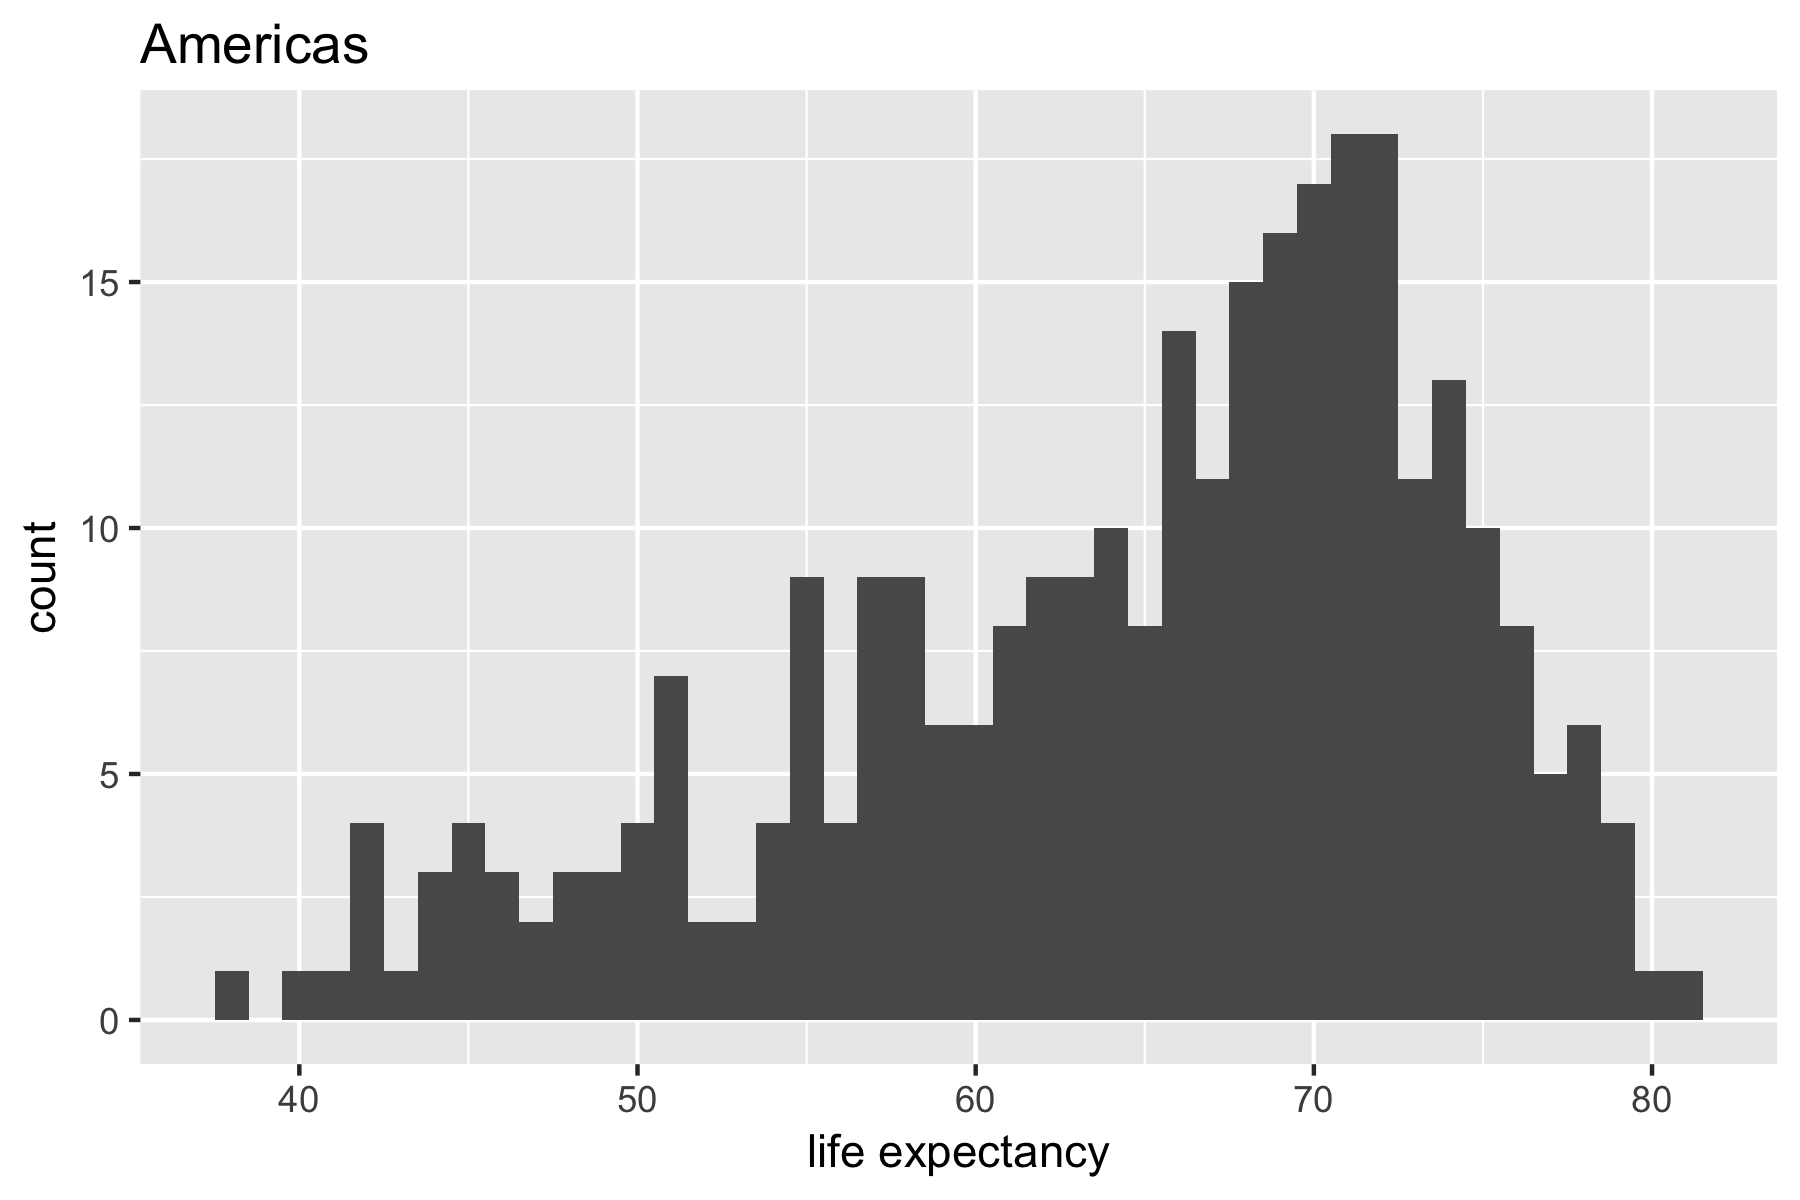
\includegraphics[width=0.75\textwidth]{figs/intro_cogs.png}
  % \subfigure[Caption of subfigure 2]{
  \subfigure{
    \small\ttfamily

% latex table generated in R 3.4.1 by xtable 1.8-2 package
% Wed Nov  1 20:57:16 2017
\begin{tabular}{llr}
  \toprule
 \textnormal{group} & \textnormal{cog} & \textnormal{value} \\ 
  \midrule
   \_x & min & 37.58 \\ 
    & max & 80.65 \\ 
    & mean & 64.66 \\ 
    & median & 67.05 \\ 
  \bigskip  & var & 87.33 \\ 
   \_density\_x & max\_density & 0.05 \\ 
    & max\_density\_location & 70.14 \\ 
    & unimodal\_p\_value & 0.99 \\ 
    & skew & -0.74 \\ 
    & kurt & 2.81 \\ 
   \bottomrule
\end{tabular}
  }
  % \subfigure[Caption of subfigure 3]{
  \subfigure{
    \small\ttfamily

% latex table generated in R 3.4.1 by xtable 1.8-2 package
% Wed Nov  1 20:57:16 2017
\begin{tabular}{llr}
  \toprule
 \textnormal{group} & \textnormal{cog} & \textnormal{value} \\ 
  \midrule
   \_hist\_x & count\_min & 0.00 \\ 
    & count\_max & 18.00 \\ 
    & count\_mean & 6.82 \\ 
    & count\_median & 6.00 \\ 
    & count\_var & 25.78 \\ 
  \bigskip  & chisq & 0.00 \\ 
   \_n & n & 300.00 \\ 
    & n\_na & 0.00 \\ 
    &  &  \\ 
    &  &  \\ 
   \bottomrule
\end{tabular}
  }
\caption[\autocogs~automatically produces four cognostic groups for a single layer (histogram) plot]{\autocogs~automatically produces four cognostic groups for a single layer (histogram) plot shown above. These cognostic groups are shown in the two tables describing the cognostic group, name, and value.  All eighteen cognostics may be used within a \trelliscopejs~HTML widget to aid in sorting and filtering plot panels.}
\end{figure}
\renewcommand{\arraystretch}{1} % Default value: 1





\section{\gqlr: An R server GraphQL implementation}

In 2012, Facebook began development of GraphQL, a backend agnostic data query language and runtime.  Data query API that allows data to be queried without requiring knowledge how the data is stored.  In doing so, GraphQL drastically reduces the number of server requests created by the browser by using a dynamic and nested query structure.
For instance, when inspecting the names of a person's friends of their friends, it would normally require $O(n^2)$ query commands to finally realize the full answer where $n$ is the number of friends for each person.  With GraphQL, the dynamic query structure allows for the full request to be sent to the server and a single, albeit, larger answer is returned.  The submitted query command is separated from the actual backend service, moving the implementation complexity to the data backend service rather than the query submission process.
Figure~\ref{figs:intro_graphql} displays the reduction in communication between a web browser client and the data server for both a naive REST implementation and a GraphQL implementation.  The naive REST implementation requires $O(n^2)$ communications with the data server, while GraphQL executes a single communication with a single return value.
By decoupling the data servers with web pages, the development cycles of both the web pages and data servers are improved.
However, there is no prior interface of GraphQL to R. Therefore, in the third part of this thesis, I develop the \gqlr~R package, which implements a full GraphQL server within R.  \gqlr~allows R users to supply their own functions to satisfy the data requirements of a submitted GraphQL query, thus enjoying the rapid iteration time of R and production iteration time of GraphQL.


\begin{figure}[H]
  \label{figs:intro_graphql}
  \centering
  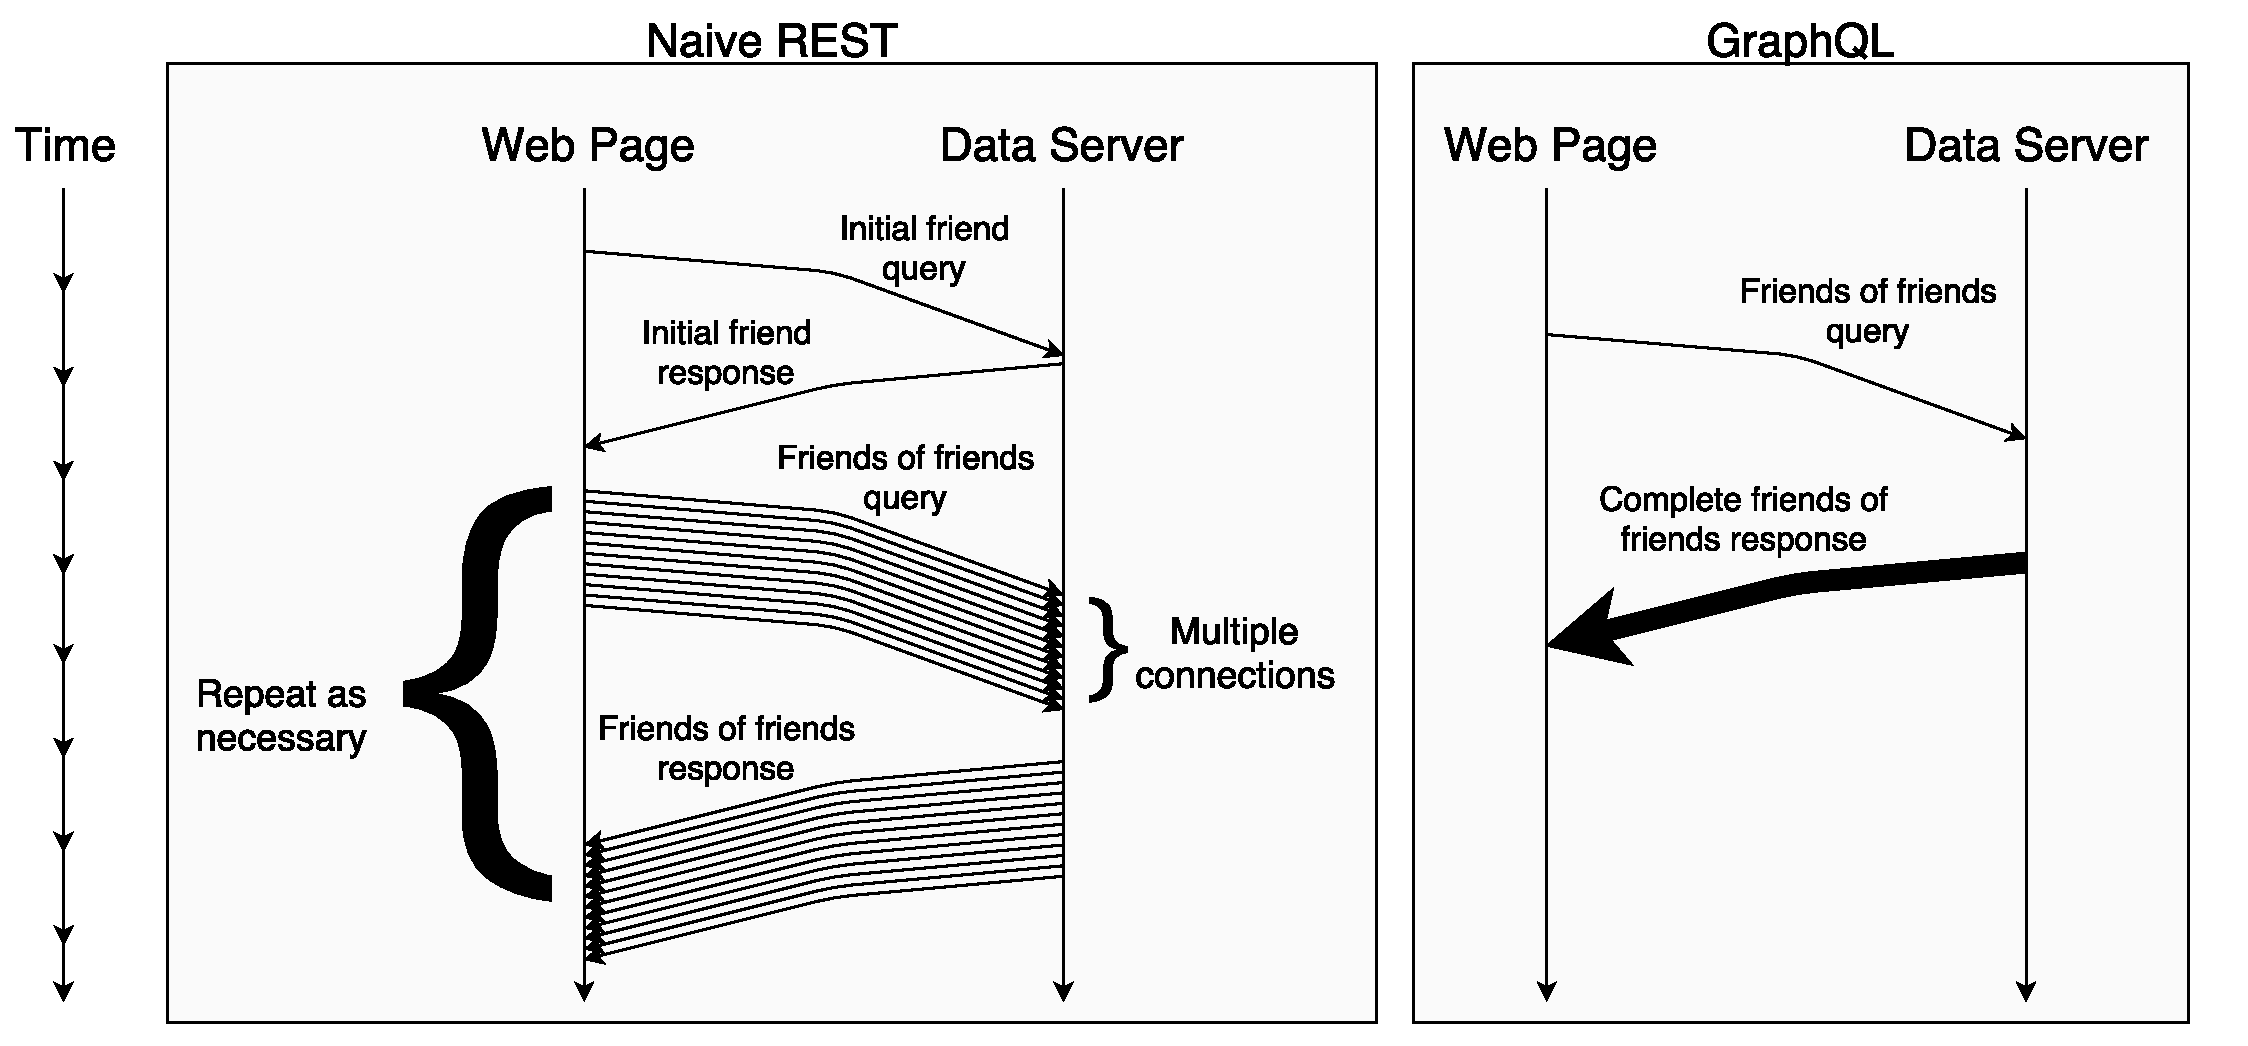
\includegraphics[width=\textwidth]{./figs/graphql_communication.pdf}
  \caption[``Friends of my friends'' GraphQL communication graph]{Time passes from top to bottom in this communication graph.  In ``friends of my friends'' example, the Naive REST implementation requires $O(n^2)$ queries (where $n$ is the number of friends for each person), while the GraphQL implementation solves the example query in a single communication to the data server.}
  % \vspace{10pt}
  \bigskip
\end{figure}








%
%
% \section{Related work}
%
% % verbose description of figure 1.1
% % <= 1 page in total
% % describe how i built on them and how i am different from them.
%
% % describe packages like ggplot2, rbokeh, plotly, lattice
%
%
%
\section{Thesis Organization}

The structure of this thesis is presented in Figure~\ref{fig:structure}.
The main contributions of this thesis include:
\begin{enumerate}[i)]
  \item \rinline{ggduo}, an R function in \GGally~that produces generalized plot matrices for two groups of variables (Chapter~\ref{chapter:ggduo}),
  \item \autocogs, an R package that automatically generates cognostics for a set of plots  (Chapter~\ref{chapter:autocogs}), and
  \item \gqlr, an R package which implements the GraphQL data query application protocol interface (Chapter~\ref{chapter:gqlr}).
\end{enumerate}

All components of this thesis are developed within the R environment and relate to the visualization and exploration of data.

Building on a grammar of graphics, \ggplot~is a layered plotting framework that \GGally~utilizes for visualizing data.  Each plot within the cell of a \rinline{ggmatrix} plot matrix is a fully defined \ggplot~plot object.  Using \rinline{ggmatrix} as a plot matrix foundation, two main functions apply different variable combinations to produce different plot matrices: \rinline{ggpairs}, a generalized pairs plot, and \rinline{ggduo}, a generalized plot matrix for two-grouped data.  \rinline{ggduo} is further extended by \rinline{ggnostic}, a generalized plot matrix for model diagnostics, and \rinline{ggts}, a generalized plot matrix for time series data.  In Chapter~\ref{chapter:ggduo}, I develop the generalized plot matrix for two-grouped data and its extensions.

In Chapter~\ref{chapter:autocogs}, I develop \autocogs, an R package that inspects a plot's data visualization layers to produce standard groups of cognostics.  Currently, \ggplot~plot objects are understood by \autocogs; in future work, \autocogs~will be able to understand how to automatically produce cognostics for plot objects produced by the popular R plotting libraries \pkg{plotly}, \pkg{lattice}, and \pkg{rbokeh}.  Once the cognostic groups are produced, they may be utilized within the interactive HTML widget \trelliscopejs~to sort and filter visualization panels.  The R package \pkg{htmlwidgets}~\cite{r_htmlwidgets} generates HTML widgets which facilitate interactive web visualizations in R.
\trelliscopejs~can display data visualization panels from many R packages, of which include \ggplot, \pkg{plotly}, \pkg{lattice}, and \pkg{rbokeh}.

In Chapter~\ref{chapter:gqlr}, I explore the GraphQL data query API and develop the R package \gqlr.  GraphQL was originally built to provide a consistent communication link between websites in the browser and data servers. The package  \gqlr~implements a GraphQL data server within the R environment. \gqlr~is built to handle GraphQL data queries and expose statistical routines provided by R and its packages. While \gqlr~was originally pursued to aid data extraction with \trelliscopejs, it will be integrated within \trelliscopejs~as development is continued.
% While not tied directly to any \pkg{htmlwidget},


\begin{figure}[H]
  \label{fig:structure}
  \centering
  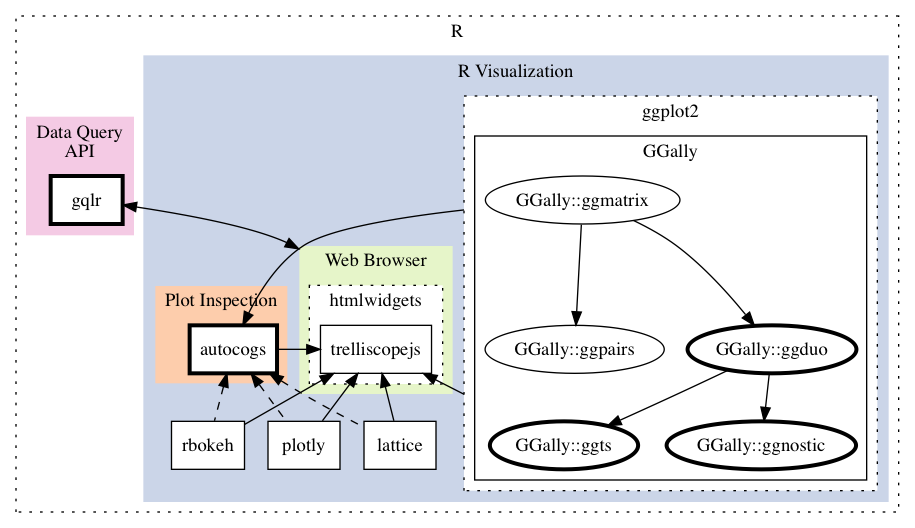
\includegraphics[width=\textwidth]{./dot/intro_hierarchy.png}
  \caption[Thesis Organization]{Thesis Organization.  Shaded regions represent different contexts within the R environment.  Black bordered square boxes represent R packages.   \GGally~is built upon \ggplot, and ellipses within \GGally~represent package functions.  Solid arrows represent functional dependencies or R package interactions.  Dashed arrows represent possible future interactions.  The bolded R packages and \GGally~functions correspond to different chapters within this thesis.  Summary descriptions of these packages are provided in Appendix~\ref{chapter:pkgs}.}
\end{figure}

% Put chapter \include commands here.


\chapter{GGDUO: GENERALIZED PAIRS PLOT FOR TWO-GROUPED DATA} \label{chapter:ggduo}











\section{\ggplot}

  % \ggplot~is different from the standard visualization graphics in that
  %
  %

  % \subsection{The Grammar of Graphics}

  % \emph{The Grammar of Graphics}~\cite{WilkinsonLeland2005TGoG} by Dr. Leland Wilkinson was originally released in 1999 and updated in 2005.  In his book, he ``presents a unique foundation for producing almost every quantitative graphic''~\cite{WilkinsonLeland2005TGoG}.  Dr. Wilkinson's graphical foundation helped give book is used at the core philosophy of \ggplot~with


% Grammar of graphics
%   By Leland Wilkinson in 1999 and 2005
%   ``This book was written for statisticians, computer scientists, geographers, research and applied scientists, and others interested in visualizing data. It presents a unique foundation for producing almost every quantitative graphic found in scientific journals, newspapers, statistical packages, and data visualization systems. This foundation was designed for a distributed computing environment (Internet, Intranet, client-server), with special attention given to conserving computer code and system resources.''





\subsection{\emph{Layered Grammar of Graphics}}

The R data visualization package \ggplot~is based on a \emph{Layered Grammar of Graphics}~\cite{layered_grammar}.  During consulting meetings with students and faculty in helping them produce statistical visualizations of their data, the authors of the package noticed that many clients had trouble producing plots quickly and have difficulties understanding how the plots were generated.  This motivated them to develop the \ggplot~package, which is based on the foundations of \emph{The Grammar of Graphics}~\cite{}.

\subsection{\ggplot~layers}

Most of the standard statistical graphical displays take the form of single-layered plots.  For example, a scatterplot consists of a point layer while a boxplot contains a boxplot layer.  There is no formal name for the data graphic where horizontally jittered points are displayed on top of a vertical boxplot.  Each layer is understood as a component to the plot, therefore the plot as a whole can be understood.  Wickham did state that while a layered grammar guides a well formed graphic~\cite{layered_grammar}, he analogizes ``good grammar is just the first step in creating a good sentence''~\cite{layered_grammar}.

Each plot consists of three components: the data, geom, and scales. Respectively, each of the component defines what is being displayed, how it is displayed and where it is being displayed.  By inferring from the supplied data source and geom defaults, many plots can be displayed without much coding.

\begin{knitrout}\small
\definecolor{shadecolor}{rgb}{0.969, 0.969, 0.969}\color{fgcolor}\begin{kframe}
\begin{alltt}
\hlstd{p} \hlkwb{<-} \hlkwd{ggplot}\hlstd{(tips,} \hlkwd{aes}\hlstd{(total_bill, tip))} \hlopt{+}
  \hlkwd{geom_point}\hlstd{()}
\hlstd{p}
\end{alltt}
\end{kframe}\begin{figure}[H]

{\centering \includegraphics[width=4in,height=3in]{figure/geom_point-1} 

}

\caption{Minimal coding for a scatterplot of \rinline{tips} data.}\label{fig:geom_point}
\end{figure}


\end{knitrout}

Typically, each layer of a plot uses the same data source to explore different aspects of the data set.  Multi-layered plots may use multiple data sources where it would not be appropriate to combine into a single data source.  Added data sources usually display contextual information (such as a map) or summary statistics (such as a mean or linear model).  Figure~\ref{fig:tip_lm} manually adds a linear model line on top of a scatterplot.

\begin{knitrout}\small
\definecolor{shadecolor}{rgb}{0.969, 0.969, 0.969}\color{fgcolor}\begin{kframe}
\begin{alltt}
\hlstd{tip_lm} \hlkwb{<-} \hlstd{broom}\hlopt{::}\hlkwd{tidy}\hlstd{(}\hlkwd{lm}\hlstd{(tip} \hlopt{~} \hlstd{total_bill,} \hlkwc{data} \hlstd{= tips))}\hlopt{$}\hlstd{estimate}
\hlstd{(tip_lm_dt} \hlkwb{<-} \hlkwd{data.frame}\hlstd{(}
  \hlkwc{intercept} \hlstd{= tip_lm[}\hlnum{1}\hlstd{],}
  \hlkwc{slope} \hlstd{= tip_lm[}\hlnum{2}\hlstd{]}
\hlstd{))}
\end{alltt}
\begin{verbatim}
##   intercept     slope
## 1 0.9202696 0.1050245
\end{verbatim}
\begin{alltt}
\hlstd{p} \hlopt{+}
  \hlkwd{geom_abline}\hlstd{(}
    \hlkwc{data} \hlstd{= tip_lm_dt,}
    \hlkwd{aes}\hlstd{(}\hlkwc{slope} \hlstd{= slope,} \hlkwc{intercept} \hlstd{= intercept)}
  \hlstd{)}
\end{alltt}
\end{kframe}\begin{figure}[H]

{\centering \includegraphics[width=4in,height=3in]{figure/tip_lm-1} 

}

\caption{Scatterplot with a linear model line added using a different data source.}\label{fig:tip_lm}
\end{figure}


\end{knitrout}



% What is a layered plot


% Each layer allows for default argument values to be used instead of being supplied in every layer.  With decent default values, every argument does not need to be supplied as is described in Grammar of Graphics.

\subsection{Plot creation}

All plot layers do not need to exist at the time of plot object inception.  Each layer of a \ggplot~plot may be added one by one to the original plot object at different times of the code execution.  The simplist of plot objects consists of a default data set and a default set of aesthetics.

\begin{knitrout}\small
\definecolor{shadecolor}{rgb}{0.969, 0.969, 0.969}\color{fgcolor}\begin{kframe}
\begin{alltt}
\hlstd{minimal_plot} \hlkwb{<-} \hlkwd{ggplot}\hlstd{(}\hlkwc{data} \hlstd{= tips,} \hlkwd{aes}\hlstd{(total_bill, tip))}
\hlcom{# perform extra calculations}
\hlnum{1} \hlopt{+} \hlnum{1}
\end{alltt}
\begin{verbatim}
## [1] 2
\end{verbatim}
\begin{alltt}
\hlcom{# plot display delayed until print time}
\hlstd{minimal_plot}
\end{alltt}
\end{kframe}\begin{figure}[H]

{\centering \includegraphics[width=4in,height=3in]{figure/minimal_gg-1} 

}

\caption{Empty \ggplot~plot with no layers displayed after extra calculations.}\label{fig:minimal_gg}
\end{figure}


\end{knitrout}

No layers are displayed as none have been provided.  However, the scales have been infered from the data aesthetics: $X$: \rinline{total_bill} and $Y$: \rinline{tip}.

\subsection{Comparison}

Building the plot up layer by layer and storing it as an R object until printed does not follow the existing patterns in standard R graphics.  In Figure~\ref{fig:graphics_plot}, the R core package \pkg{graphics}~\cite{r_project} displays information in a plot immediately upon function call.  There is no ability to delay the display of the plot after the initial plot function has been called when using the \pkg{graphics}~package.

\begin{knitrout}\small
\definecolor{shadecolor}{rgb}{0.969, 0.969, 0.969}\color{fgcolor}\begin{kframe}
\begin{alltt}
\hlstd{g} \hlkwb{<-} \hlstd{graphics}\hlopt{::}\hlkwd{plot}\hlstd{(tip} \hlopt{~} \hlstd{total_bill,} \hlkwc{data} \hlstd{= tips)}
\end{alltt}
\end{kframe}\begin{figure}[H]

{\centering \includegraphics[width=4in,height=3in]{figure/graphics_plot-1} 

}

\caption{Stock R scatterplot using the \pkg{graphics}~package is printed immediately.}\label{fig:graphics_plot}
\end{figure}

\begin{kframe}\begin{alltt}
\hlcom{# nothing is stored, as plot is already displayed}
\hlstd{g}
\end{alltt}
\begin{verbatim}
## NULL
\end{verbatim}
\end{kframe}
\end{knitrout}

\pkg{lattice}~graphics meets in between \ggplot~and \pkg{graphics}, as all layers must be supplied at plot creation, but the plot is not displayed until print time.  Two prior \ggplot~examples, Figure~\ref{fig:geom_point} and Figure~\ref{fig:minimal_gg}, both displayed the ability to delay the printing of the \ggplot~plot object.  \pkg{lattice}~graphics can also delay the display of the plot object as shown in Figure~\ref{fig:lattice_xyplot}.  At print time, both \pkg{lattice}~and \ggplot~convert their internal plot objects to be displayed using the \pkg{grid}~package.  The \pkg{grid}~package does not implement full statistical plots, but rather it implements a R plotting framework to be used by other packages like \ggplot~and \pkg{lattice}.

\begin{knitrout}\small
\definecolor{shadecolor}{rgb}{0.969, 0.969, 0.969}\color{fgcolor}\begin{kframe}
\begin{alltt}
\hlstd{l} \hlkwb{<-} \hlstd{lattice}\hlopt{::}\hlkwd{xyplot}\hlstd{(tip} \hlopt{~} \hlstd{total_bill,} \hlkwc{data} \hlstd{= tips)}
\hlcom{# display plot}
\hlstd{l}
\end{alltt}
\end{kframe}\begin{figure}[H]

{\centering \includegraphics[width=4in,height=3in]{figure/lattice_xyplot-1} 

}

\caption{\pkg{lattice}~scatterplot displaying using the \pkg{grid}~framework.}\label{fig:lattice_xyplot}
\end{figure}


\end{knitrout}

Finally, after executing the \pkg{graphics}~and \pkg{lattice}~examples, we can add a point layer to the minimal \ggplot~plot example in Figure~\ref{fig:minimal_point}.

\begin{knitrout}\small
\definecolor{shadecolor}{rgb}{0.969, 0.969, 0.969}\color{fgcolor}\begin{kframe}
\begin{alltt}
\hlcom{# layer added after plot inception}
\hlstd{minimal_points} \hlkwb{<-} \hlstd{minimal_plot} \hlopt{+} \hlkwd{geom_point}\hlstd{()}
\hlcom{# displays plot}
\hlstd{minimal_points}
\end{alltt}
\end{kframe}\begin{figure}[H]

{\centering \includegraphics[width=4in,height=3in]{figure/minimal_point-1} 

}

\caption{Adding a `point' layer to the base \ggplot~plot object created in an earlier code chunk.}\label{fig:minimal_point}
\end{figure}


\end{knitrout}

Modularization of the \ggplot~code allows for customization of each layer added to the plot.  This leads to a smaller, more consistent interface for each layer function.



\section{Facets}

% This is very important
%   ggplot2 does not create new columns of information
%     only performs minimal, common statistical transformations on existing columns such as binning and density
%   ggplot2 does not divide the data up in `cut' formats that do not exist in input data
%     only divides data (facets) according to pre-existing column combinations


Winston Chang, maintainer of \ggplot, explains facet'ing as ``[ploting] subsets of data into separate panels''~\cite{chang2013rgc}.  This is achieved using existing conditioning variables in the supplied data set. For each conditioning combination, a panel is produced. This technique commonly refered to as small multiples~\cite{small_multiples}.  The same style of plot is displayed, but each plot is constructed from an independent subset of the data.  Typically, only one or two conditioning variables are used, but any number of variables may be used when creating small multiples or faceting a \ggplot~plot.

Facets are useful when looking at the interaction of conditioning variables.  Once all existing combinations of the conditioning variables have been made, subsets of the data are displayed in each of the panels with the strip (panel label) of the panel displaying the conditioning variable information.  Missing combinations can either be dropped or display an empty panel.  \ggplot's wrapping facet will drop missing combinations by default, and \ggplot's faceted grid will display an empty panel for missing combinations.  In \ggplot, all variables are considered discrete when used as conditioning variables.


\subsection{Facet wrap}

There are two types of faceting in \ggplot: facet wrap and facet grid.  Facet wrap displays each panel starting from the top row to the bottom row and left to right within each row.  The number of rows and / or columns can be specified to ease the guessing work made by \ggplot.  If no facet row or column counts are supplied, \ggplot~uses \pkg{grDevices}~\cite{r_project} algorithm, \rinline{n2mfrow(n)}, to determine a sensible number of rows and columns.  Figure~\ref{fig:facets1} contains no faceting variables, while Figure~\ref{fig:facets2} and Figure~\ref{fig:facets3} condition on one and two variables respectively.


\begin{knitrout}\small
\definecolor{shadecolor}{rgb}{0.969, 0.969, 0.969}\color{fgcolor}\begin{kframe}
\begin{alltt}
\hlstd{p} \hlkwb{<-} \hlkwd{ggplot}\hlstd{(tips,} \hlkwd{aes}\hlstd{(total_bill, tip))} \hlopt{+} \hlkwd{geom_point}\hlstd{()}
\hlstd{p} \hlopt{+}
  \hlkwd{labs}\hlstd{(}\hlkwc{title} \hlstd{=} \hlstr{"No Facets"}\hlstd{)}
\end{alltt}
\end{kframe}\begin{figure}[H]

{\centering \includegraphics[width=4in,height=3in]{figure/facets1-1} 

}

\caption{$tip$ vs $total\_bill$ with facets or conditioning variables.}\label{fig:facets1}
\end{figure}


\end{knitrout}
\newpage
\begin{knitrout}\small
\definecolor{shadecolor}{rgb}{0.969, 0.969, 0.969}\color{fgcolor}\begin{kframe}
\begin{alltt}
\hlstd{p} \hlopt{+}
  \hlkwd{facet_wrap}\hlstd{(}\hlopt{~} \hlstd{day,} \hlkwc{labeller} \hlstd{= label_both)} \hlopt{+}
  \hlkwd{labs}\hlstd{(}\hlkwc{title} \hlstd{=} \hlstr{"Facet Wrap (~ day)"}\hlstd{)}
\end{alltt}
\end{kframe}\begin{figure}[H]

{\centering \includegraphics[width=4in,height=3in]{figure/facets2-1} 

}

\caption{$tip$ vs $total\_bill$ faceted by $day$. Each panel belongs to a given day in the data.}\label{fig:facets2}
\end{figure}


\end{knitrout}
\newpage
\begin{knitrout}\small
\definecolor{shadecolor}{rgb}{0.969, 0.969, 0.969}\color{fgcolor}\begin{kframe}
\begin{alltt}
\hlstd{p} \hlopt{+}
  \hlkwd{facet_wrap}\hlstd{(}\hlopt{~} \hlstd{day} \hlopt{+} \hlstd{time,} \hlkwc{labeller} \hlstd{= label_both)} \hlopt{+}
  \hlkwd{labs}\hlstd{(}\hlkwc{title} \hlstd{=} \hlstr{"Facet Wrap (~ day + time)"}\hlstd{)}
\end{alltt}
\end{kframe}\begin{figure}[H]

{\centering \includegraphics[width=4in,height=3in]{figure/facets3-1} 

}

\caption{$tip$ vs $total\_bill$ faceted by all existing $day$ and $time$ combinations.}\label{fig:facets3}
\end{figure}


\end{knitrout}

\subsection{Facet grid}

Facet grid forces a two dimensional, matrix-like layout when faceting a plot.  The layout involves two sets of conditioning variables: the X conditioning variables and the Y conditioning variables.  These two sets of conditioning variables pre-determine how many rows (Y) and columns (X) are presented.

\newpage
\begin{knitrout}\small
\definecolor{shadecolor}{rgb}{0.969, 0.969, 0.969}\color{fgcolor}\begin{kframe}
\begin{alltt}
\hlstd{p} \hlopt{+}
  \hlkwd{facet_grid}\hlstd{(time} \hlopt{~} \hlstd{day,} \hlkwc{labeller} \hlstd{= label_both)} \hlopt{+}
  \hlkwd{labs}\hlstd{(}\hlkwc{title} \hlstd{=} \hlstr{"Facet Grid (time ~ day)"}\hlstd{)}
\end{alltt}
\end{kframe}\begin{figure}[H]

{\centering \includegraphics[width=4in,height=3in]{figure/facet_grid_example-1} 

}

\caption{$tip$ vs $total\_bill$ faceted in a grid pattern with $time$ representing each row and $day$ representing each column.}\label{fig:facet_grid_example}
\end{figure}


\end{knitrout}

Figure~\ref{fig:facet_grid_example} displays $time$ on the rows ($Y$) and $day$ on the columns ($X$).  The \rinline{facet_grid} formula follows the R \rinline{stats::lm} linear model formula of \rinline{y ~ x}.  Multiple variables can be used in either the $X$ position or the $Y$ position.  This allows the user to display a column combination set against another column combination set.  Using multiple conditioning variables within facet grid in Figure~\ref{fig:facet_grid_multi}, both Male and Female smokers during Sunday Dinner tip value does not follow a positive linear trend as the total bill increases.

\newpage
% do not change size
\begin{knitrout}\small
\definecolor{shadecolor}{rgb}{0.969, 0.969, 0.969}\color{fgcolor}\begin{kframe}
\begin{alltt}
\hlstd{p} \hlopt{+}
  \hlkwd{geom_smooth}\hlstd{(}\hlkwc{method} \hlstd{= lm,} \hlkwc{se} \hlstd{=} \hlnum{FALSE}\hlstd{)} \hlopt{+}
  \hlkwd{facet_grid}\hlstd{(sex} \hlopt{+} \hlstd{smoker} \hlopt{~} \hlstd{time} \hlopt{+} \hlstd{day,} \hlkwc{labeller} \hlstd{= label_both)}
\end{alltt}
\end{kframe}\begin{figure}[H]

{\centering \includegraphics[width=5.5in,height=4.125in]{figure/facet_grid_multi-1} 

}

\caption{$tip$ vs $total\_bill$ faceted in a grid pattern with $sex$ and $smoker$ combinations representing each row and $time$ and $day$ combinations representing each column.}\label{fig:facet_grid_multi}
\end{figure}


\end{knitrout}



\section{Plot matrix}

\rinline{ggduo} is continuation of prior work in the \GGally~R package.  In this section, I will cover how a pairs plot is different than a small multiple, background on the scatterplot matrix and generalized pairs plot matrix, and the \rinline{ggmatrix} object that generalized the plot matrix used in \rinline{ggduo}.


\subsection{Pairs plot}

  As mentioned earlier in the chapter, \ggplot~is designed to allow plots to be built layer by layer and not rendered until a final print command is executed.  \ggplot~plot objects has some implementation rules it follows when faceting a plot:

  \begin{enumerate}
    \item Each faceted panel must share the same original $X$ and $Y$ columns.
    \item Each faceted panel's data must be independent of all other panels in the same plot.
    \item Each plot must be created with the same layers.
  \end{enumerate}

  Following these rules allows for the implementation of small multiples.  Small multiples are repetitions of plots with identical layers, but each plot is comprised of different data.  Small multiples were popularized by \emph{Edward Tufte} in his 1983 paper Visual Display of Quantitative Information~\cite{tufte_display_info}.  The \rinline{facet_wrap} and \rinline{facet_grid} functions will produce a multi-panel output in the form of small multiples.

  A pairs plot, originally referred to as a ``draftsman's plot''~\cite{GraphicalMethods},  violates all three principles of a small multiple:

  \begin{enumerate}
    \item Each panel is comprised of a different $X$ and $Y$ combination.
    \item Each panel shares the same underlying data.
    \item Each panel may be created with different layers that better suited for the data types.
  \end{enumerate}


  The original scatterplot matrix was only displayed using a scatterplot for each sub panel.  \emph{The Generalized Pairs Plot} by Emerson et. al., suggested that a pairs plot should not be restricted to just continuous scatterplots.  A pairs plot should be generalized to allow for discrete data to be displayed as well as continuous data.  A scatterplot matrix is not appropriate for discrete data.  In a discrete data versus discrete data plot, all of the data points would be overplotted onto the unique discrete combinations.  This overplotting renders the discrete only pairs plot combinations uninterpretable.  The bottom right quadrant of the pairs plot in Figure~\ref{fig:original_pairs} display eight unique points between $smoker$ and $day$, but do not convey that they really contain 244 points.

\begin{knitrout}\small
\definecolor{shadecolor}{rgb}{0.969, 0.969, 0.969}\color{fgcolor}\begin{kframe}
\begin{alltt}
\hlstd{graphics}\hlopt{::}\hlkwd{pairs}\hlstd{(tips[}\hlkwd{c}\hlstd{(}\hlstr{"total_bill"}\hlstd{,} \hlstr{"tip"}\hlstd{,} \hlstr{"smoker"}\hlstd{,} \hlstr{"day"}\hlstd{)])}
\end{alltt}
\end{kframe}\begin{figure}[H]

{\centering \includegraphics[width=5.5in,height=4.125in]{figure/original_pairs-1} 

}

\caption{Stock R graphics scatterplot matrix displaying the \rinline{tips} data set.}\label{fig:original_pairs}
\end{figure}


\end{knitrout}

  Emerson et.al. discussed using a generalized pairs plot to handle the mix of variable types by providing different plotting layers for different data types.  The generalized pairs plot displays the same collection of data using different axes but allows for a mix of plotting methods with both continuous and discrete plot axes.  This addresses the issue of overplotting in discrete columns when displaying data in a scatterplot matrix.  Figure~\ref{fig:gpairs_intro} and Figure~\ref{fig:ggpairs_intro} are two plotting methods to handle the discrete data overplotting issue.  The \pkg{gpairs}~\cite{r_gpairs} R package is printed using \pkg{lattice}~graphics (Figure~\ref{fig:gpairs_intro}), while the \GGally~R package prints using \ggplot~graphics (Figure~\ref{fig:ggpairs_intro}).

\begin{knitrout}\small
\definecolor{shadecolor}{rgb}{0.969, 0.969, 0.969}\color{fgcolor}\begin{kframe}
\begin{alltt}
\hlstd{gpairs}\hlopt{::}\hlkwd{gpairs}\hlstd{(tips[,} \hlkwd{c}\hlstd{(}\hlstr{"total_bill"}\hlstd{,} \hlstr{"tip"}\hlstd{,} \hlstr{"smoker"}\hlstd{,} \hlstr{"day"}\hlstd{)])}
\end{alltt}
\end{kframe}\begin{figure}[H]

{\centering \includegraphics[width=5.5in,height=4.125in]{figure/gpairs_intro-1} 

}

\caption{\rinline{gpairs}~plot matrix from the \pkg{gpairs}~R package displaying the \rinline{tips} data set.}\label{fig:gpairs_intro}
\end{figure}


\end{knitrout}

\newpage
\begin{knitrout}\small
\definecolor{shadecolor}{rgb}{0.969, 0.969, 0.969}\color{fgcolor}\begin{kframe}
\begin{alltt}
\hlstd{pm} \hlkwb{<-} \hlkwd{ggpairs}\hlstd{(tips,} \hlkwd{c}\hlstd{(}\hlstr{"total_bill"}\hlstd{,} \hlstr{"tip"}\hlstd{,} \hlstr{"smoker"}\hlstd{,} \hlstr{"day"}\hlstd{))}
\hlstd{pm}
\end{alltt}
\end{kframe}\begin{figure}[H]

{\centering \includegraphics[width=5.5in,height=4.125in]{figure/ggpairs_intro-1} 

}

\caption{\rinline{ggpairs}~plot matrix from the \GGally~R package displaying the \rinline{tips} data set.}\label{fig:ggpairs_intro}
\end{figure}


\end{knitrout}

\rinline{gpairs::gpairs} was originally built to handle the generalization of the pairs plot to include discrete data.  Unfortunately, this is written using \pkg{lattice}~graphics and does not utilize the \ggplot~framework.  \rinline{GGally::ggpairs} was originally written as an independent port of of \rinline{gpairs} to the \ggplot~framework but with portability and modularization kept in mind.

\GGally's \rinline{ggpairs} addressed the portability and modularization by
\begin{enumerate}
  \item making each sub plot an independently functioning \ggplot~plot.  Figure~\ref{fig:add_custom_plot} displays how a sub plot may be retrieved.
  \item allowing each sub plot to be replaced after the initial plot matrix is created.  Figure~\ref{fig:add_custom_plot2} creates a new plot that is placed inside the matrix in Figure~\ref{fig:add_custom_plot3}.
  \item and not displaying the plot matrix until the \rinline{print} command is executed.  Similar to earlier \ggplot~examples, the displaying of a \GGally~plot matrix is delayed until print time as in Figure~\ref{fig:add_custom_plot3}.
\end{enumerate}

\begin{knitrout}\small
\definecolor{shadecolor}{rgb}{0.969, 0.969, 0.969}\color{fgcolor}\begin{kframe}
\begin{alltt}
\hlcom{# retrieve the second row, first column sub plot}
\hlcom{#  of the tips plot matrix}
\hlstd{pm[}\hlnum{2}\hlstd{,}\hlnum{1}\hlstd{]}
\end{alltt}
\end{kframe}\begin{figure}[H]

{\centering \includegraphics[width=4in,height=3in]{figure/add_custom_plot-1} 

}

\caption{Full \ggplot~plot object from the second row and first column of a \rinline{ggmatrix} plot matrix.}\label{fig:add_custom_plot}
\end{figure}


\end{knitrout}
\newpage
\begin{knitrout}\small
\definecolor{shadecolor}{rgb}{0.969, 0.969, 0.969}\color{fgcolor}\begin{kframe}
\begin{alltt}
\hlstd{replacement_plot} \hlkwb{<-} \hlkwd{ggally_text}\hlstd{(}
  \hlstr{"Replacement\textbackslash{}nPlot"}\hlstd{,}
  \hlkwd{aes}\hlstd{(}\hlkwc{color} \hlstd{=} \hlstr{"red"}\hlstd{),}
  \hlkwc{size} \hlstd{=} \hlnum{6}
\hlstd{)}
\hlstd{replacement_plot}
\end{alltt}
\end{kframe}\begin{figure}[H]

{\centering \includegraphics[width=4in,height=3in]{figure/add_custom_plot2-1} 

}

\caption{Replacement plot displaying ``Replacement Plot'' in red.}\label{fig:add_custom_plot2}
\end{figure}


\end{knitrout}
\newpage
\begin{knitrout}\small
\definecolor{shadecolor}{rgb}{0.969, 0.969, 0.969}\color{fgcolor}\begin{kframe}
\begin{alltt}
\hlcom{# insert the new plot into the second row, first column}
\hlcom{#  of the tips plot matrix}
\hlstd{pm[}\hlnum{2}\hlstd{,}\hlnum{1}\hlstd{]} \hlkwb{<-} \hlstd{replacement_plot}
\hlcom{# display the updated plot matrix}
\hlstd{pm}
\end{alltt}
\end{kframe}\begin{figure}[H]

{\centering \includegraphics[width=5.5in,height=4.125in]{figure/add_custom_plot3-1} 

}

\caption{The replacement plot is placed in the second row and first column.  The updated plot matrix is displayed.}\label{fig:add_custom_plot3}
\end{figure}


\end{knitrout}


\subsection{\rinline{ggmatrix}}

The \rinline{ggmatrix} object is used to handle two main situations: handle mixed plot scales and contain the necessary information for displaying a plot matrix.

\subsubsection{Plot scales}

\ggplot~prevents discrete scales from being mixed with continuous scales.  Two different scales for the same axis is not possible in a multi panel \ggplot~plot as \ggplot~is built on the small multiple princple of displaying similar scales in every faceted panel.  Only one scale type is used per ggmatrix panel.  This keeps the original `per panel' logic intact.

Produce two related mixed-axes plots in the same graphic could only be achieved using the \pkg{gridExtra}~\cite{gridExtra} or \pkg{grid}~\cite{r_project} R packages before \rinline{ggmatrix}.  Both of these existing methods behaved like a side by side, fully printed plots, rather than a native plot matrix.

\begin{knitrout}\small
\definecolor{shadecolor}{rgb}{0.969, 0.969, 0.969}\color{fgcolor}\begin{kframe}
\begin{alltt}
\hlstd{p1} \hlkwb{<-} \hlstd{pm[}\hlnum{1}\hlstd{,}\hlnum{4}\hlstd{]}
\hlstd{p2} \hlkwb{<-} \hlstd{pm[}\hlnum{2}\hlstd{,}\hlnum{4}\hlstd{]}
\hlstd{gridExtra}\hlopt{::}\hlkwd{grid.arrange}\hlstd{(p1, p2,} \hlkwc{ncol} \hlstd{=} \hlnum{1}\hlstd{)}
\end{alltt}
\end{kframe}\begin{figure}[H]

{\centering \includegraphics[width=4in,height=3in]{figure/grid_extra-1} 

}

\caption{Two fully displayed \ggplot~plot objects arranged using \pkg{gridExtra}. Duplicate axes and labels are present.  The $X$ axis does not align as the plots are treated independently.  It appears as two independent plots in one display.}\label{fig:grid_extra}
\end{figure}


\end{knitrout}

\rinline{ggmatrix} allows for arbitrary scales per panel. When used properly, independently produced sub plots deliver common axes within each row and column.  This displays a cohesive and interpretable plot matrix structure.


\subsubsection{Display information}

The necessary information includes the number of rows and columns, label information, \ggplot~display theme information,  how plot strips should be displayed, default plot data, and individual plot information.

\begin{knitrout}\scriptsize
\definecolor{shadecolor}{rgb}{0.969, 0.969, 0.969}\color{fgcolor}\begin{kframe}
\begin{alltt}
\hlkwd{str}\hlstd{(pm)}
\end{alltt}
\begin{verbatim}
## 
## Custom str.ggmatrix output: 
## To view original object use 'str(pm, raw = TRUE)'
## 
## List of 19
##  $ data               :'data.frame':	244 obs. of  7 variables:
##   ..$ total_bill: num [1:244] 17 10.3 21 23.7 24.6 ...
##   ..$ tip       : num [1:244] 1.01 1.66 3.5 3.31 3.61 4.71 2 3.12 1.96 3.23 ...
##   ..$ sex       : Factor w/ 2 levels "Female","Male": 1 2 2 2 1 2 2 2 2 2 ...
##   ..$ smoker    : Factor w/ 2 levels "No","Yes": 1 1 1 1 1 1 1 1 1 1 ...
##   ..$ day       : Factor w/ 4 levels "Thur","Fri","Sat",..: 4 4 4 4 4 4 4 4 4 4 ...
##   ..$ time      : Factor w/ 2 levels "Lunch","Dinner": 2 2 2 2 2 2 2 2 2 2 ...
##   ..$ size      : int [1:244] 2 3 3 2 4 4 2 4 2 2 ...
##  $ plots              :List of 16
##   ..$ : chr "PM; aes: c(x = total_bill); fn: {wrap: 'ggally_densityDiag'}; gg: FALSE"
##   ..$ : chr "PM; aes: c(x = tip, y = total_bill); fn: {wrap: 'ggally_cor'}; gg: FALSE"
##   ..$ : chr "PM; aes: c(x = smoker, y = total_bill); fn: {wrap: 'ggally_box_no_facet'}; gg: FALSE"
##   ..$ : chr "PM; aes: c(x = day, y = total_bill); fn: {wrap: 'ggally_box_no_facet'}; gg: FALSE"
##   ..$ : chr "PM; ggplot2 object; mapping: c()"
##   ..$ : chr "PM; aes: c(x = tip); fn: {wrap: 'ggally_densityDiag'}; gg: FALSE"
##   ..$ : chr "PM; aes: c(x = smoker, y = tip); fn: {wrap: 'ggally_box_no_facet'}; gg: FALSE"
##   ..$ : chr "PM; aes: c(x = day, y = tip); fn: {wrap: 'ggally_box_no_facet'}; gg: FALSE"
##   ..$ : chr "PM; aes: c(x = total_bill, y = smoker); fn: {wrap: 'ggally_facethist'}; gg: FALSE"
##   ..$ : chr "PM; aes: c(x = tip, y = smoker); fn: {wrap: 'ggally_facethist'}; gg: FALSE"
##   ..$ : chr "PM; aes: c(x = smoker); fn: {wrap: 'ggally_barDiag'}; gg: FALSE"
##   ..$ : chr "PM; aes: c(x = day, y = smoker); fn: {wrap: 'ggally_facetbar'}; gg: FALSE"
##   ..$ : chr "PM; aes: c(x = total_bill, y = day); fn: {wrap: 'ggally_facethist'}; gg: FALSE"
##   ..$ : chr "PM; aes: c(x = tip, y = day); fn: {wrap: 'ggally_facethist'}; gg: FALSE"
##   ..$ : chr "PM; aes: c(x = smoker, y = day); fn: {wrap: 'ggally_facetbar'}; gg: FALSE"
##   ..$ : chr "PM; aes: c(x = day); fn: {wrap: 'ggally_barDiag'}; gg: FALSE"
##  $ title              : NULL
##  $ xlab               : NULL
##  $ ylab               : NULL
##  $ showStrips         : NULL
##  $ xAxisLabels        : chr [1:4] "total_bill" "tip" "smoker" "day"
##  $ yAxisLabels        : chr [1:4] "total_bill" "tip" "smoker" "day"
##  $ showXAxisPlotLabels: logi TRUE
##  $ showYAxisPlotLabels: logi TRUE
##  $ labeller           : chr "label_value"
##  $ switch             : NULL
##  $ xProportions       : NULL
##  $ yProportions       : NULL
##  $ legend             : NULL
##  $ gg                 : NULL
##  $ nrow               : int 4
##  $ ncol               : int 4
##  $ byrow              : logi TRUE
##  - attr(*, "_class")= chr [1:2] "gg" "ggmatrix"
\end{verbatim}
\end{kframe}
\end{knitrout}

For memory optimization, each plot is stored as a function that will produce the \ggplot~plot at print time.  To do so, the data set provided at a \rinline{ggmatrix} inception sets a default data set to be used at print time.  If a new sub plot is stored after inception, the fully defined \ggplot~object is stored directly.

Similar to \ggplot's function \rinline{ggplot_gtable}, \rinline{ggmatrix_gtable} produces display only information that the \pkg{grid}~graphics framework uses to display the plot. To retrieve all necessary display information, \rinline{ggmatrix_gtable} executes \rinline{ggplot_gtable} for each sub plot individually, then extracts the required plotting display information (plotting area and possibly the panel strips) from each sub plot.  These sub plot panels are then placed inside the final plot matrix.

The resulting plot matrix is displayed with the exact same styling as \ggplot's \rinline{facet_grid}. This returns all the display theme styling and display constraints back onto \ggplot.  By displaying the \rinline{ggmatrix} as a \rinline{facet_grid} in \ggplot, titles, legends, and other common plot artifacts are able to be natively displayed.   Figure~\ref{fig:ggpairs_legend} displays a legend on the right side of the plot matrix using the legend from the sub plot at position $(3,1)$.  Figure~\ref{fig:ggpairs_legend_bottom} uses the \ggplot~theme functionality to move the legend to beneath the plot matrix panels.

\newpage
\begin{knitrout}\small
\definecolor{shadecolor}{rgb}{0.969, 0.969, 0.969}\color{fgcolor}\begin{kframe}
\begin{alltt}
\hlcom{# color the plots according to smoker}
\hlcom{# display legend from the 3rd row, 1st column plot}
\hlstd{pm} \hlkwb{<-} \hlkwd{ggpairs}\hlstd{(}
  \hlstd{tips,} \hlkwd{c}\hlstd{(}\hlstr{"total_bill"}\hlstd{,} \hlstr{"tip"}\hlstd{,} \hlstr{"smoker"}\hlstd{,} \hlstr{"day"}\hlstd{),}
  \hlkwc{mapping} \hlstd{=} \hlkwd{aes}\hlstd{(}\hlkwc{color} \hlstd{= smoker),}
  \hlkwc{legend} \hlstd{=} \hlkwd{c}\hlstd{(}\hlnum{3}\hlstd{,}\hlnum{1}\hlstd{)}
\hlstd{)}
\hlstd{pm}
\end{alltt}
\end{kframe}\begin{figure}[H]

{\centering \includegraphics[width=5.5in,height=4.125in]{figure/ggpairs_legend-1} 

}

\caption{\rinline{ggmatrix}~displaying a color legend on the right (default) side of the plot matrix.}\label{fig:ggpairs_legend}
\end{figure}


\end{knitrout}
\newpage
\begin{knitrout}\small
\definecolor{shadecolor}{rgb}{0.969, 0.969, 0.969}\color{fgcolor}\begin{kframe}
\begin{alltt}
\hlcom{# display legend on bottom using ggplot2 theme}
\hlstd{pm} \hlopt{+} \hlstd{ggplot2}\hlopt{::}\hlkwd{theme}\hlstd{(}\hlkwc{legend.position} \hlstd{=} \hlstr{"bottom"}\hlstd{)}
\end{alltt}
\end{kframe}\begin{figure}[H]

{\centering \includegraphics[width=5.5in,height=4.125in]{figure/ggpairs_legend_bottom-1} 

}

\caption{\rinline{ggmatrix}~moving the legend to the bottom using \ggplot's \rinline{theme} function.}\label{fig:ggpairs_legend_bottom}
\end{figure}


\end{knitrout}


\section{\rinline{ggduo}: Plot matrix for two-grouped data}

A pairs plot is defined as displaying every column of the data against every other column in the data.  This is effective in full data exploration.  If a data set has columns $A$, $B$, and $C$, $3^2 = 9$ combinations produced in a corresponding pairs plot: $A:A$, $A:B$, $A:C$, $B:A$, $B:B$, etc.. A pairs plot matrix can be generalized one step further by pairing two column groups against each other.

For the example just described, column set $\left\{ A, B, C\right\}$ is paired against the column set $\left\{ A, B, C\right\}$.  As expected, this produces a pairs plot.  However, this generalization allows us to produce a plot matrix of the combinations of $\left\{ A, B, C\right\}$ and $\left\{ D, E\right\}$, or any combination of two column sets.  Using the same underlying \rinline{ggmatrix} functionality, \rinline{ggduo} produces plot combinations of two-grouped data.

As a quick example, let us look at the Australian students' fifth grade $Math$, $Reading$, and $Science$ scores against their $gender$ and how many hours of $homework$ each student completed each week in Figure~\ref{fig:ggmatrix_scores}.

\begin{knitrout}\small
\definecolor{shadecolor}{rgb}{0.969, 0.969, 0.969}\color{fgcolor}\begin{kframe}
\begin{alltt}
\hlkwd{ggduo}\hlstd{(}
  \hlstd{australia_PISA2012,}
  \hlkwd{c}\hlstd{(}\hlstr{"gender"}\hlstd{,} \hlstr{"homework"}\hlstd{),}
  \hlkwd{c}\hlstd{(}\hlstr{"PV5MATH"}\hlstd{,} \hlstr{"PV5READ"}\hlstd{,} \hlstr{"PV5SCIE"}\hlstd{)}
\hlstd{)}
\end{alltt}
\end{kframe}\begin{figure}[H]

{\centering \includegraphics[width=4in,height=3in]{figure/ggmatrix_scores-1} 

}

\caption{$5^{th}$ grade Australian student scholasitc scores vs their $sex$ and hours of weekly homework.}\label{fig:ggmatrix_scores}
\end{figure}


\end{knitrout}

Comparing these two groups if we are interested in knowing if there is any difference in any score output given a child's sex and homework time.  A \rinline{ggpairs} plot would create within and identity combinations as well as the between combinations of the \rinline{ggduo} plot, which is undesired in this situation.



\subsection{Column types}

\rinline{ggduo} inspects and displays the data columns according to their variable type: continuous or discrete. There are three plot type groups that can be made from these two options:
\begin{itemize}
  \item continuous vs. continuous. A scatterplot is a continuous vs. continuous plot.
  \item continuous vs. discrete.  A box plot or grouped box plots is a continuous vs. discrete plot.
  \item and discrete vs. discrete. A ratio plot, or a plot that can display the \rinline{tips}'s $smoker$ vs. $day$ (eight combinations of 244 records) is a discrete vs. discrete plot.
\end{itemize}


\rinline{ggduo}'s default plotting behavior for continuous vs. continuous, or `continuous plot', is to produce a scatterplot with a loess smooth curve displayed on top of the points.
The default plotting behavior for discrete vs. discrete, or `discrete plot', is to summarize the data and display it as a ratio plot.  A ratio plot displays rectangles whose size is proportional to the counts of the value combination in both the $X$ and $Y$ direction.


The third group, continuous vs. discrete, is refered to as a `combination plot'. \rinline{ggduo} makes a distinction between the two possible combination plots: continuous vs. discrete (vertical combination plot) and discrete vs. continuous (horizontal combination plot). By default, \rinline{ggduo} displays grouped histograms for a horizontal combination plot and grouped box plots for a vertical combination plot as in Figure~\ref{fig:ggduo_types}.
\rinline{ggpairs} is able to handle the combination plot differently for the upper and lower triangle using the the \rinline{upper} and \rinline{lower} arguments as in Figure~\ref{fig:ggpairs_types}.  Unlike \rinline{ggpairs}, a distiction between a horizontal and vertical combination plot is made as there are no upper and lower triangle plot matrix sections in a \rinline{ggduo} plot as in Figure~\ref{fig:ggduo_types2}.

\newpage
\begin{knitrout}\small
\definecolor{shadecolor}{rgb}{0.969, 0.969, 0.969}\color{fgcolor}\begin{kframe}
\begin{alltt}
\hlkwd{ggpairs}\hlstd{(}
  \hlstd{tips,}
  \hlkwd{c}\hlstd{(}\hlstr{"total_bill"}\hlstd{,} \hlstr{"smoker"}\hlstd{,} \hlstr{"day"}\hlstd{,} \hlstr{"tip"}\hlstd{),}
  \hlkwc{upper} \hlstd{=} \hlkwd{list}\hlstd{(}\hlkwc{combo} \hlstd{=} \hlstr{"denstrip"}\hlstd{),}
  \hlkwc{lower} \hlstd{=} \hlkwd{list}\hlstd{(}\hlkwc{combo} \hlstd{=} \hlstr{"facetdensity"}\hlstd{)}
\hlstd{)}
\end{alltt}
\end{kframe}\begin{figure}[H]

{\centering \includegraphics[width=5.5in,height=4.125in]{figure/ggpairs_types-1} 

}

\caption{Altering the \rinline{ggpairs} upper and lower \rinline{combo} plot types.}\label{fig:ggpairs_types}
\end{figure}


\end{knitrout}

\newpage
\begin{knitrout}\small
\definecolor{shadecolor}{rgb}{0.969, 0.969, 0.969}\color{fgcolor}\begin{kframe}
\begin{alltt}
\hlkwd{ggduo}\hlstd{(}
  \hlstd{tips,}
  \hlkwd{c}\hlstd{(}\hlstr{"total_bill"}\hlstd{,} \hlstr{"smoker"}\hlstd{,} \hlstr{"day"}\hlstd{),}
  \hlkwd{c}\hlstd{(}\hlstr{"tip"}\hlstd{,} \hlstr{"time"}\hlstd{)}
\hlstd{)}
\end{alltt}
\end{kframe}\begin{figure}[H]

{\centering \includegraphics[width=5in,height=3in]{figure/ggduo_types-1} 

}

\caption{two-grouped plot matrix using \rinline{ggduo} with no upper or lower triangle areas.}\label{fig:ggduo_types}
\end{figure}


\end{knitrout}

\newpage
\begin{knitrout}\small
\definecolor{shadecolor}{rgb}{0.969, 0.969, 0.969}\color{fgcolor}\begin{kframe}
\begin{alltt}
\hlkwd{ggduo}\hlstd{(}
  \hlstd{tips,}
  \hlkwd{c}\hlstd{(}\hlstr{"total_bill"}\hlstd{,} \hlstr{"smoker"}\hlstd{,} \hlstr{"day"}\hlstd{),}
  \hlkwd{c}\hlstd{(}\hlstr{"tip"}\hlstd{,} \hlstr{"time"}\hlstd{),}
  \hlkwc{types} \hlstd{=} \hlkwd{list}\hlstd{(}
    \hlkwc{comboVertical} \hlstd{=} \hlstr{"denstrip"}\hlstd{,}
    \hlkwc{comboHorizontal} \hlstd{=} \hlstr{"facetdensity"}
  \hlstd{)}
\hlstd{)}
\end{alltt}
\end{kframe}\begin{figure}[H]

{\centering \includegraphics[width=5in,height=3in]{figure/ggduo_types2-1} 

}

\caption{Updating the combination types in a \rinline{ggduo} plot matrix.}\label{fig:ggduo_types2}
\end{figure}


\end{knitrout}


\subsection{User defined functions}

There are many plotting functions are provided by the \GGally~package, however they are not all encompassing.  The user may supply their own plotting functions for each panel type.  This allows for complete customization of every panel. For example, a violin plot is a combination style plot that is not included by default.  A user may create their own function that uses the function call API of \rinline{function(data, mapping, ...) { ... }}.  A sample custom function example is provided below in Figure~\ref{fig:user_defined}.

\begin{knitrout}\small
\definecolor{shadecolor}{rgb}{0.969, 0.969, 0.969}\color{fgcolor}\begin{kframe}
\begin{alltt}
\hlstd{my_violin} \hlkwb{<-} \hlkwa{function}\hlstd{(}\hlkwc{data}\hlstd{,} \hlkwc{mapping}\hlstd{,} \hlkwc{...}\hlstd{) \{}
  \hlkwd{ggplot}\hlstd{(}\hlkwc{data} \hlstd{= data,} \hlkwc{mapping} \hlstd{= mapping)} \hlopt{+}
    \hlkwd{geom_violin}\hlstd{(...)}
\hlstd{\}}
\hlkwd{ggduo}\hlstd{(}
  \hlstd{tips,}
  \hlkwd{c}\hlstd{(}\hlstr{"total_bill"}\hlstd{,} \hlstr{"smoker"}\hlstd{,} \hlstr{"day"}\hlstd{),}
  \hlkwd{c}\hlstd{(}\hlstr{"tip"}\hlstd{,} \hlstr{"time"}\hlstd{),}
  \hlkwc{types} \hlstd{=} \hlkwd{list}\hlstd{(}
    \hlkwc{comboVertical} \hlstd{= my_violin}
  \hlstd{)}
\hlstd{)}
\end{alltt}
\end{kframe}\begin{figure}[H]

{\centering \includegraphics[width=5in,height=3in]{figure/user_defined-1} 

}

\caption{Use a custom function to display a plot within a \rinline{ggduo} plot matrix.}\label{fig:user_defined}
\end{figure}


\end{knitrout}



\section{\rinline{ggduo} in practice}



\subsection{Canonical correlation analysis}
% * CCA

Canonical correlation analysis (CCA) is a method to analyize the correlation between two matrices~\cite{hotelling36cca}.  CCA can be directly displayed with \rinline{ggduo}.  Before \rinline{ggduo}, canonical correlation analysis did not have a cohesive plotting mechanism to visually display the associations of two sets of mixed type variables.  Examples used \rinline{ggpairs} to display all pairs of columns when only a subset of combinations are needed.  \rinline{ggpairs} is a well suited candidate for \emph{within} correlation for the explanatory variables and the response variables.  Whereas \rinline{ggduo} can be used to check the correlation \emph{between} the explanatory and response variables.

Figure~\ref{fig:ggduo_cca} is an altered example from the UCLA Intstitute for Digital Research and Education~\cite{UclaCCA}.  The website provided an example using \rinline{ggpairs} to analyse the \emph{within} corrleation.  Continuing their example, we can use \rinline{ggduo} to check the \emph{between} correlation.  The \rinline{psychademic} data consists of 600 records of three psychological variables, four academic variables, and each student's gender.  The psychological variables are treated as the response while the academic variables and gender are treated as explantory variables.  Figure~\ref{fig:ggduo_cca} uses \rinline{ggduo} to check the correlation between the two sets of columns.

\begin{knitrout}\small
\definecolor{shadecolor}{rgb}{0.969, 0.969, 0.969}\color{fgcolor}\begin{kframe}
\begin{alltt}
\hlkwd{ggduo}\hlstd{(}
  \hlstd{psychademic,}
  \hlkwd{c}\hlstd{(}\hlstr{"motivation"}\hlstd{,} \hlstr{"locus_of_control"}\hlstd{,} \hlstr{"self_concept"}\hlstd{),}
  \hlkwd{c}\hlstd{(}\hlstr{"read"}\hlstd{,} \hlstr{"write"}\hlstd{,} \hlstr{"math"}\hlstd{,} \hlstr{"science"}\hlstd{,} \hlstr{"sex"}\hlstd{),}
  \hlkwc{showStrips} \hlstd{=} \hlnum{FALSE}\hlstd{,}
  \hlkwc{types} \hlstd{=} \hlkwd{list}\hlstd{(}\hlkwc{continuous} \hlstd{=} \hlstr{"smooth_lm"}\hlstd{)}
\hlstd{)} \hlopt{+}
  \hlkwd{labs}\hlstd{(}
    \hlkwc{title} \hlstd{=} \hlstr{"Between Academic and Psychological Variable Correlation Analysis"}\hlstd{,}
    \hlkwc{x} \hlstd{=} \hlstr{"Psychological"}\hlstd{,}
    \hlkwc{y} \hlstd{=} \hlstr{"Academic"}
  \hlstd{)}
\end{alltt}
\end{kframe}\begin{figure}[H]

{\centering \includegraphics[width=5.5in,height=4.125in]{figure/ggduo_cca-1} 

}

\caption{\rinline{ggduo} plot matrix displaying academic varaibles against psychological varaibles. Continuous vs. continuous plots are displayed with a linear model.}\label{fig:ggduo_cca}
\end{figure}


\end{knitrout}



  \subsection{Multiple time series analysis}
  % * Time Series
  %   * break temporal components




A multiple time series plot displays the time axis on the $X$ axis with multiple columns on the $Y$ axis.  The \pkg{stats}~\cite{r_project}~package contains the \rinline{ts.plot} function that allows for multiple time series to be printed in a single panel sharing the same axes.  Displaying the data on the same vertical axis does not make sense for most situations as is shown in Figure~\ref{fig:stats_ts}.  This is showcased when looking at the first 6 months of half-hourly recorded elctricity demand for Victoria, Australia, in 2014.  The electricity demand and temperature should not be displayed on the same scales, as they do not have similar units.  Including the $WorkDay$ boolean value does not add to the understanding of the data in the plot.

\begin{knitrout}\small
\definecolor{shadecolor}{rgb}{0.969, 0.969, 0.969}\color{fgcolor}\begin{kframe}
\begin{alltt}
\hlstd{stats}\hlopt{::}\hlkwd{ts.plot}\hlstd{(fpp2}\hlopt{::}\hlstd{elecdemand)}
\end{alltt}
\end{kframe}\begin{figure}[H]

{\centering \includegraphics[width=4in,height=3in]{figure/stats_ts-1} 

}

\caption{Stock \pkg{stats}~R package time series plot.  All variables are displayed on the same axis.}\label{fig:stats_ts}
\end{figure}


\end{knitrout}


By splitting the multiple time series plot along the $Y$ axis, we can display multiple panels with different $Y$ axes that share the same $X$ axis using \rinline{ggduo}. This can be done with the function \rinline{ggts} which wraps to \rinline{ggduo}.  The $X$ column label is turned off by default and has an $X$ label of `time'.  An extra column of the counts of above or below median demand has been added to display mixed $Y$ axes in Figure~\ref{fig:ggduo_ts}.


\begin{knitrout}\small
\definecolor{shadecolor}{rgb}{0.969, 0.969, 0.969}\color{fgcolor}\begin{kframe}
\begin{alltt}
\hlkwd{ggts}\hlstd{(}
  \hlstd{elec_median,}
  \hlkwc{mapping} \hlstd{=} \hlkwd{aes}\hlstd{(}\hlkwc{color} \hlstd{= WorkDay),}
  \hlkwc{columnsX} \hlstd{=} \hlstr{"Time"}\hlstd{,}
  \hlkwc{columnsY} \hlstd{=} \hlkwd{c}\hlstd{(}\hlstr{"Demand"}\hlstd{,} \hlstr{"Temperature"}\hlstd{,} \hlstr{"HighUsage"}\hlstd{),}
  \hlkwc{columnLabelsY} \hlstd{=} \hlkwd{c}\hlstd{(}
    \hlstr{"Demand"}\hlstd{,}
    \hlstr{"Temperature"}\hlstd{,}
    \hlstr{"Demand Counts\textbackslash{}nAbove Median  |  Below Median"}
  \hlstd{),}
  \hlkwc{legend} \hlstd{=} \hlkwd{c}\hlstd{(}\hlnum{3}\hlstd{,}\hlnum{1}\hlstd{),}
  \hlkwc{showStrips} \hlstd{=} \hlnum{FALSE}\hlstd{,}
  \hlkwc{types} \hlstd{=} \hlkwd{list}\hlstd{(}
    \hlkwc{comboHorizontal} \hlstd{=} \hlkwd{wrap}\hlstd{(}\hlstr{"facethist"}\hlstd{,} \hlkwc{binwidth} \hlstd{=} \hlnum{1}\hlstd{),}
    \hlkwc{continuous} \hlstd{=} \hlkwd{wrap}\hlstd{(}\hlstr{"smooth_loess"}\hlstd{,} \hlkwc{alpha} \hlstd{=} \hlnum{0.1}\hlstd{)}
  \hlstd{)}
\hlstd{)}
\end{alltt}
\end{kframe}\begin{figure}[H]

{\centering \includegraphics[width=5.5in,height=4.125in]{figure/ggduo_ts-1} 

}

\caption{Same \rinline{elec_median} data, but the data is displayed using the \rinline{ggts} function which calls \rinline{ggduo}.}\label{fig:ggduo_ts}
\end{figure}


\end{knitrout}


\subsection{Multiple regression diagnostics}

% * Regression
%   * marginal model
%   * residuals
%   * cooks distance
%   * (other 'y' sections)

With the basis of \rinline{ggduo} displaying each row of the data in every panel with different functions, \rinline{ggduo} quickly extends to model diagnostics. There are many readily available diagnostics that can be calculated for each row of explanatory data. By default, \rinline{ggnostic} (a function that displays a \rinline{ggduo} plot matrix) looks at the residuals, leave one out sigma value, leverage points, and Cook's Distance against all model predictor variables.  Each piece of diagnostic information is plotted against every explanatory variables used in the model.

Using the flea data set from the \GGally~package, we fit a model to determine the size of the flea's head.  Using \rinline{stats::step} to determine a good fitting model, the default model diagnostics are displayed against $species$, $tars1$, $tars2$, and $aede$.  The model diagnostics are displayed in Figure~\ref{fig:ggnostic} below. Residual panels contain dashed 95\% confidence interval lines and a solid line at the expect 0 value. Leave one out sigma value panels display a solid line for the current model's sigma value. Leverage point (diagonal of the hat matrix) panels are centered around the solid, expected line at $p / n$ and have a dashed, \emph{significance} line at $2 * p / n$~\cite{kutner_linear_models}. Finally, the Cook's distance panel has a grey dashed, \emph{significance} line at $F_{p, n - p}(0.5)$~\cite{kutner_linear_models}. Each solid line corresponds to the expected value and each dashed line corresponds to a \emph{signifigance} cuttoff value. The asterisks in the $X$ axis strips correspond to the significance of an anova $F$ test.

\newpage
\begin{knitrout}\small
\definecolor{shadecolor}{rgb}{0.969, 0.969, 0.969}\color{fgcolor}\begin{kframe}
\begin{alltt}
\hlstd{flea_model} \hlkwb{<-} \hlkwd{step}\hlstd{(}\hlkwd{lm}\hlstd{(head} \hlopt{~} \hlstd{.,} \hlkwc{data} \hlstd{= flea),} \hlkwc{trace} \hlstd{=} \hlnum{FALSE}\hlstd{)}
\hlkwd{ggnostic}\hlstd{(flea_model)}
\end{alltt}
\end{kframe}\begin{figure}[H]

{\centering \includegraphics[width=5.5in,height=4.125in]{figure/ggnostic-1} 

}

\caption{Linear model diagnostics for a model predicting the maximal head with in millimeters.}\label{fig:ggnostic}
\end{figure}


\end{knitrout}

The model diagnostics can be extended further by coloring and grouping according to $species$ and displaying the fitted values as in Figure~\ref{fig:ggnostic_complex}.

\newpage
\begin{knitrout}\small
\definecolor{shadecolor}{rgb}{0.969, 0.969, 0.969}\color{fgcolor}\begin{kframe}
\begin{alltt}
\hlkwd{ggnostic}\hlstd{(}
  \hlstd{flea_model,}
  \hlkwc{mapping} \hlstd{=} \hlkwd{aes}\hlstd{(}\hlkwc{color} \hlstd{= species),}
  \hlkwc{columnsY} \hlstd{=} \hlkwd{c}\hlstd{(}
    \hlstr{"head"}\hlstd{,} \hlstr{".fitted"}\hlstd{,} \hlstr{".se.fit"}\hlstd{,} \hlstr{".resid"}\hlstd{,} \hlstr{".std.resid"}\hlstd{,} \hlstr{".hat"}\hlstd{,} \hlstr{".cooksd"}
  \hlstd{),}
  \hlkwc{continuous} \hlstd{=} \hlkwd{list}\hlstd{(}
    \hlkwc{default} \hlstd{= ggally_smooth_lm}
  \hlstd{),}
  \hlkwc{combo} \hlstd{=} \hlkwd{list}\hlstd{(}
    \hlkwc{default} \hlstd{=} \hlkwd{wrap}\hlstd{(ggally_box_no_facet,} \hlkwc{outlier.shape} \hlstd{=} \hlnum{21}\hlstd{),}
    \hlkwc{.fitted} \hlstd{=} \hlkwd{wrap}\hlstd{(ggally_box_no_facet,} \hlkwc{outlier.shape} \hlstd{=} \hlnum{21}\hlstd{),}
    \hlkwc{.se.fit} \hlstd{=} \hlkwd{wrap}\hlstd{(ggally_nostic_se_fit,} \hlkwc{outlier.shape} \hlstd{=} \hlnum{21}\hlstd{),}
    \hlkwc{.resid} \hlstd{=} \hlkwd{wrap}\hlstd{(ggally_nostic_resid,} \hlkwc{outlier.shape} \hlstd{=} \hlnum{21}\hlstd{),}
    \hlkwc{.std.resid} \hlstd{=} \hlkwd{wrap}\hlstd{(ggally_nostic_std_resid,} \hlkwc{outlier.shape} \hlstd{=} \hlnum{21}\hlstd{),}
    \hlkwc{.hat} \hlstd{=} \hlkwd{wrap}\hlstd{(ggally_nostic_hat,} \hlkwc{outlier.shape} \hlstd{=} \hlnum{21}\hlstd{),}
    \hlkwc{.cooksd} \hlstd{=} \hlkwd{wrap}\hlstd{(ggally_nostic_cooksd,} \hlkwc{outlier.shape} \hlstd{=} \hlnum{21}\hlstd{)}
  \hlstd{)}
\hlstd{)}
\end{alltt}
\end{kframe}\begin{figure}[H]

{\centering \includegraphics[width=5.5in,height=4.125in]{figure/ggnostic_complex-1} 

}

\caption{Each plot is colored according to $species$.  Extra row diagnostics ($head$, $fitted$, and $se fit$) are added to the dianostic plot matrix.}\label{fig:ggnostic_complex}
\end{figure}


\end{knitrout}


\section{Summary}

  \rinline{ggduo} generalizes the two group plot matrix by allowing multiple plot types within each panel of the plot matrix.  Similar to \ggplot, \rinline{ggduo} is programatically extended with the \rinline{ggts} and \rinline{ggnostic} functions to produce plot matrices for different contexts.  \rinline{ggnostic} showcases \rinline{ggduo}'s ability to accept user defined functions to display data for each type of scale combination: continuous, discrete, and combination. \rinline{ggduo} is built upon the modular \rinline{ggmatrix} allowing sub plots to be retrieved and replaced on command.  This modularity and ability to display complex plots with \rinline{ggduo} enables users to explore the same data within different sub plots in a cohesive matrix display.

\chapter{AUTOCOGS: METRICS ENABLING DETAILED INTERACTIVE DATA VISUALIZATION} \label{chapter:autocogs}


\section{\trelliscopejs}

\trelliscopejs~is an R package used to visualize data with many conditioning combinations.  \trelliscopejs~conditions on columns within the data set and displays a plot, image, or HTML object for each plot in an independent display panel.  However, \trelliscopejs is built to more panels from conditioning combinations than current plotting architectures.

\trelliscopejs~is built to handle more panels than the current plotting frameworks in R. \ggplot's \rinline{facet_wrap} can feasibly hold 10s - 100s of displays in one plot.  Since \ggplot~does not paginate (print over multiple pages), the size of the computer screen limits how many panels may be displayed.  A core feautre of \pkg{lattice}~is its ability to paginate panels of a plot.  This allows the number of panels to scale 100-1000 times.  \pkg{lattice}~outputs can be saved to PDF and manually inspected page by page.  This method is efficient in detecting small visual differences between plots due to the strucutre of small multiples.  However, there is a limit to how many plots a human can manually ingest.  If 1000 pages were visually inspected at a rate of two pages per second, it would take over 8 minutes to manually flip through each page.  Pagination does not scale with large data when there are millions of pages to flip through.

\subsection{Data size}

``Big Data'' is a great buzzword, but a poor definition.  It is commonly used in different contexts with different meanings.  For this chapter, I will define the usage of different sizes of data in this section.  Will define three main sizes of data:  Small Data, Medium Data, and Large Data.

Small Data (Memory Data) consists of in memory data only.  This includes \rinline{data.frames} in R and Excel files.  Small data excels at very fast response time when retrieving information.  The major disadvantage to Small Data is the size is limited to the amount of memory on a machine.  \rinline{data.frames} can only get as big as memory can handle.  Current machines configurations allow for hundreds of gigabytes of memory.

Medium Data (Disk Data) extends the capabilities of the memory to the storage capacity of the computer.  Data is read to and from disk using memory as a buffer.  Hard drives today can store multiple terabytes of information.  However, retrieving data is much slower as data must be read into memory to be processed.  The gain in size comes at a cost of speed.

Finally, Large Data (Cluster Data) is data that is spread across multiple machines. Many machines may be used in a cluster to house Large Data.  Large data is the slowest in response time, as data is communicated between machines for calculations.  How the data is stored on each machine is up to the data base architecture.  Typically each machine stores Medium Data locally, but functions as a cohesive unit globally.
%Large Data is typically involves a master computer (master node) to determine where a piece of data exists and which cluster computer should be contacted.

Each class of data balances speed and size to achieve the final goal.  These definitions allow for exponential advancement in computing power according to Moore's Law~\cite{Moore1965} as time advances.

\subsection{Computation}

The split-apply-combine~\cite{plyr} approach for data computation is applicable for all three types of data.  As the name states, there are three main steps: split the data, apply a function to the data subsets, and combine the function results.  These three steps may be scaled as necessary given computational powers.

\begin{enumerate}
  \item Split.  Data is conditioned on some identifying, or conditioning, columns.  This can include the row number (each row is treated uniquely) or may include many existing columns in the data set.  Like faceting in \ggplot, all conditioning values are considered discrete values.  Once the conditioning columns have been selected, the data is split into groups where the conditioning values match.
  \item Apply.  Once the data frame has been split into independent subsets, a function is applied to each subset.  The same function will be applied to all subsets and a similar result will be returned from each functino execution.
  \item Combine. With similarly shaped results from each subset, the results will be combined into a final result for further analysis.  The uniformity in the result shape makes result combination easy to achieve.
\end{enumerate}

The R package \pkg{plyr}~\cite{plyr} implemented the split-apply-combine approach for many kinds of data shapes: \rinline{array}, \rinline{list}, \rinline{vector}, and \rinline{data.frame}.  \pkg{dplyr}~\cite{r_dplyr}~has many specific routines to interact with a \rinline{data.frame}.  Examples in this chapter will be using the \pkg{dplyr}~package functions.

\begin{knitrout}\small
\definecolor{shadecolor}{rgb}{0.969, 0.969, 0.969}\color{fgcolor}\begin{kframe}
\begin{alltt}
\hlkwd{library}\hlstd{(dplyr)}
\hlkwd{library}\hlstd{(gapminder)}
\hlstd{gapminder}
\end{alltt}
\begin{verbatim}
## # A tibble: 1,704 x 6
##        country continent  year lifeExp      pop gdpPercap
##         <fctr>    <fctr> <int>   <dbl>    <int>     <dbl>
##  1 Afghanistan      Asia  1952  28.801  8425333  779.4453
##  2 Afghanistan      Asia  1957  30.332  9240934  820.8530
##  3 Afghanistan      Asia  1962  31.997 10267083  853.1007
##  4 Afghanistan      Asia  1967  34.020 11537966  836.1971
##  5 Afghanistan      Asia  1972  36.088 13079460  739.9811
##  6 Afghanistan      Asia  1977  38.438 14880372  786.1134
##  7 Afghanistan      Asia  1982  39.854 12881816  978.0114
##  8 Afghanistan      Asia  1987  40.822 13867957  852.3959
##  9 Afghanistan      Asia  1992  41.674 16317921  649.3414
## 10 Afghanistan      Asia  1997  41.763 22227415  635.3414
## # ... with 1,694 more rows
\end{verbatim}
\begin{alltt}
\hlstd{gapminder} \hlopt
  \hlcom{# group by unique country and continent combinations}
  \hlkwd{group_by}\hlstd{(country, continent)} \hlopt
  \hlcom{# calculate the maximum lifeExp for each combination}
  \hlkwd{summarise}\hlstd{(}
    \hlkwc{max_lifeExp} \hlstd{=} \hlkwd{max}\hlstd{(lifeExp)}
  \hlstd{)} \hlopt
  \hlcom{# print the data.frame}
  \hlkwd{print}\hlstd{()} \hlopt
  \hlcom{# display a histogram plot of the maximum life expectancies}
  \hlkwd{ggplot}\hlstd{(}\hlkwd{aes}\hlstd{(max_lifeExp,} \hlkwc{fill} \hlstd{= continent))} \hlopt{+}
    \hlkwd{geom_histogram}\hlstd{(}\hlkwc{binwidth} \hlstd{=} \hlnum{1}\hlstd{)}
\end{alltt}
\begin{verbatim}
## # A tibble: 142 x 3
## # Groups:   country [?]
##        country continent max_lifeExp
##         <fctr>    <fctr>       <dbl>
##  1 Afghanistan      Asia      43.828
##  2     Albania    Europe      76.423
##  3     Algeria    Africa      72.301
##  4      Angola    Africa      42.731
##  5   Argentina  Americas      75.320
##  6   Australia   Oceania      81.235
##  7     Austria    Europe      79.829
##  8     Bahrain      Asia      75.635
##  9  Bangladesh      Asia      64.062
## 10     Belgium    Europe      79.441
## # ... with 132 more rows
\end{verbatim}
\end{kframe}\begin{figure}[H]

{\centering \includegraphics[width=4in,height=3in]{figure/dplyr_example-1} 

}

\caption{Each country's maximum life expectancy value displayed as a histogram with each color representing a continent.}\label{fig:dplyr_example}
\end{figure}


\end{knitrout}

The split-apply-combine paradigm applies to each data size type.

\begin{enumerate}
  \item Small, In Memory Data: Can use the \pkg{plyr}~package for computation.
  \item Medium, On Disk Data: The R package \pkg{dplyr}~can be used to connect to a MySQL database stored on disk.  Results are executed within the MySQL environment, but returned to the R execution environment.  Many other data bases can be connected to R to handle medium sized data.
  \item Large, Distributed Data: The R package \pkg{Rhipe}~\cite{r_rhipe} or \pkg{sparklyr}~\cite{r_sparklyr} can be used to execute R commands across multiple compute nodes in a cluster.
\end{enumerate}

Each package implements the split-apply-combine approach to data computation using computational tools built for each scenario.  Small data is processed using R.  Medium data is processed in a database that is built to handle information larger than memory can hold and results are returned to R.  Finally, Large data is executed in the distributed environment and results are stored in the distributed environment.  If memory allows, distributed results may be returned to R.

\subsection{Summary statistics}

The \rinline{gapminder} data set is an ``Excerpt of the Gapminder data on life expectancy, GDP per capita, and population by country''~\cite{r_gapminder}.  The 142 countries have data from 1952 to 2007.  Figure~\ref{fig:dplyr_example} finds the maximum life expectancy for the 142 countries. They are then displayed in a plot colored according to the country's continent.  A lot of information may be gleaned from the maximum life expectancy summary plot in Figure~\ref{fig:dplyr_example}, but a summary plot does not tell the full story of each country's life expectancy over time.

\begin{knitrout}\small
\definecolor{shadecolor}{rgb}{0.969, 0.969, 0.969}\color{fgcolor}\begin{kframe}
\begin{alltt}
\hlstd{gapminder} \hlopt
  \hlkwd{filter}\hlstd{(country} \hlopt \hlkwd{c}\hlstd{(}\hlstr{"Japan"}\hlstd{,} \hlstr{"Switzerland"}\hlstd{))} \hlopt
  \hlkwd{ggplot}\hlstd{(}\hlkwd{aes}\hlstd{(year, lifeExp))} \hlopt{+} \hlkwd{geom_line}\hlstd{()} \hlopt{+} \hlkwd{facet_wrap}\hlstd{(}\hlopt{~} \hlstd{country)} \hlopt{+}
    \hlkwd{ylim}\hlstd{(}\hlnum{20}\hlstd{,} \hlnum{85}\hlstd{)} \hlopt{+} \hlkwd{labs}\hlstd{(}\hlkwc{title} \hlstd{=} \hlstr{"Two countries with a high life expectancy"}\hlstd{)}
\end{alltt}
\end{kframe}\begin{figure}[H]

{\centering \includegraphics[width=5in,height=2.5in]{figure/gapminder_best_worst-1} 

}

\caption{Both higher life expectancy countries display linear model trends over time.}\label{fig:gapminder_best_worst}
\end{figure}


\end{knitrout}
\begin{knitrout}\small
\definecolor{shadecolor}{rgb}{0.969, 0.969, 0.969}\color{fgcolor}\begin{kframe}
\begin{alltt}
\hlstd{gapminder} \hlopt
  \hlkwd{filter}\hlstd{(country} \hlopt \hlkwd{c}\hlstd{(}\hlstr{"Afghanistan"}\hlstd{,} \hlstr{"Rwanda"}\hlstd{))} \hlopt
  \hlkwd{ggplot}\hlstd{(}\hlkwd{aes}\hlstd{(year, lifeExp))} \hlopt{+} \hlkwd{geom_line}\hlstd{()} \hlopt{+} \hlkwd{facet_wrap}\hlstd{(}\hlopt{~} \hlstd{country)} \hlopt{+}
    \hlkwd{ylim}\hlstd{(}\hlnum{20}\hlstd{,} \hlnum{85}\hlstd{)} \hlopt{+} \hlkwd{labs}\hlstd{(}\hlkwc{title} \hlstd{=} \hlstr{"Two countries with lower life expectancy"}\hlstd{)}
\end{alltt}
\end{kframe}\begin{figure}[H]

{\centering \includegraphics[width=5in,height=2.5in]{figure/gapminder_best_worst2-1} 

}

\caption{Lower life expectancy countries may not always display linear model trends over time.}\label{fig:gapminder_best_worst2}
\end{figure}


\end{knitrout}

Figure~\ref{fig:gapminder_best_worst} displays two longer living countries, Japan and Switzerland.  Japan has a higher maximum life expectancy, but Switzerland had a higher starting life expectancy.  Figure~\ref{fig:gapminder_best_worst2} displays two lower life expectancy countries, Afghanistan and Rwanda.  Afghanistan has a lower maximum life expectancy, but steadily increases over time.  Rwanda's life expectancy steadily increased until the 1980's when it dips and recoveres by the 2000's.

Summary statistics are great in interpreting information using less data.  However, summary statistics, by their nature, do not convey the full data story and are complimented by data visualization.

\trelliscopejs~allows users to plot full plot detail while allowing users to change how many panels are displayed on the screen at one time, sort the panel ordering, and filter to a smaller subset of panels.  \trelliscopejs~achieves these actions by obtaining a plot for every conditioning combination and suplimentary metrics for each plot.

Using the \rinline{gapminder} data set in Figure~\ref{fig:trelliscopejs_two}, life expectancy is explored over time with the supplimentary metrics of minimum and maximum life expectancy.


\begin{knitrout}\small
\definecolor{shadecolor}{rgb}{0.969, 0.969, 0.969}\color{fgcolor}\begin{kframe}
\begin{alltt}
\hlstd{gapminder} \hlopt
  \hlkwd{group_by}\hlstd{(country, continent)} \hlopt
  \hlcom{# condense the data}
  \hlstd{tidyr}\hlopt{::}\hlkwd{nest}\hlstd{()} \hlopt
  \hlkwd{print}\hlstd{()} \hlkwb{->}
\hlstd{gapminder_condensed}
\end{alltt}
\begin{verbatim}
## # A tibble: 142 x 3
##        country continent              data
##         <fctr>    <fctr>            <list>
##  1 Afghanistan      Asia <tibble [12 x 4]>
##  2     Albania    Europe <tibble [12 x 4]>
##  3     Algeria    Africa <tibble [12 x 4]>
##  4      Angola    Africa <tibble [12 x 4]>
##  5   Argentina  Americas <tibble [12 x 4]>
##  6   Australia   Oceania <tibble [12 x 4]>
##  7     Austria    Europe <tibble [12 x 4]>
##  8     Bahrain      Asia <tibble [12 x 4]>
##  9  Bangladesh      Asia <tibble [12 x 4]>
## 10     Belgium    Europe <tibble [12 x 4]>
## # ... with 132 more rows
\end{verbatim}
\begin{alltt}
\hlstd{gapminder_condensed} \hlopt
  \hlcom{# add metrics and plots for every conditioning combination}
  \hlkwd{mutate}\hlstd{(}
    \hlkwc{min_lifeExp} \hlstd{= purrr}\hlopt{::}\hlkwd{map_dbl}\hlstd{(data,} \hlkwa{function}\hlstd{(}\hlkwc{dt}\hlstd{)} \hlkwd{min}\hlstd{(dt}\hlopt{$}\hlstd{lifeExp)),}
    \hlkwc{max_lifeExp} \hlstd{= purrr}\hlopt{::}\hlkwd{map_dbl}\hlstd{(data,} \hlkwa{function}\hlstd{(}\hlkwc{dt}\hlstd{)} \hlkwd{max}\hlstd{(dt}\hlopt{$}\hlstd{lifeExp)),}
    \hlkwc{panel} \hlstd{= trelliscopejs}\hlopt{::}\hlkwd{map_plot}\hlstd{(data,} \hlkwa{function}\hlstd{(}\hlkwc{dt}\hlstd{) \{}
      \hlcom{# display a line plot of X:year, Y:life expectancy}
      \hlkwd{ggplot}\hlstd{(dt,} \hlkwd{aes}\hlstd{(year, lifeExp))} \hlopt{+} \hlkwd{geom_line}\hlstd{()} \hlopt{+} \hlkwd{ylim}\hlstd{(}\hlnum{20}\hlstd{,} \hlnum{85}\hlstd{)}
    \hlstd{\})}
  \hlstd{)} \hlopt
  \hlcom{# remove the condensed data}
  \hlkwd{select}\hlstd{(}\hlopt{-}\hlstd{data)} \hlopt
  \hlkwd{print}\hlstd{()} \hlkwb{->}
\hlstd{gap_trellis}
\end{alltt}
\begin{verbatim}
## # A tibble: 142 x 5
##        country continent min_lifeExp max_lifeExp    panel
##         <fctr>    <fctr>       <dbl>       <dbl>   <list>
##  1 Afghanistan      Asia      28.801      43.828 <S3: gg>
##  2     Albania    Europe      55.230      76.423 <S3: gg>
##  3     Algeria    Africa      43.077      72.301 <S3: gg>
##  4      Angola    Africa      30.015      42.731 <S3: gg>
##  5   Argentina  Americas      62.485      75.320 <S3: gg>
##  6   Australia   Oceania      69.120      81.235 <S3: gg>
##  7     Austria    Europe      66.800      79.829 <S3: gg>
##  8     Bahrain      Asia      50.939      75.635 <S3: gg>
##  9  Bangladesh      Asia      37.484      64.062 <S3: gg>
## 10     Belgium    Europe      68.000      79.441 <S3: gg>
## # ... with 132 more rows
\end{verbatim}
\end{kframe}
\end{knitrout}
\newpage
\begin{knitrout}\small
\definecolor{shadecolor}{rgb}{0.969, 0.969, 0.969}\color{fgcolor}\begin{kframe}
\begin{alltt}
\hlcom{# display the plots and metrics in trelliscopejs}
\hlstd{gap_trellis} \hlopt \hlkwd{trelljs}\hlstd{(}\hlstr{"gapminder"}\hlstd{)}
\end{alltt}


{\ttfamily\noindent\bfseries\color{errorcolor}{\#\# Error in file(con, "{}r"{}): cannot open the connection}}\end{kframe}
\end{knitrout}

The \trelliscopejs~HTML widget in Figure~\ref{fig:trelliscopejs_two} displays three rows and five columns of panels.  There are \rinline{142} panels in total, making 10 pages of panels in total.  While this example does not display millions of panels, it does convey the capabilities of the HTML widget.  Icons on the left, as in Figure~\ref{fig:tjs_sidebar}, open foldout displays for panel layout control, turning panel labels on and off, filtering panels using metrics, and panel sorting.

\begin{figure}[H]
  \label{fig:tjs_sidebar}
  \centering
  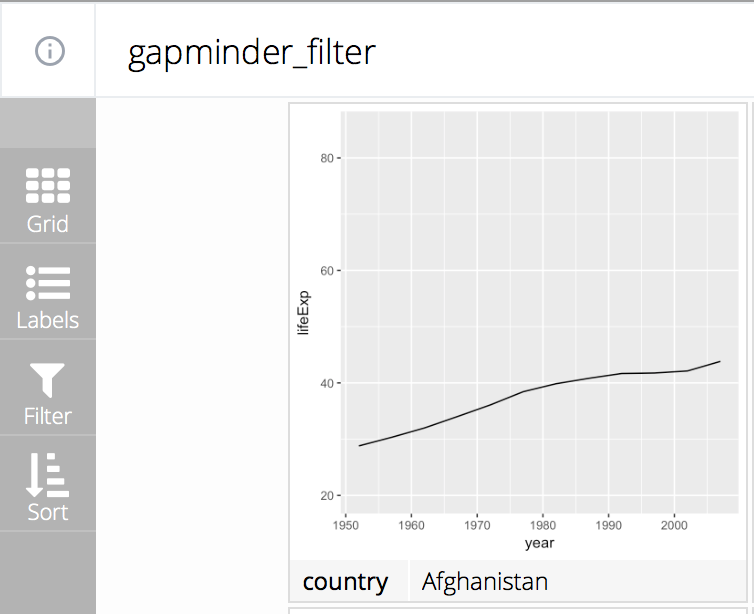
\includegraphics[height=2.5in]{./figs/tjs_sidebar.png}
  \caption{The sidebar on the left side of a \trelliscopejs~HTML widget can be opened for panel layout control, displaying panel labels, filtering panels, and sorting panels.}
\end{figure}



\section{Cognostics}

Displaying panels alone has already been solved with \ggplot~and \pkg{lattice}.  Scaling panels beyond \pkg{lattice}'s limits is still limited without the use of sorting and filtering the panels.  \trelliscopejs's power is leveraging subset metrics to organize the panels.  These subset metrics are called \emph{cognostics}~\cite{Tukey1985}.  Cognostics are univariate statistics calculated for every independent subset of the conditioned data.

Cognostics can be simple summary statistics such as \rinline{mean} or \rinline{median}, or can be meta data information such as a URL or census information for a conditioned county.  Tukey and Tukey first proposed calculating univariate metrics for scatterplots called scagnostics~\cite{Tukey1985} as a way to describe a scatterplot.  Wilkinson et. al.~\cite{scagnostics} implemented Tukeys' scagnostic definitions in the R package \pkg{scagnostics}~\cite{r_scagnostics}. Scagnostics can be repurposed as cognostics when applied to every panel containing a scatterplot.  These cognostic groupings may then be shown, filtered, and sorted accross the different subset panels.

In \trelliscopejs, cognostics are displayed as two types of metrics: continuous or discrete.  Continuous valued cognostics are filtered using open or closed ranges.  Figure~\ref{fig:gap_seventy} shows an open range using the \rinline{gapminder} country panels that contain a maximum life expectancy value less than or equal to 70 years of age.  A closed range example would have both a \emph{from} and a \emph{to} in the selection range, i.e. within 50 to 65 years of age. Currently, \trelliscopejs~does not support more than one range selection for each cognostic variable.

\begin{figure}[H]
  \label{fig:gap_seventy}
  \centering
  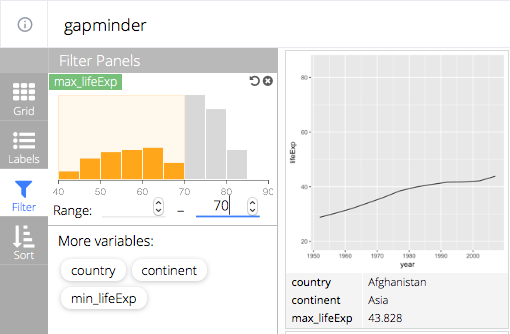
\includegraphics[height=2.5in]{./figs/tjs_filter_70.png}
  \caption{A cropped view of \trelliscopejs~filtering on countries whose maximum life expectancy is lower than 70 years old.}
\end{figure}


With \trelliscopejs, discrete values are handled using regular expressions or by manually selecting values.  When using regular expressions, matching values are displayed immediately.  Figure~\ref{fig:gap_regex} displays the immedate results of regular expression on a continent.  The immediate feedback confirms whether the regular expression was successful or needs to be updated.

\begin{figure}[H]
  \label{fig:gap_regex}
  \centering
  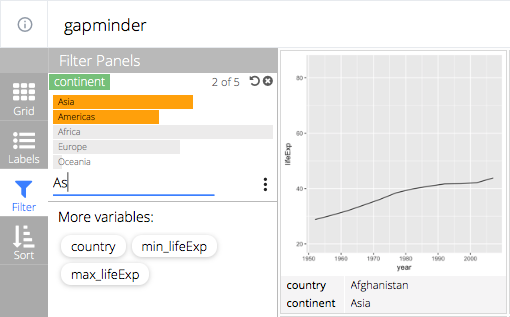
\includegraphics[height=2.5in]{./figs/tjs_filter_as.png}
  \caption{A cropped view of \trelliscopejs~filtering on continent who matches the regular expression ``as''.}
\end{figure}


Multiple filters are a part of the data analysis process and are embraced in \trelliscopejs.  All of the cognostic filters are applied as a collective, logical \emph{and}.

% \trelliscopejs~allows for cognostics to be any univariate value.  This may also include a URL.  While filtering is not effective for a URL, linking to external websites for a particular panel can be useful.  For example, when looking at the housing sales for every county in the United States, a URL can be linked to the website Zillow that displays all current housing sales on the Zillow website for that particular county.

\section{Automatic cognostics for data visualization}

From a data plotting perspective, we should be able to utilize what is already being displayed in the plot to sort and filter the panels of a \trelliscopejs~widget.  This plot information is not readily available as it is calculated within each plotting mechanism.

Using the prior \trelliscopejs~example in Figure~\ref{fig:trelliscopejs_two}, the minimum and maximum values for each country's life expectancy were calculated manually.  While the prior example only retrieved the minimum and maximum life expectancy values for each panel, the median and mean values may be of interest as well. These statistics are only looking at the $Y$ variable.  There are many more statistics involving both the $Y$ variable and the $X$ variable.  In Figure~\ref{fig:add_metrics}, the $X$ and $Y$ covariance and correlation are added.  A linear model (\rinline{geom_smooth(method = "lm")}) is also added to visually detect linear trend deviations.

\begin{knitrout}\small
\definecolor{shadecolor}{rgb}{0.969, 0.969, 0.969}\color{fgcolor}\begin{kframe}
\begin{alltt}
\hlstd{gapminder_condensed} \hlopt
  \hlkwd{mutate}\hlstd{(}
    \hlcom{# add metrics}
    \hlkwc{min_lifeExp} \hlstd{= purrr}\hlopt{::}\hlkwd{map_dbl}\hlstd{(data,} \hlkwa{function}\hlstd{(}\hlkwc{dt}\hlstd{)} \hlkwd{min}\hlstd{(dt}\hlopt{$}\hlstd{lifeExp)),}
    \hlkwc{mean_lifeExp} \hlstd{= purrr}\hlopt{::}\hlkwd{map_dbl}\hlstd{(data,} \hlkwa{function}\hlstd{(}\hlkwc{dt}\hlstd{)} \hlkwd{mean}\hlstd{(dt}\hlopt{$}\hlstd{lifeExp)),}
    \hlkwc{median_lifeExp} \hlstd{= purrr}\hlopt{::}\hlkwd{map_dbl}\hlstd{(data,} \hlkwa{function}\hlstd{(}\hlkwc{dt}\hlstd{)} \hlkwd{median}\hlstd{(dt}\hlopt{$}\hlstd{lifeExp)),}
    \hlkwc{max_lifeExp} \hlstd{= purrr}\hlopt{::}\hlkwd{map_dbl}\hlstd{(data,} \hlkwa{function}\hlstd{(}\hlkwc{dt}\hlstd{)} \hlkwd{max}\hlstd{(dt}\hlopt{$}\hlstd{lifeExp)),}
    \hlkwc{cov} \hlstd{= purrr}\hlopt{::}\hlkwd{map_dbl}\hlstd{(data,} \hlkwa{function}\hlstd{(}\hlkwc{dt}\hlstd{)} \hlkwd{cov}\hlstd{(dt}\hlopt{$}\hlstd{year, dt}\hlopt{$}\hlstd{lifeExp)),}
    \hlkwc{corr} \hlstd{= purrr}\hlopt{::}\hlkwd{map_dbl}\hlstd{(data,} \hlkwa{function}\hlstd{(}\hlkwc{dt}\hlstd{)} \hlkwd{cor}\hlstd{(dt}\hlopt{$}\hlstd{year, dt}\hlopt{$}\hlstd{lifeExp)),}

    \hlcom{# add panel}
    \hlkwc{panel} \hlstd{= trelliscopejs}\hlopt{::}\hlkwd{map_plot}\hlstd{(data,} \hlkwa{function}\hlstd{(}\hlkwc{dt}\hlstd{) \{}
      \hlcom{# display a line plot of X:year, Y:life expectancy}
      \hlkwd{ggplot}\hlstd{(dt,} \hlkwd{aes}\hlstd{(year, lifeExp))} \hlopt{+}
        \hlkwd{geom_smooth}\hlstd{(}\hlkwc{method} \hlstd{=} \hlstr{"lm"}\hlstd{)} \hlopt{+} \hlcom{# add a linear model}
        \hlkwd{geom_line}\hlstd{()} \hlopt{+}
        \hlkwd{ylim}\hlstd{(}\hlnum{20}\hlstd{,} \hlnum{85}\hlstd{)}
    \hlstd{\})}
  \hlstd{)} \hlopt
  \hlcom{# remove the condensed data}
  \hlkwd{select}\hlstd{(}\hlopt{-}\hlstd{data)} \hlopt
  \hlkwd{print}\hlstd{()} \hlkwb{->}
\hlstd{gap_trellis_plus}
\end{alltt}
\begin{verbatim}
## # A tibble: 142 x 9
##        country continent min_lifeExp mean_lifeExp median_lifeExp
##         <fctr>    <fctr>       <dbl>        <dbl>          <dbl>
##  1 Afghanistan      Asia      28.801     37.47883        39.1460
##  2     Albania    Europe      55.230     68.43292        69.6750
##  3     Algeria    Africa      43.077     59.03017        59.6910
##  4      Angola    Africa      30.015     37.88350        39.6945
##  5   Argentina  Americas      62.485     69.06042        69.2115
##  6   Australia   Oceania      69.120     74.66292        74.1150
##  7     Austria    Europe      66.800     73.10325        72.6750
##  8     Bahrain      Asia      50.939     65.60567        67.3225
##  9  Bangladesh      Asia      37.484     49.83408        48.4660
## 10     Belgium    Europe      68.000     73.64175        73.3650
## # ... with 132 more rows, and 4 more variables: max_lifeExp <dbl>,
## #   cov <dbl>, corr <dbl>, panel <list>
\end{verbatim}
\begin{alltt}
\hlstd{gap_trellis_plus} \hlopt \hlkwd{trelljs}\hlstd{(}\hlstr{"gapminder_plus"}\hlstd{)}
\end{alltt}


{\ttfamily\noindent\bfseries\color{errorcolor}{\#\# Error in file(con, "{}r"{}): cannot open the connection}}\end{kframe}
\end{knitrout}

The amount of work to retrieve information that can be readily seen or calculated from the visual display quickly increases.  At first, there were two values used.  Now there are six values used to explain just the $Y$ data and the $\left\{X,Y\right\}$ combination.  None of the added metrics explain the linear model added to each panel.  As the amount of layers increase, the number of cognostics needed to explain the plot layer will also increase.  Given each plotting panel already contains many statistical cognostics, each panel should be leveraged to generate cognostics automatically.



\subsection{Linear model example}
\label{subsec:linear_model}


Using the panel column only, we will automatically derive many cognostics from each panel using the \autocogs~R package.

\begin{knitrout}\small
\definecolor{shadecolor}{rgb}{0.969, 0.969, 0.969}\color{fgcolor}\begin{kframe}
\begin{alltt}
\hlstd{gapminder} \hlopt
  \hlkwd{group_by}\hlstd{(country, continent)} \hlopt
  \hlstd{tidyr}\hlopt{::}\hlkwd{nest}\hlstd{()} \hlopt
  \hlkwd{mutate}\hlstd{(}
    \hlkwc{panel} \hlstd{= trelliscopejs}\hlopt{::}\hlkwd{map_plot}\hlstd{(data,} \hlkwa{function}\hlstd{(}\hlkwc{dt}\hlstd{) \{}
      \hlcom{# display a line plot of X:year, Y:life expectancy}
      \hlkwd{ggplot}\hlstd{(dt,} \hlkwd{aes}\hlstd{(year, lifeExp))} \hlopt{+}
        \hlkwd{geom_smooth}\hlstd{(}\hlkwc{method} \hlstd{=} \hlstr{"lm"}\hlstd{)} \hlopt{+}
        \hlkwd{geom_line}\hlstd{()} \hlopt{+}
        \hlkwd{ylim}\hlstd{(}\hlnum{20}\hlstd{,} \hlnum{85}\hlstd{)}
    \hlstd{\})}
  \hlstd{)} \hlopt
  \hlkwd{select}\hlstd{(}\hlopt{-}\hlstd{data)} \hlopt \hlcom{# remove the condensed data}
  \hlkwd{print}\hlstd{()} \hlkwb{->}
\hlstd{gap_panel}
\end{alltt}
\begin{verbatim}
## # A tibble: 142 x 3
##        country continent    panel
##         <fctr>    <fctr>   <list>
##  1 Afghanistan      Asia <S3: gg>
##  2     Albania    Europe <S3: gg>
##  3     Algeria    Africa <S3: gg>
##  4      Angola    Africa <S3: gg>
##  5   Argentina  Americas <S3: gg>
##  6   Australia   Oceania <S3: gg>
##  7     Austria    Europe <S3: gg>
##  8     Bahrain      Asia <S3: gg>
##  9  Bangladesh      Asia <S3: gg>
## 10     Belgium    Europe <S3: gg>
## # ... with 132 more rows
\end{verbatim}
\begin{alltt}
\hlstd{autocogs}\hlopt{::}\hlkwd{add_panel_cogs}\hlstd{(gap_panel)}
\end{alltt}
\begin{verbatim}
## # A tibble: 142 x 9
##        country continent    panel        `_smooth`             `_lm`
##         <fctr>    <fctr>   <list>           <list>            <list>
##  1 Afghanistan      Asia <S3: gg> <tibble [1 x 3]> <tibble [1 x 19]>
##  2     Albania    Europe <S3: gg> <tibble [1 x 3]> <tibble [1 x 19]>
##  3     Algeria    Africa <S3: gg> <tibble [1 x 3]> <tibble [1 x 19]>
##  4      Angola    Africa <S3: gg> <tibble [1 x 3]> <tibble [1 x 19]>
##  5   Argentina  Americas <S3: gg> <tibble [1 x 3]> <tibble [1 x 19]>
##  6   Australia   Oceania <S3: gg> <tibble [1 x 3]> <tibble [1 x 19]>
##  7     Austria    Europe <S3: gg> <tibble [1 x 3]> <tibble [1 x 19]>
##  8     Bahrain      Asia <S3: gg> <tibble [1 x 3]> <tibble [1 x 19]>
##  9  Bangladesh      Asia <S3: gg> <tibble [1 x 3]> <tibble [1 x 19]>
## 10     Belgium    Europe <S3: gg> <tibble [1 x 3]> <tibble [1 x 19]>
## # ... with 132 more rows, and 4 more variables: `_x` <list>,
## #   `_y` <list>, `_bivar` <list>, `_n` <list>
\end{verbatim}
\end{kframe}
\end{knitrout}

For each panel, \rinline{2 + 19 + 5 + 5 + 2 + 5 = 38} cognostics were auto generated to aid in exploration of the panels.

  \begin{itemize}
    \item Ten of the cognostics calculate information individual column information. (\rinline{_x}, \rinline{_y})
    \item Two cognostics calculate continuous bivariate metrics. (\rinline{_bivar})
    \item Five cognostics calculate metrics involving the number of points and their availbility. (\rinline{_n})
    \item Two cognostics calculate metrics for the smooth line added to each panel. (\rinline{_smooth})
    \item Nineteen cognostics are calculated for the linear model applied to the panel.  These metrics will be dicussed in greater detail later. (\rinline{_lm})
  \end{itemize}

Each univariate grouping is labeled to provide context as to what is calculated and which variables were used.


\subsection{Framework}

\autocogs~package is built to provide a consistent framework for calculating cognostics independent of the class of the plotting object supplied.  Ideally, it should work for all major layer-based visualization packages (such as \ggplot, \pkg{rbokeh}~\cite{r_bokeh}, and \pkg{plotly}~\cite{r_plotly}) and produce the same result for similar plot displayed in the different plotting packages.  Currently, only \ggplot~hooks have been installed, but \pkg{rbokeh}~and \pkg{plotly}~can be added using the publically available functions in the \autocogs~package.


By definition, each subset panel within a \trelliscopejs~widget will contain the same plotting layers, but with different data.  Addressing each layer will produce the same group of output cognostics but with different values.  There is a ``one to many'' mapping from plot to plot layers and a ``one to many'' mapping from each plot layer to the cognostic groups.  The same final cognostics may be produced from many different layers as shown in Figure~\ref{fig:cog_fig_layer}.

\begin{figure}[H]
  \label{fig:cog_fig_layer}
  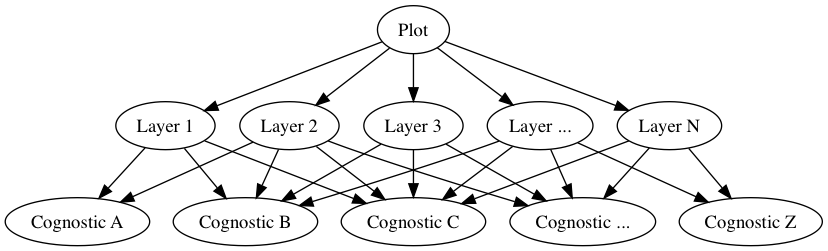
\includegraphics[width = \textwidth ]{./dot/plot_layers.png}
  \caption{Theoretical framework of how multiple cognostic groups can be connected to multiple plot layers.}
\end{figure}

Once all the cognostics have been produced for a given plot, the cognostic groups are reduced to keep only the unique cognostic name and value combinations.  Using Figure~\ref{fig:cog_fig_layer}, the cognostic groups $\left\{A, B, ..., M\right\}$ will only be returned once.











\subsection{Cognostic groups}

Each set of cognostics is returned in a cognostic group.  This is similar to scagnostics.  All scagnostics pertain to scatterplots.  Likewise, the number of non-NA $X$, non-NA $Y$, and non-NA $X$ and $Y$ points pertain to non-NA counts of the displayed data.  These groups can be extended to each type of statistical display: box plot, histogram, linear model, etc.

The cognostics produced in the \autocogs~\rinline{gapminder} linear model example in subsection~\ref{subsec:linear_model} were:
\begin{itemize}
  \item \rinline{_smooth}: Two cognostics pertaining to a ``smooth'' line being added to the panel.
  \item \rinline{_lm}: Nineteen cognostics pertaining to the linear model line added to the panel.
  \item \rinline{_x, _y} Five cognostics pertaining only to the X and Y values respectively.
  \item \rinline{_bivar} Two cognostics pertaining only to both the X and Y values.
  \item \rinline{_n} Five cognostics pertaining only to counts of X and Y values.
\end{itemize}

Each cognostic group column contains a single row \rinline{data.frame} nested in each cell.  Nesting data structures as list-columns~\cite{r4ds} is considered an advanced R technique, but by nesting the cognostic \rinline{data.frame}s in each cell, \autocogs~maintains the tidy data input with tidy data cognostics.  Tidy data is defined to have variables in each column, observations for each row and each cell contains a value.  The value does not need to conform to atomic values which allows for complex structures as long as the ``tidy data'' rules are maintained as shown in Figure~\ref{fig:tidy_data}.


\begin{figure}[H]
  \label{fig:tidy_data}
  \centering
  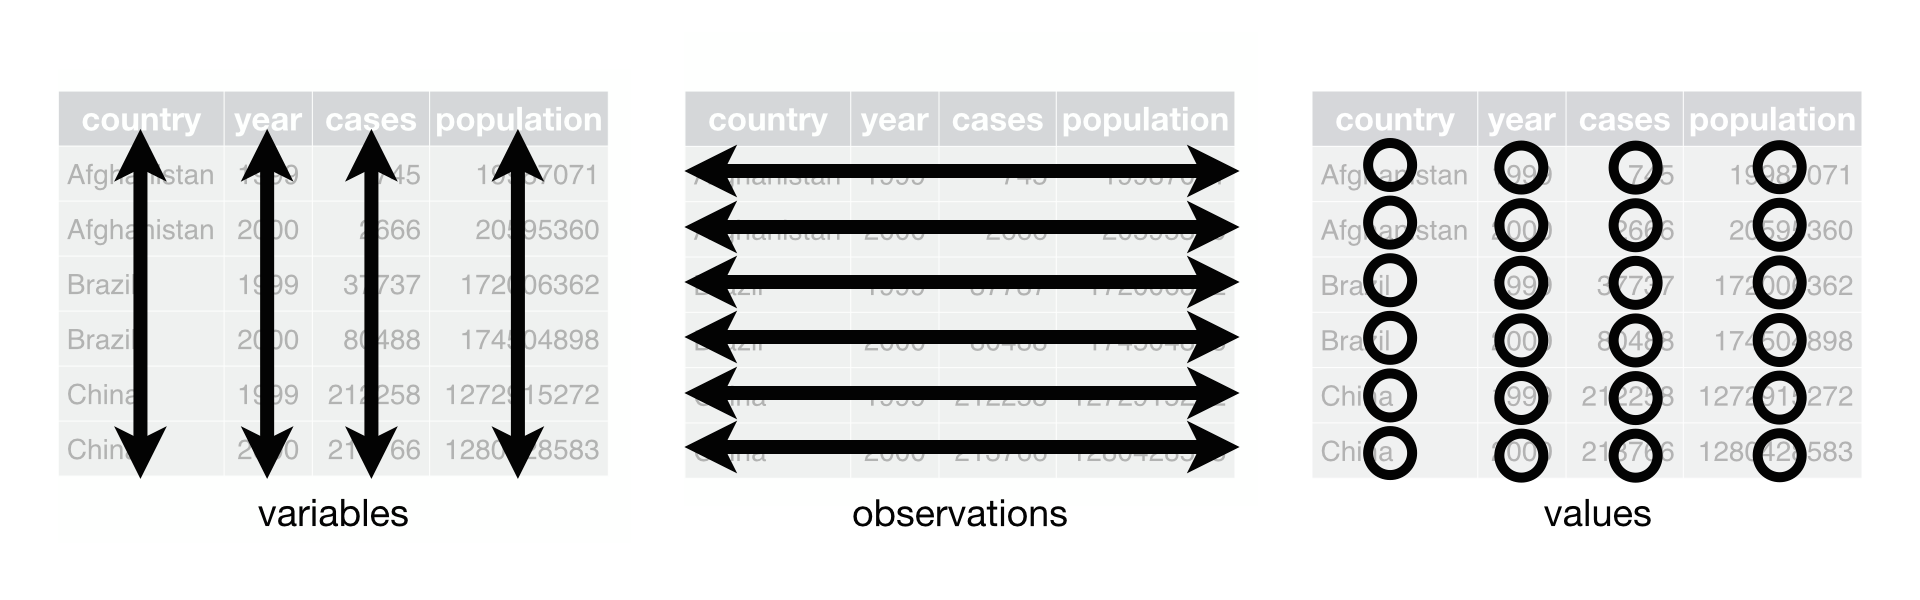
\includegraphics[width=0.9\textwidth]{figs/tidy.png}
  \caption{Figure courtesy of~\cite{r4ds}. There are three rules to tidy data: columns contain variables, rows contain observations, and cells contain values.}
\end{figure}












\section{Cognostic groups}

There are three main types of cognostic groups: Univariate, Bivariate, and Counts.  Each type of cognostic group will explain in detail their corresponding cognostic groups in detail throughout this section.

\subsection{Univariate}

The univariate cognostic groups examples will use the same data set of the maximum life expectancy of the \rinline{gapminder} data set.

\begin{knitrout}\small
\definecolor{shadecolor}{rgb}{0.969, 0.969, 0.969}\color{fgcolor}\begin{kframe}
\begin{alltt}
\hlstd{gapminder} \hlopt
  \hlkwd{group_by}\hlstd{(country, continent)} \hlopt
  \hlkwd{summarise}\hlstd{(}\hlkwc{lifeExp} \hlstd{=} \hlkwd{max}\hlstd{(lifeExp))} \hlopt
  \hlkwd{print}\hlstd{()} \hlkwb{->}
\hlstd{gap_max}
\end{alltt}
\begin{verbatim}
## # A tibble: 142 x 3
## # Groups:   country [?]
##        country continent lifeExp
##         <fctr>    <fctr>   <dbl>
##  1 Afghanistan      Asia  43.828
##  2     Albania    Europe  76.423
##  3     Algeria    Africa  72.301
##  4      Angola    Africa  42.731
##  5   Argentina  Americas  75.320
##  6   Australia   Oceania  81.235
##  7     Austria    Europe  79.829
##  8     Bahrain      Asia  75.635
##  9  Bangladesh      Asia  64.062
## 10     Belgium    Europe  79.441
## # ... with 132 more rows
\end{verbatim}
\end{kframe}
\end{knitrout}


\subsubsection{Univariate Continuous Cognostics}

  Univariate continuous cognostics utilize the standard statistical calculations: minimum, maximum, mean, median, and variance.  Each value is quickly interpretable and provides a good starting point when filtering panels within a \trelliscopejs~widget.

\begin{knitrout}\small
\definecolor{shadecolor}{rgb}{0.969, 0.969, 0.969}\color{fgcolor}\begin{kframe}
\begin{alltt}
\hlkwd{library}\hlstd{(autocogs)}
\hlkwd{auto_cog}\hlstd{(}\hlstr{"univariate_continuous"}\hlstd{, gap_max}\hlopt{$}\hlstd{lifeExp)}
\end{alltt}
\begin{verbatim}
## # A tibble: 1 x 5
##      min    max     mean  median      var
##    <dbl>  <dbl>    <dbl>   <dbl>    <dbl>
## 1 42.568 82.603 68.03542 71.9355 116.3098
\end{verbatim}
\end{kframe}
\end{knitrout}

\subsubsection{Univariate Discrete Cognostics}

  Univariate discrete values only have counts and names to determine the cognostics.  The minimum and maximum count values are reported, as well as the mean count value.  For both the minimum and maximum values, a corresponding name is reported alongside the count.  The example below shows that the continent \rinline{"Africa"} contains the most countries at \rinline{52} and \rinline{"Oceania"} contains least amount of countries at \rinline{2} countries.

\begin{knitrout}\small
\definecolor{shadecolor}{rgb}{0.969, 0.969, 0.969}\color{fgcolor}\begin{kframe}
\begin{alltt}
\hlkwd{auto_cog}\hlstd{(}\hlstr{"univariate_discrete"}\hlstd{, gap_max}\hlopt{$}\hlstd{continent)}
\end{alltt}
\begin{verbatim}
## # A tibble: 1 x 5
##   min_name count_min count_mean count_max max_name
##      <chr>     <int>      <dbl>     <int>    <chr>
## 1  Oceania         2       28.4        52   Africa
\end{verbatim}
\end{kframe}
\end{knitrout}

  \subsubsection{Continuous Density Cognostics}

  Continuous density cognostics revolve around the shape of the density.  The maximum density value and its corresponding location are returned for comparison across cognostic calculations. Skew and kurtosis~\cite{casella2002statistical} are computed to help distinguish the density shape.  The p value of Hartigans' dip test from \pkg{diptest}~\cite{r_diptest} for unimodality is reported as well.  To help locate where the maximum density occurs, the maximum density value and location are provided.  Finally, the number of clusters may be calculated using the \pkg{mclust}~\cite{r_mclust_1}~\cite{r_mclust_2} R package.  Cluster calculations are not included by default due to their slower computational speed.


\begin{knitrout}\small
\definecolor{shadecolor}{rgb}{0.969, 0.969, 0.969}\color{fgcolor}\begin{kframe}
\begin{alltt}
\hlkwd{auto_cog}\hlstd{(}\hlstr{"density_continuous"}\hlstd{, gap_max}\hlopt{$}\hlstd{lifeExp,} \hlkwc{clusters} \hlstd{=} \hlnum{TRUE}\hlstd{)}
\end{alltt}
\begin{verbatim}
## # A tibble: 1 x 6
##   max_density max_density_location clusters unimodal_p_value
##         <dbl>                <dbl>    <int>            <dbl>
## 1  0.04425023             75.22066        3        0.2994391
## # ... with 2 more variables: skew <dbl>, kurt <dbl>
\end{verbatim}
\end{kframe}
\end{knitrout}


  \subsubsection{Boxplot Cognostics}

  Boxplot metrics include lower whisker, Q1, median, Q3, and upper whisker locations.  The number of outliers above the boxplot and below the boxplot are also reported.

\begin{knitrout}\small
\definecolor{shadecolor}{rgb}{0.969, 0.969, 0.969}\color{fgcolor}\begin{kframe}
\begin{alltt}
\hlkwd{auto_cog}\hlstd{(}\hlstr{"boxplot"}\hlstd{, gap_max}\hlopt{$}\hlstd{lifeExp)}
\end{alltt}
\begin{verbatim}
## # A tibble: 1 x 7
##   n_outlier_lower lower_whisker       q1  median       q3
##             <int>         <dbl>    <dbl>   <dbl>    <dbl>
## 1               0       59.6945 69.71875 71.9355 74.15225
## # ... with 2 more variables: upper_whisker <dbl>,
## #   n_outlier_upper <int>
\end{verbatim}
\end{kframe}
\end{knitrout}

  \subsubsection{Quantile Quantile Cognostics}

Quantile-Quantile plots display the theoretical distribution quantiles verses the sample quantile points.  Two variables to help determine skewness count how many points are above and below a non robust quantile line.  The non robust quantile line is calculated using the $25^{th}$ and $75^{th}$ percentiles of sample points, rather than the a robust linear model.  This calculation replicates the base R function \rinline{stats::qqline} behavior.  A p value for the Kolmogorov-Smirnov test is added to the result to determine how close the sample points come from the test distribution.  The test distribution defaults to the normal distribution.  Finally, a mean squared error from the quantile line is reported for the Quantile-Quantile plot.  This value should be comparable to all of the independent samples as each sample should come from the same distribution.  Larger mean squared error values help discover outliers in the distribution.

\begin{knitrout}\small
\definecolor{shadecolor}{rgb}{0.969, 0.969, 0.969}\color{fgcolor}\begin{kframe}
\begin{alltt}
\hlkwd{auto_cog}\hlstd{(}\hlstr{"quantile_quantile"}\hlstd{, gap_max}\hlopt{$}\hlstd{lifeExp)}
\end{alltt}
\begin{verbatim}
## # A tibble: 1 x 4
##   points_above points_below ks_test   qq_mse
##          <int>        <int>   <dbl>    <dbl>
## 1           87           55       0 13.78215
\end{verbatim}
\end{kframe}
\end{knitrout}



\subsection{Bivariate}

The cognostic groups below is calculated using the \rinline{gapminder} data set where continent equals \rinline{"Americas"} (\rinline{americas}) or where country equals \rinline{"United States"} (\rinline{usa}).

\begin{knitrout}\small
\definecolor{shadecolor}{rgb}{0.969, 0.969, 0.969}\color{fgcolor}\begin{kframe}
\begin{alltt}
\hlstd{americas} \hlkwb{<-} \hlstd{gapminder} \hlopt \hlkwd{filter}\hlstd{(continent} \hlopt{==} \hlstr{"Americas"}\hlstd{)}
\hlstd{usa} \hlkwb{<-} \hlstd{gapminder} \hlopt \hlkwd{filter}\hlstd{(country} \hlopt{==} \hlstr{"United States"}\hlstd{)}
\end{alltt}
\end{kframe}
\end{knitrout}

  \subsubsection{Bivariate Continuous Cognostics}

Similar to the Univariate Continuous cognostic group, the Bivariate Continuous cognostic group calculates the two standard bivariate summary statistics: covariance and correlation.

\begin{knitrout}\small
\definecolor{shadecolor}{rgb}{0.969, 0.969, 0.969}\color{fgcolor}\begin{kframe}
\begin{alltt}
\hlkwd{auto_cog}\hlstd{(}\hlstr{"bivariate_continuous"}\hlstd{, usa}\hlopt{$}\hlstd{year, usa}\hlopt{$}\hlstd{lifeExp)}
\end{alltt}
\begin{verbatim}
## # A tibble: 1 x 2
##   covariance correlation
##        <dbl>       <dbl>
## 1     59.855   0.9929351
\end{verbatim}
\end{kframe}
\end{knitrout}

\subsubsection{Scagnostics Cognostics}

Scatterplot scagnostics are a pre-existing cognostic group for a continuous bivariate plot. The following scagnostics are explained in more detail in~\cite{scagnostics}.

\begin{itemize}
  \item Outlying: the proportion of the total edge length due to extremely long edges connected to points of single degree.
  \item Skewed: the distribution of edge lengths of a minimum spanning tree gives us information about the relative density of points in a scattered configuration.
  \item Clumpy: the Hartigan and Mohanty RUNT statistic is most easily understood in terms of the single-linkage hierarchical clustering tree called a dendrogram.
  \item Sparse, the 90\% quantile of the edge lengths of the minimum spanning tree.
  \item Striated: the summation of angles over all adjacent edges of a MST.
  \item Convex: the ratio of the area of the alpha hull and the area of the convex hull.
  \item Skinny: the ratio of perimeter to area of a polygon measures.
  \item Stringy: the ratio of width to length of a network.
  \item Monotonic: squared Spearman correlation coefficient.
\end{itemize}

\begin{knitrout}\small
\definecolor{shadecolor}{rgb}{0.969, 0.969, 0.969}\color{fgcolor}\begin{kframe}
\begin{alltt}
\hlkwd{auto_cog}\hlstd{(}\hlstr{"scagnostics"}\hlstd{, americas}\hlopt{$}\hlstd{year, americas}\hlopt{$}\hlstd{lifeExp)}
\end{alltt}
\begin{verbatim}
## # A tibble: 1 x 9
##     Outlying    Skewed     Clumpy    Sparse  Striated    Convex
##        <dbl>     <dbl>      <dbl>     <dbl>     <dbl>     <dbl>
## 1 0.01443262 0.7695572 0.07343219 0.0799376 0.5539216 0.8622428
## # ... with 3 more variables: Skinny <dbl>, Stringy <dbl>,
## #   Monotonic <dbl>
\end{verbatim}
\end{kframe}
\end{knitrout}

  \subsubsection{Continuous 2D Density Cognostics}

The Continuous 2-Dimensional Density cognostic group reports the maximum density.  Similar to the Continuous Density cognostic group, the $X$ and $Y$ location are returned.  Cluster count calculations are turned off by default due to slow computation speed.


\begin{knitrout}\small
\definecolor{shadecolor}{rgb}{0.969, 0.969, 0.969}\color{fgcolor}\begin{kframe}
\begin{alltt}
\hlkwd{auto_cog}\hlstd{(}
  \hlstr{"density_2d_continuous"}\hlstd{,}
  \hlstd{americas}\hlopt{$}\hlstd{year, americas}\hlopt{$}\hlstd{lifeExp,}
  \hlkwc{clusters} \hlstd{=} \hlnum{TRUE}
\hlstd{)}
\end{alltt}
\begin{verbatim}
## # A tibble: 1 x 4
##   max_density max_density_x max_density_y clusters
##         <dbl>         <dbl>         <dbl>    <int>
## 1  0.00118169      1997.435      71.86533        9
\end{verbatim}
\end{kframe}
\end{knitrout}

\subsubsection{Bivariate Step Cognostics}

A stepwise plot displays a ``stair case'' like plot where the connecting line only moves in parallel ot the $X$ or $Y$ axis.  The Bivariate Step cognostic group returns the number of steps completed, as well as calculating the Univariate Continuous cognostics for the step width and step height.

\begin{knitrout}\small
\definecolor{shadecolor}{rgb}{0.969, 0.969, 0.969}\color{fgcolor}\begin{kframe}
\begin{alltt}
\hlkwd{auto_cog}\hlstd{(}\hlstr{"bivariate_step"}\hlstd{, usa}\hlopt{$}\hlstd{year, usa}\hlopt{$}\hlstd{lifeExp)}
\end{alltt}
\begin{verbatim}
## # A tibble: 1 x 11
##   steps min_step_width mean_step_width median_step_width
##   <dbl>          <int>           <dbl>             <int>
## 1    11              5               5                 5
## # ... with 7 more variables: max_step_width <int>,
## #   var_step_width <dbl>, min_step_height <dbl>,
## #   mean_step_height <dbl>, median_step_height <dbl>,
## #   max_step_height <dbl>, var_step_height <dbl>
\end{verbatim}
\end{kframe}
\end{knitrout}

\subsubsection{Smooth Line Cognostics}

The Smooth Line cognostic group is a baseline for all model based lines added to a plot.  The smooth line calculations pair well with the Linear Model and Loess Model cognostic groups.  A mean squared error and the max deviation with its corresponding location are reported.

\begin{knitrout}\small
\definecolor{shadecolor}{rgb}{0.969, 0.969, 0.969}\color{fgcolor}\begin{kframe}
\begin{alltt}
\hlkwd{auto_cog}\hlstd{(}\hlstr{"smooth_line"}\hlstd{, usa}\hlopt{$}\hlstd{year, usa}\hlopt{$}\hlstd{lifeExp)}
\end{alltt}
\begin{verbatim}
## # A tibble: 1 x 3
##          mse max_deviation max_deviation_location
##        <dbl>         <dbl>                  <int>
## 1 0.05389673       0.45948                   1972
\end{verbatim}
\end{kframe}
\end{knitrout}


\subsubsection{Linear Model Cognostics}

Linear Model cognostics leverage many existing statistics.  Knowing that the model will only be a simple linear model allows \autocogs~to return slope and intercept values and corresponding p values.  Many cognostics can be generated about the model fit using known diagnostic methods:
  \begin{itemize}
    \item $R^2$: fraction of variance explained by the model
    \item $\sigma$: square root of the estimated residual variance
    \item $F$-statistic: the linear model's $F$-statistic and corresponding p value.
    \item Degrees of freedom: how many degrees of freedom in the model and residuals
    \item Log-likelihood value: the log likelihood value of the model
    \item AIC, BIC: Akaike's Information Criterion and Schwarz's Bayesian Criterion
    \item Deviance: the quality-of-fit statistic of the model
  \end{itemize}

  There are a few extra diagnostics that perform extra calculations to conform to the univariate requirement of a cognostic.

  \begin{itemize}
    \item Cook's distance: a combination of each points leverage and residual value.  Values larger than $F_{p, n - p}(0.5)$ indicate influential data points in the model~\cite{kutner_linear_models}.  The number of influential data points is reported.
    \item Influence points: the diagonal of the Hat Matrix is how much influence a point has on the model.  Each point is expected to equal $\dfrac{p}{n} = \dfrac{1}{n}$, with influential points having a value larger than $\dfrac{2 * p}{n} = \dfrac{2}{n}$~\cite{kutner_linear_models}.  The sum of all influential points is reported.
    \item Shapiro-Wilk test: when using a linear model, the residuals are assumed to come from a normal distribution. The Shapiro-Wilk test tests the residuals against the normal distribution~\cite{kutner_linear_models}.  The corresponding p value is reported.
    \item Box Cox power transformation: the lower and upper bounds of the 95\% confidence interval of the Box Cox power transformation are reported. This transformation is used to  stabilize the variance of a linear model. If the confidence interval contains 0, a $ln$ transformation may be used~\cite{kutner_linear_models}.
  \end{itemize}


\begin{knitrout}\small
\definecolor{shadecolor}{rgb}{0.969, 0.969, 0.969}\color{fgcolor}\begin{kframe}
\begin{alltt}
\hlkwd{auto_cog}\hlstd{(}\hlstr{"linear_model"}\hlstd{, usa}\hlopt{$}\hlstd{year, usa}\hlopt{$}\hlstd{lifeExp)} \hlopt \hlkwd{as.data.frame}\hlstd{()}
\end{alltt}
\begin{verbatim}
##   intercept intercept_p_value      beta beta_p_value        r2
## 1 -291.0845      1.254513e-09 0.1841692 1.369788e-10 0.9859202
##       sigma statistic      p_value           df   log_lik      aic
## 1 0.4161339  700.2351 1.369788e-10 1.369788e-10 -5.412356 16.82471
##        bic deviance df_residual n_sig_cooks n_sig_hat resid_shapiro
## 1 18.27943 1.731675          10           0         6     0.9843222
##   bc_lower bc_upper
## 1     -1.3        2
\end{verbatim}
\end{kframe}
\end{knitrout}

  \subsubsection{Loess Model Cognostics}

  Similar to the linear model, a simple loess model is calculated and the model diagnostics are reported:
  \begin{itemize}
    \item Supplied parameters: the supplied parameters of \rinline{span}, the alpha parameter which controls the degree of smoothing, and \rinline{degree}, the polynomial degree used in the loess model, are returned.
    \item Calculated parameters: the effective number of parameters, \rinline{enp}, is returned along with the trace of the hat matrix, \rinline{trace.hat}.  Finally, the sigma value, \rinline{s}, of the loess model variance is returned as a single cognostic.
    \item Iterations: The number of iterations needed to calculate the model are reported as well.
  \end{itemize}

\begin{knitrout}\small
\definecolor{shadecolor}{rgb}{0.969, 0.969, 0.969}\color{fgcolor}\begin{kframe}
\begin{alltt}
\hlkwd{auto_cog}\hlstd{(}\hlstr{"loess_model"}\hlstd{, usa}\hlopt{$}\hlstd{year, usa}\hlopt{$}\hlstd{lifeExp)}
\end{alltt}
\begin{verbatim}
## # A tibble: 1 x 6
##        enp         s trace.hat  span degree iterations
##      <dbl>     <dbl>     <dbl> <dbl>  <int>      <int>
## 1 4.540734 0.3147398  5.005914  0.75      2          1
\end{verbatim}
\end{kframe}
\end{knitrout}


\subsection{Counts}

The third cognostic type addresses counts of binned data.

  \subsubsection{Univariate and Bivariate Count Cognostics}

  Both the Univariate and Bivariate Count cognostics address how many values are \rinline{NA} and not \rinline{NA}.  Bivariate accounts for both the logical AND and OR of the $X$ and $Y$ values being \rinline{NA}.

\begin{knitrout}\small
\definecolor{shadecolor}{rgb}{0.969, 0.969, 0.969}\color{fgcolor}\begin{kframe}
\begin{alltt}
\hlkwd{auto_cog}\hlstd{(}\hlstr{"univariate_counts"}\hlstd{, americas}\hlopt{$}\hlstd{lifeExp)}
\end{alltt}
\begin{verbatim}
## # A tibble: 1 x 2
##       n  n_na
##   <int> <int>
## 1   300     0
\end{verbatim}
\begin{alltt}
\hlkwd{auto_cog}\hlstd{(}\hlstr{"bivariate_counts"}\hlstd{, americas}\hlopt{$}\hlstd{year, americas}\hlopt{$}\hlstd{lifeExp)}
\end{alltt}
\begin{verbatim}
## # A tibble: 1 x 5
##       n n_both_na n_or_na n_x_na n_y_na
##   <int>     <int>   <int>  <int>  <int>
## 1   300         0       0      0      0
\end{verbatim}
\end{kframe}
\end{knitrout}




\subsubsection{Pairwise Counts Cognostics}

Pairwise Counts cognostics address how often pieces of information occur.  Pairwise Counts look at the combinations of the $X$ and $Y$ variables.  The Univariate Continous cognostics are reported on the counts of the pairwise combinations.
% Pairwise and Grouped Counts cognostics address how often pieces of information occur.  Pairwise Counts look at the combinations of the $X$ and $Y$ variables.  The Univariate Continous Cognostics are reported on the counts of the pairwise combinations.  Grouped Counts provide Univariate Continuous Cognostics for how often a group is used.  This is very similar to Univariate Discrete Cognostics begin applied to the grouping variable only.

\begin{knitrout}\small
\definecolor{shadecolor}{rgb}{0.969, 0.969, 0.969}\color{fgcolor}\begin{kframe}
\begin{alltt}
\hlkwd{auto_cog}\hlstd{(}\hlstr{"pairwise_counts"}\hlstd{, americas}\hlopt{$}\hlstd{country,} \hlkwd{round}\hlstd{(americas}\hlopt{$}\hlstd{lifeExp))}
\end{alltt}
\begin{verbatim}
## # A tibble: 1 x 6
##     min   max     mean median       var na_count
##   <int> <int>    <dbl>  <int>     <dbl>    <dbl>
## 1     1     4 1.083032      1 0.1198922        0
\end{verbatim}
\end{kframe}
\end{knitrout}
% auto_cog("grouped_counts", gap_max$country, gap_max$continent)

\subsubsection{Count Testing Cognostics}

  There are three types of count testing cognostic groupings.  In addition to the Univariate Continuous cognostic information, each cognostic group tests whether or not the variables involved in the plot have any effect on the number of counts.  This is calculated using a $\chi^2$ test where $H_0 = Y ~ \mu$.

  \begin{itemize}

    \item Histogram Counts Cognostics

    The univariate case calculates the counts of a histogram using a default binwidth of 30 equal bin widths.  The default width of 30 matches the default width in \ggplot.

% << echo = FALSE, verbose = FALSE, cache = FALSE >>=
% options(width = 64)
% @
\begin{knitrout}\small
\definecolor{shadecolor}{rgb}{0.969, 0.969, 0.969}\color{fgcolor}\begin{kframe}
\begin{alltt}
\hlkwd{auto_cog}\hlstd{(}\hlstr{"histogram_counts"}\hlstd{, americas}\hlopt{$}\hlstd{lifeExp)}
\end{alltt}
\begin{verbatim}
## # A tibble: 1 x 6
##   count_min count_max count_mean count_median count_var        chisq
##       <dbl>     <dbl>      <dbl>        <dbl>     <dbl>        <dbl>
## 1         0        26         10            8  55.24138 4.240986e-20
\end{verbatim}
\end{kframe}
\end{knitrout}

    \item Square Counts Cognostics

    The bivariate case of the histogram is a 2D square grid.  The counts in each of the grid spaces are calculated using a default binwidth of 30 equal intervals along each axis.  In the example below, six equally spaced bins along each axis are used.

\begin{knitrout}\small
\definecolor{shadecolor}{rgb}{0.969, 0.969, 0.969}\color{fgcolor}\begin{kframe}
\begin{alltt}
\hlkwd{auto_cog}\hlstd{(}
  \hlstr{"square_counts"}\hlstd{,}
  \hlstd{americas}\hlopt{$}\hlstd{year, americas}\hlopt{$}\hlstd{lifeExp,}
  \hlkwc{bins} \hlstd{=} \hlnum{6}
\hlstd{)}
\end{alltt}
\begin{verbatim}
## # A tibble: 1 x 6
##   count_min count_max count_mean count_median count_var        chisq
##       <dbl>     <dbl>      <dbl>        <dbl>     <dbl>        <dbl>
## 1         1        29      9.375          6.5  53.79032 1.547182e-22
\end{verbatim}
\end{kframe}
\end{knitrout}

    \item Hexagon Counts Cognostics

    The second bivariate histogram has a honeycomb like array of hexagons.  Like the Square Counts Cognostics, the Hexagon Counts Cognostics default to 30 equally spaced hexagons along each axis.  The example below also uses six hexagon shaped bins along each axis.

\begin{knitrout}\small
\definecolor{shadecolor}{rgb}{0.969, 0.969, 0.969}\color{fgcolor}\begin{kframe}
\begin{alltt}
\hlkwd{auto_cog}\hlstd{(}\hlstr{"hex_counts"}\hlstd{, americas}\hlopt{$}\hlstd{year, americas}\hlopt{$}\hlstd{lifeExp,} \hlkwc{bins} \hlstd{=} \hlnum{6}\hlstd{)}
\end{alltt}
\begin{verbatim}
## # A tibble: 1 x 6
##   count_min count_max count_mean count_median count_var        chisq
##       <dbl>     <dbl>      <dbl>        <dbl>     <dbl>        <dbl>
## 1         1        25   7.894737            6  38.04267 2.131691e-20
\end{verbatim}
\end{kframe}
\end{knitrout}
% << echo = FALSE, verbose = FALSE, cache = FALSE >>=
% options(width = 69)
% @



  \end{itemize}




\section{\ggplot~layer matching}

\ggplot~has already been integrated into the \autocogs~R package.  This integration contains the mapping of each cognostic group to each \ggplot~geom layer.  Each plotting framework has its own data personality and may display cognostics how it sees fit.

Figure~\ref{fig:geom_mapping} is a mapping of each \ggplot~geom layer to each of the univariate cognostics.  Geoms that do not map to any cognostic groups are considered building block geoms and do not produce any cognostics when added as a layer.

\begin{figure}
  \label{fig:geom_mapping}
  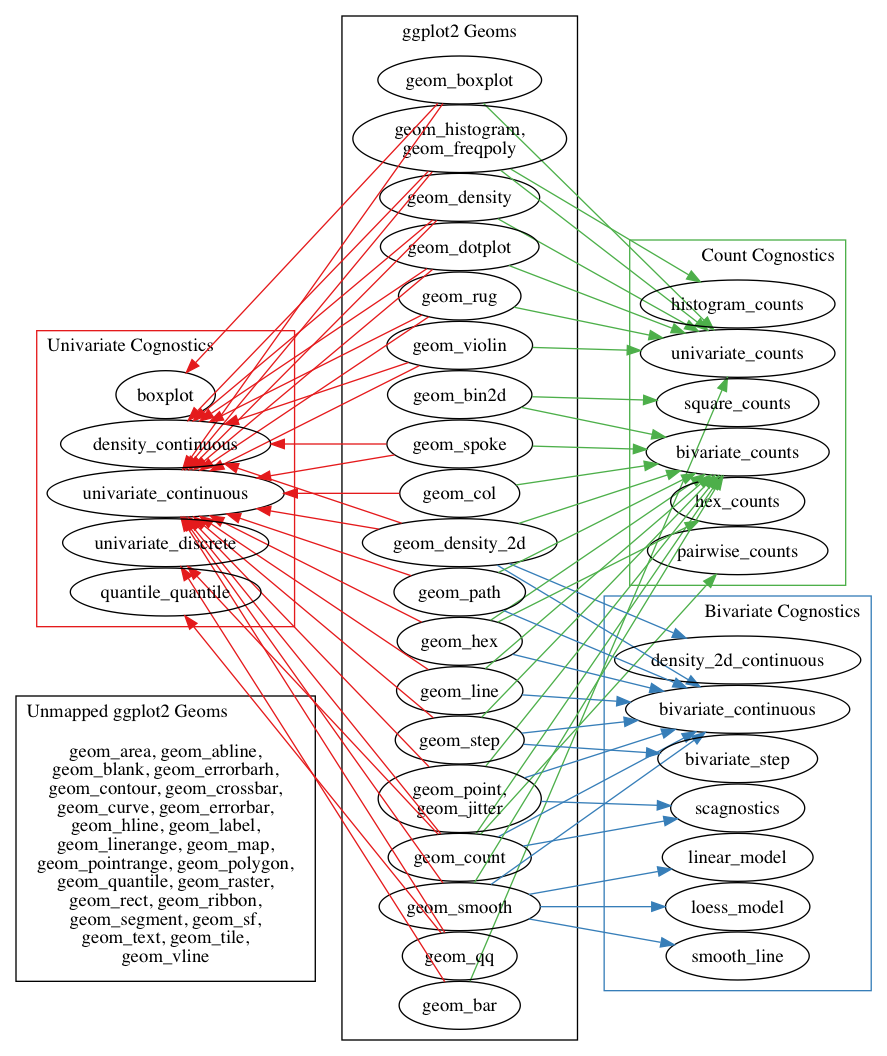
\includegraphics[width=\textwidth]{./dot/ggplot_cognostics.png}
  \caption{Mapping of \ggplot~geoms to Univariate, Bivariate, and Count cognostic groups}
\end{figure}




In this section, I will explore a simple \ggplot~histogram and a more advanced example involving a \ggplot~scatterplot and linear model.

\subsection{Histogram}

First, let us create the data set containing each of the panels.  Each panel will display a histogram chart of the life expectancy over time for each continent. Figure~\ref{fig:continent_hist} displays the panel where continent is equal to \rinline{"Americas"}.

\begin{knitrout}\small
\definecolor{shadecolor}{rgb}{0.969, 0.969, 0.969}\color{fgcolor}\begin{kframe}
\begin{alltt}
\hlstd{gapminder} \hlopt
  \hlkwd{group_by}\hlstd{(continent)} \hlopt
  \hlkwd{do}\hlstd{(}
    \hlkwc{panel} \hlstd{=} \hlkwd{ggplot}\hlstd{(.,} \hlkwd{aes}\hlstd{(lifeExp))} \hlopt{+} \hlkwd{geom_histogram}\hlstd{(}\hlkwc{binwidth} \hlstd{=} \hlnum{1}\hlstd{)}
  \hlstd{)} \hlopt
  \hlkwd{print}\hlstd{()} \hlkwb{->}
\hlstd{continent_hists}
\end{alltt}
\begin{verbatim}
## Source: local data frame [5 x 2]
## Groups: <by row>
## 
## # A tibble: 5 x 2
##   continent    panel
## *    <fctr>   <list>
## 1    Africa <S3: gg>
## 2  Americas <S3: gg>
## 3      Asia <S3: gg>
## 4    Europe <S3: gg>
## 5   Oceania <S3: gg>
\end{verbatim}
\begin{alltt}
\hlstd{americas_pos} \hlkwb{<-} \hlkwd{which}\hlstd{(continent_hists}\hlopt{$}\hlstd{continent} \hlopt{==} \hlstr{"Americas"}\hlstd{)}
\hlstd{continent_hists}\hlopt{$}\hlstd{panel[[americas_pos]]}
\end{alltt}
\end{kframe}\begin{figure}[H]

{\centering \includegraphics[width=4in,height=3in]{figure/continent_hist-1} 

}

\caption{The \rinline{"Americas"} histogram of life expectancy.}\label{fig:continent_hist}
\end{figure}


\end{knitrout}

With a nested \rinline{data.frame} full of panels, we add the cognostics to the \rinline{data.frame}.

\begin{knitrout}\small
\definecolor{shadecolor}{rgb}{0.969, 0.969, 0.969}\color{fgcolor}\begin{kframe}
\begin{alltt}
\hlstd{continent_hists_cogs} \hlkwb{<-} \hlstd{autocogs}\hlopt{::}\hlkwd{add_panel_cogs}\hlstd{(continent_hists)} \hlopt
  \hlkwd{print}\hlstd{()}
\end{alltt}
\begin{verbatim}
## Source: local data frame [5 x 6]
## Groups: <by row>
## 
## # A tibble: 5 x 6
##   continent    panel             `_x`     `_density_x`
##      <fctr>   <list>           <list>           <list>
## 1    Africa <S3: gg> <tibble [1 x 5]> <tibble [1 x 6]>
## 2  Americas <S3: gg> <tibble [1 x 5]> <tibble [1 x 6]>
## 3      Asia <S3: gg> <tibble [1 x 5]> <tibble [1 x 6]>
## 4    Europe <S3: gg> <tibble [1 x 5]> <tibble [1 x 6]>
## 5   Oceania <S3: gg> <tibble [1 x 5]> <tibble [1 x 6]>
## # ... with 2 more variables: `_hist_x` <list>, `_n` <list>
\end{verbatim}
\begin{alltt}
\hlkwd{as.list}\hlstd{(continent_hists_cogs[americas_pos,} \hlnum{3}\hlopt{:}\hlnum{6}\hlstd{])}
\end{alltt}
\begin{verbatim}
## $`_x`
## $`_x`[[1]]
## # A tibble: 1 x 5
##      min    max     mean median      var
##    <dbl>  <dbl>    <dbl>  <dbl>    <dbl>
## 1 37.579 80.653 64.65874 67.048 87.33067
## 
## 
## $`_density_x`
## $`_density_x`[[1]]
## # A tibble: 1 x 6
##   max_density max_density_location clusters unimodal_p_value
##         <dbl>                <dbl>    <lgl>            <dbl>
## 1  0.04992932             70.13661       NA        0.9927842
## # ... with 2 more variables: skew <dbl>, kurt <dbl>
## 
## 
## $`_hist_x`
## $`_hist_x`[[1]]
## # A tibble: 1 x 6
##   count_min count_max count_mean count_median count_var        chisq
##       <dbl>     <dbl>      <dbl>        <dbl>     <dbl>        <dbl>
## 1         0        18   6.818182            6  25.78013 8.513837e-16
## 
## 
## $`_n`
## $`_n`[[1]]
## # A tibble: 1 x 2
##       n  n_na
##   <int> <int>
## 1   300     0
\end{verbatim}
\end{kframe}
\end{knitrout}

The above R output contains all cognostic groups that apply to a univariate histogram.  For a \ggplot~histogram, \autocogs~creates:
\begin{itemize}
  \item \rinline{`_x`}: univariate continuous cognostics using the $X$ data,
  \item \rinline{`_density_x`}: continuous density cognostics using the $X$ data,
  \item \rinline{`_hist_x`}: histogram counts cognostics using the $X$ data,
  \item \rinline{`_n`}: and univariate count information using the $X$ data.
\end{itemize}

While this amount of information is a little overwhelming, keep in mind the goal of the \autocogs~R package is to provide as many ways to filter and sort data that normally must be calculated manually.  \autocogs~computes cognostics that are suited to each type of visualization layer.


\subsection{Linear model and scatterplot}

In the next example, we will perform a similar workflow, but the panel will contain two layers: points and a linear model line.  Each layer is derived from the same original data, but will help produce a different sets of cognostics.

\begin{knitrout}\small
\definecolor{shadecolor}{rgb}{0.969, 0.969, 0.969}\color{fgcolor}\begin{kframe}
\begin{alltt}
\hlstd{gapminder} \hlopt
  \hlkwd{group_by}\hlstd{(country, continent)} \hlopt
  \hlkwd{do}\hlstd{(}
    \hlkwc{panel} \hlstd{=} \hlkwd{ggplot}\hlstd{(.,} \hlkwd{aes}\hlstd{(year, lifeExp))} \hlopt{+}
      \hlkwd{geom_point}\hlstd{()} \hlopt{+}
      \hlkwd{geom_smooth}\hlstd{(}\hlkwc{method} \hlstd{=} \hlstr{"lm"}\hlstd{)}
  \hlstd{)} \hlkwb{->}
\hlstd{country_model}
\hlstd{usa_pos} \hlkwb{<-} \hlkwd{which}\hlstd{(country_model}\hlopt{$}\hlstd{country} \hlopt{==} \hlstr{"United States"}\hlstd{)}
\hlstd{country_model}\hlopt{$}\hlstd{panel[[usa_pos]]}
\end{alltt}
\end{kframe}\begin{figure}[H]

{\centering \includegraphics[width=4in,height=3in]{figure/country_model-1} 

}

\caption{The \rinline{"United States"} life expectancy over time displayed as a linear model and scatterplot combination.}\label{fig:country_model}
\end{figure}


\end{knitrout}

The \rinline{"United States"} panel is displayed in Figure~\ref{fig:country_model}.  The life expectancy has a fairly linear trend that increases over time. Next, we add the cognostics to the panel \rinline{data.frame}.

\begin{knitrout}\small
\definecolor{shadecolor}{rgb}{0.969, 0.969, 0.969}\color{fgcolor}\begin{kframe}
\begin{alltt}
\hlstd{country_model_cogs} \hlkwb{<-} \hlstd{autocogs}\hlopt{::}\hlkwd{add_panel_cogs}\hlstd{(country_model)} \hlopt \hlkwd{print}\hlstd{()}
\end{alltt}
\begin{verbatim}
## Source: local data frame [142 x 10]
## Groups: <by row>
## 
## # A tibble: 142 x 10
##        country continent    panel    `_scagnostic`             `_x`
##         <fctr>    <fctr>   <list>           <list>           <list>
##  1 Afghanistan      Asia <S3: gg> <tibble [1 x 9]> <tibble [1 x 5]>
##  2     Albania    Europe <S3: gg> <tibble [1 x 9]> <tibble [1 x 5]>
##  3     Algeria    Africa <S3: gg> <tibble [1 x 9]> <tibble [1 x 5]>
##  4      Angola    Africa <S3: gg> <tibble [1 x 9]> <tibble [1 x 5]>
##  5   Argentina  Americas <S3: gg> <tibble [1 x 9]> <tibble [1 x 5]>
##  6   Australia   Oceania <S3: gg> <tibble [1 x 9]> <tibble [1 x 5]>
##  7     Austria    Europe <S3: gg> <tibble [1 x 9]> <tibble [1 x 5]>
##  8     Bahrain      Asia <S3: gg> <tibble [1 x 9]> <tibble [1 x 5]>
##  9  Bangladesh      Asia <S3: gg> <tibble [1 x 9]> <tibble [1 x 5]>
## 10     Belgium    Europe <S3: gg> <tibble [1 x 9]> <tibble [1 x 5]>
## # ... with 132 more rows, and 5 more variables: `_y` <list>,
## #   `_bivar` <list>, `_smooth` <list>, `_lm` <list>, `_n` <list>
\end{verbatim}
\begin{alltt}
\hlkwd{as.list}\hlstd{(country_model_cogs[usa_pos,} \hlnum{4}\hlopt{:}\hlnum{10}\hlstd{])}
\end{alltt}
\begin{verbatim}
## $`_scagnostic`
## $`_scagnostic`[[1]]
## # A tibble: 1 x 9
##   Outlying    Skewed    Clumpy    Sparse  Striated Convex Skinny
##      <dbl>     <dbl>     <dbl>     <dbl>     <dbl>  <dbl>  <dbl>
## 1        0 0.7430783 0.3112384 0.1636085 0.8181818      0      1
## # ... with 2 more variables: Stringy <dbl>, Monotonic <dbl>
## 
## 
## $`_x`
## $`_x`[[1]]
## # A tibble: 1 x 5
##     min   max   mean median   var
##   <int> <int>  <dbl>  <dbl> <dbl>
## 1  1952  2007 1979.5 1979.5   325
## 
## 
## $`_y`
## $`_y`[[1]]
## # A tibble: 1 x 5
##     min    max    mean median      var
##   <dbl>  <dbl>   <dbl>  <dbl>    <dbl>
## 1 68.44 78.242 73.4785 74.015 11.18087
## 
## 
## $`_bivar`
## $`_bivar`[[1]]
## # A tibble: 1 x 2
##   covariance correlation
##        <dbl>       <dbl>
## 1     59.855   0.9929351
## 
## 
## $`_smooth`
## $`_smooth`[[1]]
## # A tibble: 1 x 3
##         mse max_deviation max_deviation_location
##       <dbl>         <dbl>                  <int>
## 1 0.1443062     0.7572308                   1972
## 
## 
## $`_lm`
## $`_lm`[[1]]
## # A tibble: 1 x 19
##   intercept intercept_p_value      beta beta_p_value        r2
##       <dbl>             <dbl>     <dbl>        <dbl>     <dbl>
## 1 -291.0845      1.254513e-09 0.1841692 1.369788e-10 0.9859202
## # ... with 14 more variables: sigma <dbl>, statistic <dbl>,
## #   p_value <dbl>, df <dbl>, log_lik <dbl>, aic <dbl>, bic <dbl>,
## #   deviance <dbl>, df_residual <int>, n_sig_cooks <int>,
## #   n_sig_hat <int>, resid_shapiro <dbl>, bc_lower <dbl>,
## #   bc_upper <dbl>
## 
## 
## $`_n`
## $`_n`[[1]]
## # A tibble: 1 x 5
##       n n_both_na n_or_na n_x_na n_y_na
##   <int>     <int>   <int>  <int>  <int>
## 1    12         0       0      0      0
\end{verbatim}
\end{kframe}
\end{knitrout}

As expected, many cognostics were added to the country panel \rinline{data.frame}:

\begin{itemize}
  \item \rinline{`_scagnostic`}: scatterplot scagnostics cognostics,
  \item \rinline{`_x`}: univariate continuous cognostics using the $X$ data,
  \item \rinline{`_y`}: univariate continuous cognostics using the $Y$ data,
  \item \rinline{`_bivar`}: bivariate continuous cognostics,
  \item \rinline{`_smooth`}: smooth line cognostics,
  \item \rinline{`_lm`}: linear model cognostics,
  \item \rinline{`_n`}: and bivariate count information.
\end{itemize}

Revisiting the Linear Model Example~\ref{subsec:linear_model}, we have now exposed the linear model metrics (as well as many other metrics) to be used as cognostics within the \trelliscopejs~widget.  \trelliscopejs~will process the nested \rinline{data.frame}s as grouped cognostics and display them in the application.  Each linear model's $R^2$ value is now available for sorting.  By opening the ``Sort'' tab in the widget and selecting \emph{ascending} \rinline{r2}, all countries will be displayed in increasing order of the $R^2$ value.  Figure~\ref{fig:country_model_r2} displays the countries whose life expectancy can not be not explained by a linear model.

\begin{figure}[H]
  \label{fig:country_model_r2}
  \centering
  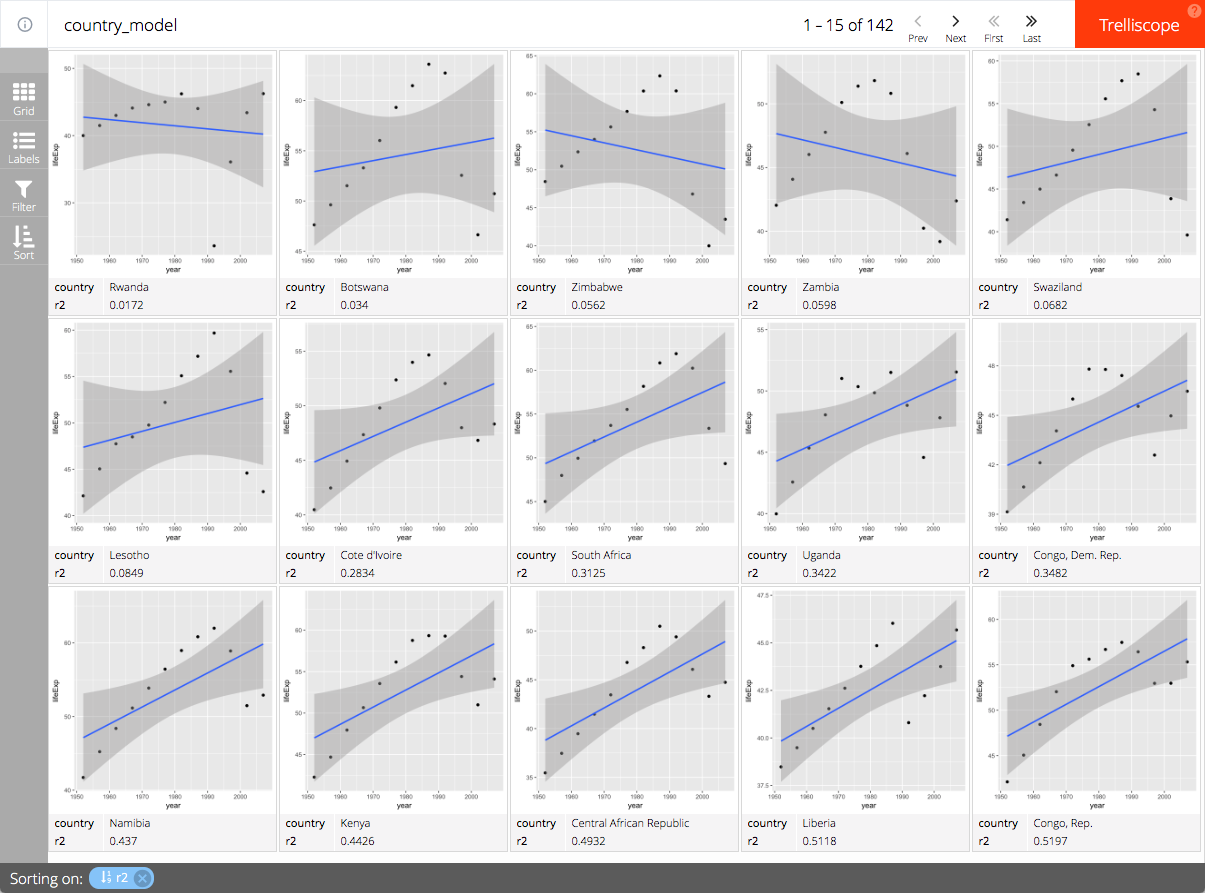
\includegraphics[height=4in]{./figs/tjs_country_r2.png}
  \caption{A \trelliscopejs~widget of country life expectancy over time where the panel ordering is displayed according to ascending $R^2$ value of each panels linear model.}
\end{figure}



In less than ten lines of code we went from a single data set to a full fledge visualization application with multiple cognostics explaining the plot used with each conditioned subset.


\section{Summary}

  Automatic cognostics with the \autocogs~R package allow users to enable common univariate metrics that correspond to the plots displayed in a \trelliscopejs~HTML widget. \autocogs~provides users with the ability to retrieve statistical metrics that are displayed or utilized in a plot.  Prior examples generated cognostics for simple histograms to multiple layered, linear model and scatterplot plots. Maintaining a common set of cognostics provides a cohesive cognostic framework to be used by any plotting architecture.



\chapter{GQLR: A GRAPHQL R SERVER IMPLEMENTATION} \label{chapter:gqlr}



% Extra cites
% https://en.wikipedia.org/wiki/Key-value_database
% https://en.wikipedia.org/wiki/Strong_and_weak_typing
% https://en.wikipedia.org/wiki/Hypertext_Transfer_Protocol
% https://en.wikipedia.org/wiki/Application_programming_interface


Since 2012, Facebook has developed GraphQL: ``a query language for APIs and a runtime"~\cite{graphql_org}.  GraphQL drastically reduces the number of server requests created by the browser by using a dynamic and nested query structure.  Using the Working Draft Specification for GraphQL~\cite{graphql_spec} as guidance, \gqlr~\cite{r_gqlr}~implements a full GraphQL server within R.  \gqlr~allows users to supply their own R functions to satisfy the data requirements of a GraphQL query generated by the browser.  \gqlr~was originally built to communicate between \trelliscopejs~and an R server session.  However, \trelliscopejs's development direction has changed since the creation of \gqlr.


\section{Application protocol interfaces}

Application Protocol Interfaces (APIs) are the fundamental backbone of communication between machines.  They enable machines to communicate with each other without needing to know how the responding machine arrives at its answer.  There are two conventions for a machine API: simple API and custom API.  Each API style has their own advantages and disadvantages.  GraphQL was created to address the disadvantages of simple API while keeping the advantages of a custom API at the cost of typing the request.


There are two parts involved in each API communication: the request and response.  The request submits a query to the server, and the response returns an answer that should be able to be understood by the requesting entity.  The key point to the communication transaction is the request does not need to know how the response calculates the answer.

This layer of abstraction shields the request from knowing the nitty-gritty implementation details of the response.  This allows the response to behave like a black box that will only respond to particular requests or queries.


In this chapter, I will only address single response APIs as I am concerned with the request, not the response.  A single response API is an API that returns only one response to one answer.  I will not discuss streaming APIs in this chapter.

Throughout this section, I will use a calculator, `Calculator', as my example server.  The calculator will be have four internal functions: add, subtract, multiply, and divide.  These four internal functions behave just like a regular calculator, but the true implementation of the calculator is hidden.

\subsection{Simple API}

% There are two common styles of single response APIs: simple and custom response.
A simple API has a single end point, or place to send a request, for each style of question it knows how to answer.  A simple Calculator API would contain four end points: add, subtract, multiply, and divide.  Each query routine requires two numeric values as inputs and responds with a single numeric value.  To concisely define a RESTful Calculator, we may state the following schema:

\begin{graphqlcode}
# GraphQL; Schema
type Calculator {
  add(A: Float, B: Float): Float
  subtract(A: Float, B: Float): Float
  multiply(A: Float, B: Float): Float
  divide(A: Float, B: Float): Float
}
\end{graphqlcode}

\subsubsection{Advantages}

Without abstracting the function name, the number of request end points match the number of exposed functions.  There are no dynamically created functions; everything is static.  By fixing all request end points, software systems can be reliably built against one another.  Any software system can build their own logic as to how they solve their particular problems, but each software system will request from the same API.

The ease of use of a simple API has made it very popular with HTTP internet websites with the RESTful API~\cite{rest_popular}.  The four most common functions of HTTP's REST are ``GET'', ``PUT'', ``POST'', and ``DELETE''.

\begin{enumerate}
  \item GET: Retrieve the supplied location data only.
  \item PUT: Store supplied data the supplied location.
  \item POST: Add new data at the supplied location.
  \item DELETE: Remove data at the supplied location.
\end{enumerate}


\subsubsection{Disadvantages}

As is common in practice, databases have many tables with built in relationships. RESTful APIs usually only return information one layer deep.

When looking at the Calculator, it solves a single calculation for each query.  To solve a multiple calculation problem, it takes multiple requests to the Calculator API.  For example, solving $1 + 2 + 3 + 4 + 5$ requires 4 requests to the Calculator API; one query for each of the $addition$ operations.

\begin{knitrout}\small
\definecolor{shadecolor}{rgb}{0.969, 0.969, 0.969}\color{fgcolor}\begin{kframe}
\begin{alltt}
\hlstd{answer} \hlkwb{=} \hlstd{Calculator}\hlopt{::}\hlkwd{add}\hlstd{(}\hlnum{1}\hlstd{,} \hlnum{2}\hlstd{)} \hlcom{# 3}
\hlstd{answer} \hlkwb{=} \hlstd{Calculator}\hlopt{::}\hlkwd{add}\hlstd{(answer,} \hlnum{3}\hlstd{)} \hlcom{# 6}
\hlstd{answer} \hlkwb{=} \hlstd{Calculator}\hlopt{::}\hlkwd{add}\hlstd{(answer,} \hlnum{4}\hlstd{)} \hlcom{# 10}
\hlstd{answer} \hlkwb{=} \hlstd{Calculator}\hlopt{::}\hlkwd{add}\hlstd{(answer,} \hlnum{5}\hlstd{)} \hlcom{# 15}
\end{alltt}
\end{kframe}
\end{knitrout}

No matter how the requests are altered, it will require 4 requests to the Calculator.  This can become a major disadvantage when required to make many, many requests to the API.  If we were to look at a person's friends of their friends, we would need the following Schema and data information:

\begin{graphqlcode}
# GraphQL; Schema
type Person {
  id: ID
  name: String
  age: Int
  sex: String
  friends: [ID]
}
\end{graphqlcode}

Each person has an ``id'', ``name'', ``age'', ``sex'', and a list of person id's for their ``friends''.  While having all of this information is useful, it can bloat the amount of information that is returned.  While the current example isn't too big, one could imagine adding a \graphqlinline{Person}'s favorite song lyrics to the \graphqlinline{Person} object.  This would greatly increase the total amount of information returned for each \graphqlinline{Person} object.

\subsection{REST and the Internet}

In the case of the internet, however, two major constraints exist.  The two major constraints are the number of parallel requests that can be made at one time and the amount of time it takes for your request to reach a responding server.

HTTP 1.1 specification states that ``A single-user client SHOULD NOT maintain more than 2 connections with any server or proxy''~\cite{http_connections}.  In practice, this is a little larger, maxing out at 13 parallel connections to the same host~\cite{browserscope}.  Limiting the number of server connections reduces the amount of simultaneous requests on the network and improves overall response time.

Once a request is allowed to be made, there are physical limitations on how fast the response can be received.  On average, it takes over 200 ms for a request to make a trip to the responding server and back to the user's browser~\cite{internetweathermap}.

Using the ``friends of my friends'' example, let us define each person as having 200 different friends (the median number of friends on Facebook~\cite{facebook_friends}.  When using a simple API, we can calculate how many requests are necessary to compute who are the ``friends of my friends''. It requires $O(n^2) (\sim 200^2 = 40,000)$ independent requests to the simple API server.  If the browser being used is limited to 10 parallel connections, it requires $4000 (= 40,000 / 10)$ sets of parallel request groups.  Each parallel request group takes at least 200ms for a round trip to and from the server.  The total amount of time it would require to gather the names of a person's friends of friends is approximately $13 \frac{1}{3} minutes = \dfrac{(200 requests)^2}{10 requests} * \dfrac{0.200 \frac{seconds}{request}}{60 \frac{seconds}{minute}}$.

The median loading time for a website is about 3 seconds with the average around 5 seconds~\cite{website_speed}.  Major websites today try to shave milliseconds where ever they can.  No major website would allow a load time that is 160 times slower than the average website.

% With the average website is now requiring more than 100 requests per page (http://www.websiteoptimization.com/speed/tweak/average-number-web-objects/), website turn around is decreasing.


\subsection{Custom response}

A natural response to the ``friends of my friends'' situation is implement a custom response which directly answers the specific query.

\subsubsection{Advantages}

Because custom APIs answer specific questions, only one request needs to be sent to the server.  The ``friends of my friends'' example is reduced to a single, 200 ms request.  The load time is now reduced from 800 seconds to 0.2 seconds.  This answers the ``who are my friends of my friends'' question in the minimal amount of queries to the server.  The custom API achieves the end goal answer with the minimal amount of queries ($1$) to the server.

\subsubsection{Disadvantages}

The disadvantages come from the amount of engineering time that is required to implement a custom response for every query need.  With a simple query interface, the logic is put on the user who is querying to figure out what to query next.  With a custom response interface, all custom responses must be made before the user can utilize them.

Using the Calculator example, calculating the $1 + 2 + 3 + 4 + 5$ example could be done in a single custom request called ``1add2add3add4add5''.  It would solve the answer in a single request, but the server would have to implement many, many responses for full funtionality of a true Calculator.

With the internet, the custom API response is now tied directly to the requesting website.  This creates little separation between the website and the responding API server.  By coupling the data server with the requesting service, developments in the requests are slower and more difficult than if a de-coupled, simple API is used.  Websites making the requests can not move ahead in development until a new custom response has been enabled by the custom API server.

\subsection{Balancing act}

Let's recap the advantages and disadvantages of the two different styles of APIs.

\begin{enumerate}
  \item Simple API
    \begin{enumerate}
      \item Advantages
        \begin{enumerate}
          \item Small API
          \item Easier to implement
        \end{enumerate}
      \item Disadvantages
      \begin{enumerate}
        \item Many queries are required to solve complex problems
        \item Many queries causes large time complexity
        \item Every piece of information is returned for every query
      \end{enumerate}
    \end{enumerate}
  \item Custom Responses
    \begin{enumerate}
      \item Advantages
        \begin{enumerate}
          \item One query, one answer
          \item Fast execution time
        \end{enumerate}
      \item Disadvantages
        \begin{enumerate}
          \item All custom API calls need to be implemented
          \item API server is tied to the requests made
        \end{enumerate}
    \end{enumerate}
\end{enumerate}

% It is a balancing act to use a simple API, which causes more requests, and a

Developers balance between minimal engineering time and minimal execution time.  Typically the final result falls somewhere in-between, using a custom API for high execution time queries and using a simple API for smaller queries.



% \section{Variable typing}
%
% Programming languages know the type of objects in two ways: strong typed and weakly typed.  Strong typed languages know ``whenever an object is passed from a calling function to a called function, its type must be compatible with the type declared in the called function.''~\cite{Liskov74programmingwith}.  Weakly typed languages allow a programmer to passively use a invalid type as if it was correct.  Using Javascript, we can define a function that returns the square of an object's key $key$. The function does not define any requirements about the variable $x$.  The \emph{hope} is that the function will only be called with a valid object type.
%  %~\cite{crockford2008javascript}.
%
% \begin{jscode}
% // javascript
% square_key = function(x) {
%   return x.key * x.key;
% }
% square_key({key: 5})
% // 25
% square_key(5)
% // NaN
% \end{jscode}
%
% In a strong typed C++ example, an integer is not cast into a \cppinline{KeyVal} object. By requiring variable types for inputs and outputs, the variable class is known at compile time and the program may be checked for type errors.
%
% \begin{cppcode}
% // C++
% struct KeyVal {
%   double key;
% };
% double square_key(KeyVal x) {
%   return x.key * x.key;
% };
% int main() {
%   KeyVal x;
%   x.key = 5;
%   std::cout << square_key(x); // Would print "25"
%   std::cout << square_key(5); // Causes compile error
% }
% // In function 'int main()':
% // 12:26: error: could not convert '5' from 'int' to 'KeyVal'
% \end{cppcode}

\section{Database storage}

Once a request is received by an API, the API must retrieve the data from a database.  Databases can store objects in one of two common paradigms: as a relational database or as a key-value database.  Relational databases know exactly what kind of object will be returned and can map one table to another with id values.  Key-value databases, on the other hand, do not inspect the values of the database.  The requirement for a key-value database is that each value is stored at a specific key.  Key-value databases are built for speed and scalability over structure and relationships.

While relational databases are already inherently typed (unless purposely stated as an unknown type), well designed key-value databases inherently contain typed values.  Each value that is inserted into the database has a known shape and expected response type.  If data of an image is stored, audio data should never be returned from that same position.  Even if the image had different sizes and formats, it still can be understood as an image.

There are many more comparisons and cost / benefits to every database, however these implementation differences are not apart of the scope of this chapter.



\section{GraphQL language}

GraphQL is a data query language built to unify data APIs.  It exists as a execution layer between the requesting user and responding database.  This abstraction layer provides many benefits: uniform request and response shape, dynamic queries to handle custom situations, and minimal server requests.

GraphQL is comprised of two main parts, the Request and the Schema.

\subsection{Schema}

GraphQL Schemas are defined using Scalars, Types, Enumerations, Lists, Non-Null types, Interfaces, Unions, and Input types.  Each definition is used to define a type or type abstractions that can be used when querying.  The Types represent the expected return objects that the database already knows about from the Schema definition.  Like most objects, each Object Type will contain fields that point to Scalars or more Types.  These Object fields can be queried recursively until a Scalar or Enumeration is reached.

\subsubsection{Object type definition}

For example, we can setup a Schema for a pet dog.

\begin{graphqlcode}
type Dog {
  name: String
  breed: String!
  owners: [Person!]!
}
\end{graphqlcode}

The type definition for a \graphqlinline{Dog} is very readable, but has a lot going on.

\begin{enumerate}
  \item \graphqlinline{Dog} is a Object Type definition.  It has four fields:  \graphqlinline{name}, \graphqlinline{breed}, \graphqlinline{age}, and \graphqlinline{owners}.  These four fields are the only fields defined for retrieving information from a \graphqlinline{Dog}.
  \item \graphqlinline{String} is a predefined Scalar type definition.  This contains the dog's name, i.e. ``Clifford''.  Scalar fields do not contain any sub fields and are considered leafs in the Schema definition tree. Leafs do not contain sub fields for further information retrieval.
  \item \graphqlinline{String!} represents a Non-null String value.  This means that all \graphqlinline{Dog} objects will contain the \graphqlinline{breed} field and the result will always be a String.
  \item \graphqlinline{[Person]} represents an array of Person objects that represent the owners of the Dog. By adding the \graphqlinline{!} outside the array to form \graphqlinline{[Person]!}, it will be guaranteed to return an array for the field \graphqlinline{owners} and never a \graphqlinline{NULL} value.  By adding a \graphqlinline{!} to the Person (\graphqlinline{[ Person!]!}), the elements inside the position array will never be \graphqlinline{NULL}.  A length $0$ array is still allowed as the \graphqlinline{owners} value is not \graphqlinline{NULL} and the missing \graphqlinline{Person} values are not \graphqlinline{NULL}.
\end{enumerate}


\subsection{Argument and input type definitions}

Field definitions can include arguments.  These arguments can be simple Scalar definitions or Input Type definitions.

\begin{graphqlcode}
# GraphQL; Schema
input ToyInput {
  brand: String
  name: String
  condition: Condition
}
extend type Dog {
  weight(unit: WeightUnit = POUNDS): Float
  does_play_with_toy(toy: ToyInput): Boolean
}
\end{graphqlcode}

Like the R language, all arguments are named arguments, all arguments may be submitted in any order, and default values may be provided.  Unlike R, all submitted arguments must have a name and must comply with the argument type.  Nothing is inferred from the arugment's position.  Default values may be used in place of missing arguments.

\subsection{Schema type definition}

There are two entry points to a Schema: schema query type and schema mutation type. Every GraphQL Schema definition must have a schema query type and can optionally have a schema mutation type.  Both types refer to an object type definition.

\begin{graphqlcode}
# GraphQL; Schema
schema {
  query: Dog
  mutation: DogUpdate
}
\end{graphqlcode}

Query types are read only, while mutation types are understood that something will update in the database.  A request will have the same shape for both query types and mutation types.

\subsection{Scalar type definitions}

Scalar Types are the leafs of the Schema.  Unlike Object Types, Scalars do not have fields to inspect.  GraphQL defines the base scalars as a part of the language definition:

\begin{enumerate}
  \item \graphqlinline{Boolean}: $true$ or $false$
  \item \graphqlinline{Integer}: A signed 32-bit integer
  \item \graphqlinline{Float}: A signed double-precision floating point value
  \item \graphqlinline{String}: A UTF-8 character sequence
  \item \graphqlinline{ID}: \graphqlinline{ID} performs the same as a \graphqlinline{String}, but it is intended to be machine readable only as a unique identifier
\end{enumerate}

New scalars can be defined in a Schema as long as the server running the GraphQL understands how to handle them.  Three new Scalars are defined below.

\begin{graphqlcode}
# GraphQL; Schema
scalar Date
scalar Binary
scalar Hexadecimal
\end{graphqlcode}



\subsection{Enumeration type definitions}

GraphQL understands a finite category variable.  This is similar to a \rinline{factor} in R.  There is a fixed set of values for every Enum definition.  Internally in the GraphQL server, Enum definitions may be stored as Integer values or as an object similar to a Set, but in the GraphQL language, it will be represented as a string with all capitol letters, such as \graphqlinline{POUNDS}.

\begin{graphqlcode}
# GraphQL; Schema
enum WeightUnit {
  POUNDS
  KILOS
  OUNCES
}
\end{graphqlcode}

Whenever a \graphqlinline{WeightUnit} type is expected, only the values of \graphqlinline{POUNDS}, \graphqlinline{KILOS}, or \graphqlinline{OUNCES} may be used.  While R supports \rinline{factor} values, and full Enumeration class is created in the \gqlr~R package.


\subsection{Interface type definition}

Interfaces are an integral part in abstracting pieces of types of objects.  They allow for common fields to be accessed on objects without knowing the true type of the object.  All Object Types that inherit an interface must implement all fields of that interface.  Any Object Type that implements \graphqlinline{Pet}, must implement the two fields \graphqlinline{name} and \graphqlinline{owners} and return \graphqlinline{String} and \graphqlinline{[Person!]!} respectively.

\begin{graphqlcode}
# GraphQL; Schema
interface Pet {
  name: String
  owners: [Person!]!
}
type Dog implements Pet {
  name: String
  barkVolume: Int
  owners: [Person!]!
}
type Cat implements Pet {
  name: String
  meowVolume: Int
  owners: [Person!]!
}
\end{graphqlcode}

An Object Type may implement extra fields, like \graphqlinline{meowVolume} in \graphqlinline{Cat}.

Interfaces are useful when queries are made on objects where the exact return type is not known, but a finite set of types exist for the expected value.

\begin{graphqlcode}
# GraphQL; Schema
extend type Person {
  pet: [Pet!]! # returns an array of Cat or Dog types
}
\end{graphqlcode}

Object definitions may interface with many Interface definitions.

\subsection{Union type definition}

Unions contain a finite set of Object Types but do not specify common fields.  Unions are not allowed to contain other unions or interfaces.  \graphqlinline{NotAPlant} results being returned could either be a \graphqlinline{Person}, \graphqlinline{Dog}, or \graphqlinline{Cat} type.

\begin{graphqlcode}
# GraphQL; Schema
extend type Cat {
  weight(unit: WeightUnit = KILOS): Float
}
union NotAPlant = Person | Dog | Cat
\end{graphqlcode}


\section{Requests}

The following Schema will be used within the Requests section.  Classic Disney characters will be used as the data.

\begin{graphqlcode}
# GraphQL; Schema
scalar Date
enum WeightUnit {
  POUNDS
  KILOS
  OUNCES
}
type Person {
  name: String!
  weight(unit: WeightUnit = POUNDS): Float
  friends: [Person!]!
  pets: [Pet!]!
}
\end{graphqlcode}
\begin{graphqlcode}
interface Pet {
  name: String
  born: Date
  owners: [Person!]!
}
type Dog implements Pet {
  name: String
  barkVolume: String
  born: Date
  owners: [Person!]!
}
type Cat implements Pet {
  name: String
  born: Date
  meowVolume: String
  owners: [Person!]!
}
union SearchResult = Person | Dog | Cat
\end{graphqlcode}
\begin{graphqlcode}
type QueryType {
  search_name(name: String!): SearchResult
  person(name: String! = "Mickey Mouse"): Person
  dog(name: String! = "Pluto"): Dog
  cat(name: String! = "Figaro"): Cat
}
type MutationType {
  addToWealth(name: String!, amount: Float): Float
}
schema {
  query: QueryType
  mutation: MutationType
}
\end{graphqlcode}


\subsection{Queries}

Every object in the Schema definition can be queried.  A query on an object type must include at least one field.  Object Types are not considered leafs in the Schema definition tree as they are guaranteed to have at least one field.

\begin{graphqlcode}
# GraphQL; Query
{
  person {
    name
  }
}
\end{graphqlcode}
\begin{jscode}
// JSON; GraphQL Response
{
  "data":{
    "person": {
      "name": "Mickey Mouse"
    }}}
\end{jscode}

Queries have the same shape has the result.  The only difference occurs when a result is an array of information.  Using an \graphqlinline{name} argument below, we can look at Jim Dear's pets from the movie ``Lady and the Tramp''~\cite{jimdear}.

\begin{graphqlcode}
# GraphQL; Query
{
  person(name: "Jim Dear") {
    name
    pets {
      name
    }}}
\end{graphqlcode}
\begin{jscode}
// JSON; GraphQL Response
{
  "data":{
    "person": {
      "name": "Jim Dear",
      "pets": [
        { "name": "Lady" },
        { "name": "Tramp" }
      ]}}}
\end{jscode}


The whole query string is submitted to the GraphQL server.  This allows for complex and deeply nested queries in a single request.  Using the query below, we can query for all pets owned by the same owners as Duchess the cat~\cite{madame}.

\begin{graphqlcode}
# GraphQL; Query
{
  cat(name: "Duchess") {
    owners {
      name
      pets {
        name
      }}}}
\end{graphqlcode}
\begin{jscode}
// JSON; GraphQL Response
{
  "data": {
    "cat": {
      "owners": [{
        "name": "Madame Adelaide Bonfamille",
        "pets": [
          {"name": "Duchess"},
          {"name": "Marie"},
          {"name": "Berlioz"},
          {"name": "Toulouse"},
          {"name": "Thomas O'Malley"}
        ]}]}}}
\end{jscode}

Normally the code above would require $O(k * n)$ requests in a simple API, with $k$ owners and $n$ pets belonging to each owner.  With GraphQL, this query is resolved in one request and without the need for a custom API to be built.  The single GraphQL query needed for the ``friends of my friends'' example is shown below.

\begin{graphqlcode}
# GraphQL; Query
{
  person(name: "Barret") {
    friends {
      name
      friends {
        name
      }}}}
\end{graphqlcode}






\subsubsection{Aliases}

Aliases can be used to query the same object field multiple times.


\begin{graphqlcode}
# GraphQL; Query
{
  duchess: cat(name: "Duchess") {
    name
    meowVolume
  }
  rajah: cat(name: "Rajah") {
    name
    meowVolume
  }}
\end{graphqlcode}

\begin{jscode}
// JSON; GraphQL Response
{
  "data": {
    "duchess": {
      "name": "Duchess",
      "meowVolume": 2
    },
    "rajah": {
      "name": "Rajah",
      "meowVolume": 9
    }}}
\end{jscode}

% \end{tabular}


\subsubsection{Fragments}

For conciseness, the multiple cat query can be made using Fragments.  Fragments can be used when repeated fields are called on similar objects.

The same result will occur using the Fragments below.

\begin{graphqlcode}
# GraphQL; Query
{
  duchess: cat(name: "Duchess") {
    ...catFields
  }
  rajah: cat(name: "Rajah") {
    ...catFields
  }
}
fragment catFields on Cat {
  name
  meowVolume
}
\end{graphqlcode}
\begin{jscode}
// JSON; GraphQL Response
{
  "data": {
    "duchess": {
      "name": "Duchess",
      "meowVolume": 2
    },
    "rajah": {
      "name": "Rajah",
      "meowVolume": 9
    }}}
\end{jscode}

Fragments are very useful in breaking down complex queries into smaller sections.

\subsection{Mutation}

Mutations are the ``write'' to a database.  Mutations also return information to avoid an immediate ``read'' afterwards.  While there is no guarentee that a Query does not alter the database, it is a good practice to distinguish which commands read only and which commands write to the database. The mutation example below adds to the wealth of Scrooge McDuck~\cite{scrooge}.

\begin{graphqlcode}
# GraphQL; Schema
type MutationType {
  # returns total wealth after adding amount
  addToWealth(name: String!, amount: Float): Float
}
\end{graphqlcode}
\begin{graphqlcode}
# GraphQL; Mutation
mutation {
  addToWealth(name = "Scrooge", amount = 1000.0)
}
\end{graphqlcode}
\begin{jscode}
// JSON; GraphQL Response
{
  "data": {
    "addToWealth": 28800000
  }}
\end{jscode}


\subsection{Remaining GraphQL language}

There are many more intricacies in the GraphQL language that are not in the scope of this paper.



\section{\gqlr: A GraphQL R server implementation}

\gqlr~is an R package that implements the GraphQL server specification.  \gqlr~handles Query and Mutation Requests and returns data in the proper format.  It is built upon the next evolution of class definitions in R, \pkg{R6}~\cite{r_r6}.

\subsection{\pkg{R6}}

\pkg{R6}~is a lightweight R package that creates objects that do not follow the particular conventions of R.  R known for being ``pass by value'' language. This means that all values are copied at the beginning of a function. Like many other languages, R does not have dynamic values for a list object.  Values placed in a list in R stay as the same values.

\begin{knitrout}\small
\definecolor{shadecolor}{rgb}{0.969, 0.969, 0.969}\color{fgcolor}\begin{kframe}
\begin{alltt}
\hlstd{my_list} \hlkwb{<-} \hlkwd{list}\hlstd{(}\hlkwc{A} \hlstd{=} \hlnum{TRUE}\hlstd{,} \hlkwc{B} \hlstd{=} \hlnum{FALSE}\hlstd{)}
\hlstd{my_list}\hlopt{$}\hlstd{A}
\end{alltt}
\begin{verbatim}
## [1] TRUE
\end{verbatim}
\begin{alltt}
\hlstd{update_A_to_false} \hlkwb{<-} \hlkwa{function}\hlstd{(}\hlkwc{x}\hlstd{) \{}
  \hlstd{x}\hlopt{$}\hlstd{A} \hlkwb{<-} \hlnum{FALSE}
  \hlstd{x}
\hlstd{\}}
\hlkwd{update_A_to_false}\hlstd{(my_list)}
\end{alltt}
\begin{verbatim}
## $A
## [1] FALSE
## 
## $B
## [1] FALSE
\end{verbatim}
\begin{alltt}
\hlstd{my_list}
\end{alltt}
\begin{verbatim}
## $A
## [1] TRUE
## 
## $B
## [1] FALSE
\end{verbatim}
\end{kframe}
\end{knitrout}

This R example does not update the value of A to \rinline{FALSE} as the value \rinline{my_list} was copied at the beginning of the function \rinline{update_A_to_false}.

\pkg{R6}~allows for objects to be altered inside functions that they have been passed to without any changes in assignment method.  This is similar to a ``pass by reference'' coding paradigm.  An \pkg{R6}~object is passed to a function and the function alters the value.  The same \pkg{R6}~object outside of the function is altered as well.  This is not expected R behavior.

\pkg{R6}~is built upon the use of Classes.  \pkg{R6}~classes are similar to Javascript's ES6 classes.  There is a constructor, methods, and values for each class.  The methods and values can be both private (only able to be seen internally) and public (available to anything).  Like Javascript, there is a notion of the ``this'' value or an object representing itself.  \pkg{R6}~uses the \rinline{self} object in this case.  Internal object values are retrieved using \rinline{value <- self\$key}.  The example below defines a new object \rinline{barret} with the name of \rinline{"Barret"}.  Unlike regular R behavior, the name is changed globally to \rinline{"Schloerke"} by calling the function \rinline{update_name_to_schloerke}.



\begin{knitrout}\small
\definecolor{shadecolor}{rgb}{0.969, 0.969, 0.969}\color{fgcolor}\begin{kframe}
\begin{alltt}
\hlstd{Minimal} \hlkwb{<-} \hlkwd{R6Class}\hlstd{(}\hlstr{"Minimal"}\hlstd{,}
  \hlkwc{public} \hlstd{=} \hlkwd{list}\hlstd{(}
    \hlkwc{name} \hlstd{=} \hlkwa{NULL}\hlstd{,}
    \hlkwc{initialize} \hlstd{=} \hlkwa{function}\hlstd{(}\hlkwc{name} \hlstd{=} \hlnum{NA}\hlstd{) \{}
      \hlstd{self}\hlopt{$}\hlstd{name} \hlkwb{<-} \hlstd{name}
      \hlstd{self}\hlopt{$}\hlkwd{greet}\hlstd{()}
    \hlstd{\},}
    \hlkwc{greet} \hlstd{=} \hlkwa{function}\hlstd{() \{}
      \hlkwd{cat}\hlstd{(}\hlkwd{paste0}\hlstd{(}\hlstr{"Hello, my name is "}\hlstd{, self}\hlopt{$}\hlstd{name,} \hlstr{".\textbackslash{}n"}\hlstd{))}
    \hlstd{\}}
  \hlstd{)}
\hlstd{)}
\hlstd{barret} \hlkwb{<-} \hlstd{Minimal}\hlopt{$}\hlkwd{new}\hlstd{(}\hlstr{"Barret"}\hlstd{)}
\end{alltt}
\begin{verbatim}
## Hello, my name is Barret.
\end{verbatim}
\begin{alltt}
\hlstd{barret}\hlopt{$}\hlstd{name}
\end{alltt}
\begin{verbatim}
## [1] "Barret"
\end{verbatim}
\begin{alltt}
\hlstd{update_name_to_schloerke} \hlkwb{<-} \hlkwa{function}\hlstd{(}\hlkwc{x}\hlstd{) \{}
  \hlstd{x}\hlopt{$}\hlstd{name} \hlkwb{<-} \hlstr{"Schloerke"}
  \hlkwd{invisible}\hlstd{(x)}
\hlstd{\}}
\hlkwd{update_name_to_schloerke}\hlstd{(barret)}
\hlstd{barret}\hlopt{$}\hlstd{name}
\end{alltt}
\begin{verbatim}
## [1] "Schloerke"
\end{verbatim}
\end{kframe}
\end{knitrout}


\pkg{R6}~also allows for dynamic queries.  \pkg{R6}~calls these ``active fields''.  These fields are actually function calls, but appear a regular keys in the object.  The active key function can handle a single argument.  This argument represents the value of the object being stored.  If no value was supplied, then the active key was retrieved, not set.

In the example below, a single active key of $random$ will return a uniform value when retrieved and will set the random seed if the $random$ key is set.  After the key is set to $1234$, as expected, the same random values are returned.

\begin{knitrout}\small
\definecolor{shadecolor}{rgb}{0.969, 0.969, 0.969}\color{fgcolor}\begin{kframe}
\begin{alltt}
\hlstd{MinimalActive} \hlkwb{<-} \hlkwd{R6Class}\hlstd{(}\hlstr{"MinimalActive"}\hlstd{,}
  \hlkwc{active} \hlstd{=} \hlkwd{list}\hlstd{(}
    \hlkwc{random} \hlstd{=} \hlkwa{function}\hlstd{(}\hlkwc{x}\hlstd{) \{}
      \hlkwa{if} \hlstd{(}\hlkwd{missing}\hlstd{(x)) \{}
        \hlkwd{return}\hlstd{(}\hlkwd{runif}\hlstd{(}\hlnum{1}\hlstd{))}
      \hlstd{\}}
      \hlkwd{set.seed}\hlstd{(x)}
      \hlnum{TRUE}
    \hlstd{\}}
  \hlstd{)}
\hlstd{)}
\hlstd{min_active} \hlkwb{<-} \hlstd{MinimalActive}\hlopt{$}\hlkwd{new}\hlstd{()}
\hlstd{min_active}\hlopt{$}\hlstd{random}
\end{alltt}
\begin{verbatim}
## [1] 0.9829186
\end{verbatim}
\begin{alltt}
\hlstd{min_active}\hlopt{$}\hlstd{random}
\end{alltt}
\begin{verbatim}
## [1] 0.5822385
\end{verbatim}
\begin{alltt}
\hlstd{min_active}\hlopt{$}\hlstd{random} \hlkwb{<-} \hlnum{1234}
\hlstd{min_active}\hlopt{$}\hlstd{random}
\end{alltt}
\begin{verbatim}
## [1] 0.1137034
\end{verbatim}
\begin{alltt}
\hlstd{min_active}\hlopt{$}\hlstd{random}
\end{alltt}
\begin{verbatim}
## [1] 0.6222994
\end{verbatim}
\begin{alltt}
\hlstd{min_active}\hlopt{$}\hlstd{random} \hlkwb{<-} \hlnum{1234}
\hlstd{min_active}\hlopt{$}\hlstd{random} \hlcom{# same value as the first random value with seed 1234}
\end{alltt}
\begin{verbatim}
## [1] 0.1137034
\end{verbatim}
\end{kframe}
\end{knitrout}

Finally, \pkg{R6}~allows for inheritance.  In the GraphQL's abstract syntax tree, many objects inherit from one another in a directed, acyclic graph structure.  \pkg{R6}'s class inheritance extends nicely to the abstract syntax tree requirments of GraphQL.

\begin{knitrout}\small
\definecolor{shadecolor}{rgb}{0.969, 0.969, 0.969}\color{fgcolor}\begin{kframe}
\begin{alltt}
\hlstd{ParentClass} \hlkwb{<-} \hlkwd{R6Class}\hlstd{(}\hlstr{"ParentClass"}\hlstd{)}
\hlstd{ChildClass} \hlkwb{<-} \hlkwd{R6Class}\hlstd{(}\hlstr{"ChildClass"}\hlstd{,} \hlkwc{inherit} \hlstd{= ParentClass)}
\hlstd{child} \hlkwb{<-} \hlstd{ChildClass}\hlopt{$}\hlkwd{new}\hlstd{()}
\hlkwd{class}\hlstd{(child)}
\end{alltt}
\begin{verbatim}
## [1] "ChildClass"  "ParentClass" "R6"
\end{verbatim}
\begin{alltt}
\hlkwd{inherits}\hlstd{(child,} \hlstr{"ParentClass"}\hlstd{)}
\end{alltt}
\begin{verbatim}
## [1] TRUE
\end{verbatim}
\end{kframe}
\end{knitrout}

In \gqlr, all active values must inherit the correct class to be allowed to set.  An Error will be thrown if a value does not contain the proper inheritance.  The example below shows the creation of a named type ``Dog''.  It also shows an attempt at setting the $name$ value to a character.  This is not allowed as the $name$ value only allows objects that inherit the class ``Name''.

\begin{knitrout}\small
\definecolor{shadecolor}{rgb}{0.969, 0.969, 0.969}\color{fgcolor}\begin{kframe}
\begin{alltt}
\hlstd{(obj} \hlkwb{<-} \hlstd{gqlr}\hlopt{:::}\hlstd{NamedType}\hlopt{$}\hlkwd{new}\hlstd{(}\hlkwc{name} \hlstd{= gqlr}\hlopt{:::}\hlstd{Name}\hlopt{$}\hlkwd{new}\hlstd{(}\hlkwc{value} \hlstd{=} \hlstr{"Dog"}\hlstd{)))}
\end{alltt}
\begin{verbatim}
## <graphql definition>
##   | Dog
\end{verbatim}
\begin{alltt}
\hlkwd{str}\hlstd{(obj}\hlopt{$}\hlstd{name)}
\end{alltt}
\begin{verbatim}
## <Name>
## . value: 'Dog'
\end{verbatim}
\begin{alltt}
\hlstd{obj}\hlopt{$}\hlstd{name} \hlkwb{<-} \hlstr{"Dog"}
\end{alltt}


{\ttfamily\noindent\bfseries\color{errorcolor}{\#\# Error in bad\_inherits(): Attempting to set NamedType.name.\\\#\# Expected value with class of |Name|.\\\#\# Received character}}\end{kframe}
\end{knitrout}

\gqlr~uses these active fields to accomplish typed language properties while executing in a untyped language of R.  While enforcing typing within R does not happen often, it is required for GraphQL to be implemented.

\subsection{Execution}

At first glance, R and GraphQL seem like an unlikely combination.  R is an untyped (dynamically typed) language while GraphQL is a typed language.  R is not known for its raw speed and one of GraphQL's goals is to reduce execution time.

However, R is known for its statistical models, statistical graphics, and its very fast iteration speed~\cite{r_about}.  \gqlr~is built to help small projects provide proof of concepts and for developers to mock full backend systems locally.  Being able to submit the same style of request string for the production server and local development increases the productivity of the web development cycle.

The example below creates a model schema that creates a linear model and a loess model.  Both models return the mean squared error (\rinline{mse}) for their respective models.  The linear model also returns a \GGally's \rinline{ggnostic} plot which is base64 encoded~\cite{josefsson2006base16} for data portability.  The loess model also returns the effective number of parameters (\rinline{enp}).

\begin{knitrout}\small
\definecolor{shadecolor}{rgb}{0.969, 0.969, 0.969}\color{fgcolor}\begin{kframe}
\begin{alltt}
\hlstr{"# GraphQL; Schema
scalar ImageBase64
type LinearModel \{ mse: Float!, ggnostic: ImageBase64! \}
type LoessModel \{ mse: Float!, enp: Float! \}
type Model \{
  linear(formula: String, data_name: String): LinearModel
  loess(formula: String, data_name: String): LoessModel
\}
schema \{ query: Model \}
"} \hlopt
  \hlstd{gqlr}\hlopt{::}\hlkwd{gqlr_schema}\hlstd{(}
    \hlkwc{ImageBase64} \hlstd{=} \hlkwa{function}\hlstd{(}\hlkwc{p}\hlstd{,} \hlkwc{schema}\hlstd{) \{}
      \hlstd{tmp_file} \hlkwb{<-} \hlkwd{tempfile}\hlstd{(}\hlkwc{fileext} \hlstd{=} \hlstr{".png"}\hlstd{)}
      \hlkwd{on.exit}\hlstd{(}\hlkwd{unlink}\hlstd{(tmp_file))}
      \hlstd{ggplot2}\hlopt{::}\hlkwd{ggsave}\hlstd{(tmp_file, p)}
      \hlstd{knitr}\hlopt{::}\hlkwd{image_uri}\hlstd{(tmp_file)} \hlopt
        \hlcom{# shorten for display purposes}
        \hlkwd{substr}\hlstd{(}\hlkwc{start} \hlstd{=} \hlnum{1}\hlstd{,} \hlkwc{stop} \hlstd{=} \hlnum{40}\hlstd{)} \hlopt
        \hlkwd{paste0}\hlstd{(}\hlstr{"..."}\hlstd{)}
    \hlstd{\},}
    \hlkwc{LinearModel} \hlstd{=} \hlkwa{function}\hlstd{(}\hlkwc{model}\hlstd{,} \hlkwc{schema}\hlstd{) \{}
      \hlkwd{list}\hlstd{(}
        \hlkwc{mse} \hlstd{=} \hlkwd{mean}\hlstd{(model}\hlopt{$}\hlstd{residuals} \hlopt{^} \hlnum{2}\hlstd{),}
        \hlkwc{ggnostic} \hlstd{=} \hlkwa{function}\hlstd{(}\hlkwc{...}\hlstd{) \{}
          \hlstd{GGally}\hlopt{::}\hlkwd{ggnostic}\hlstd{(model)}
        \hlstd{\})\},}
    \hlkwc{LoessModel} \hlstd{=} \hlkwa{function}\hlstd{(}\hlkwc{model}\hlstd{,} \hlkwc{schema}\hlstd{) \{}
      \hlkwd{list}\hlstd{(}
        \hlkwc{mse} \hlstd{=} \hlkwd{mean}\hlstd{(model}\hlopt{$}\hlstd{residuals} \hlopt{^} \hlnum{2}\hlstd{),}
        \hlkwc{enp} \hlstd{= model}\hlopt{$}\hlstd{enp}
      \hlstd{)\},}
    \hlkwc{Model} \hlstd{=} \hlkwa{function}\hlstd{(}\hlkwc{ignore}\hlstd{,} \hlkwc{schema}\hlstd{) \{}
      \hlstd{model_} \hlkwb{<-} \hlkwa{function}\hlstd{(}\hlkwc{fn_}\hlstd{) \{}
        \hlkwa{function}\hlstd{(}\hlkwc{null}\hlstd{,} \hlkwc{args}\hlstd{,} \hlkwc{schema}\hlstd{) \{}
          \hlstd{formula_} \hlkwb{<-} \hlkwd{as.formula}\hlstd{(args}\hlopt{$}\hlstd{formula)}
          \hlstd{data_} \hlkwb{<-} \hlkwd{eval}\hlstd{(}\hlkwd{as.symbol}\hlstd{(args}\hlopt{$}\hlstd{data_name))}
          \hlkwd{fn_}\hlstd{(formula_,} \hlkwc{data} \hlstd{= data_)}
        \hlstd{\}\}}
      \hlkwd{list}\hlstd{(}
        \hlkwc{linear} \hlstd{=} \hlkwd{model_}\hlstd{(stats}\hlopt{::}\hlstd{lm),}
        \hlkwc{loess} \hlstd{=} \hlkwd{model_}\hlstd{(stats}\hlopt{::}\hlstd{loess)}
      \hlstd{)\})} \hlkwb{->}
\hlstd{model_schema}
\end{alltt}
\end{kframe}
\end{knitrout}

In about 40 lines of code, a schema definition and execution methods can be implemented.  To build a strong typed API and its corresponding implementation in less than 100 lines is not an easy task.  With \gqlr, we are able to do it in less than half the lines of code.

In the implementation, four major R packages are called.

\begin{enumerate}
  \item \pkg{stats}~is used for the linear model function and loess function.
  \item \GGally~is used to call its model diagnostic plot matrix, \rinline{ggnostic}.
  \item \ggplot~is used to save the plot objected created by \GGally.
  \item \pkg{knitr}~is used for its ability to data64 encode images saved by \ggplot.
\end{enumerate}

These packages are built upon many other R packages and displays the extensibility of a schema execution.

To see the Model schema in action, we can execute a request using the classic R data set ``iris''.

\begin{knitrout}\small
\definecolor{shadecolor}{rgb}{0.969, 0.969, 0.969}\color{fgcolor}\begin{kframe}
\begin{alltt}
\hlstr{'# GraphQL; Query
\{
  linear(
    formula: "Petal.Length ~ Petal.Width",
    data_name: "iris"
  ) \{
    mse,
    ggnostic
  \}
  loess(
    formula: "Petal.Length ~ Petal.Width",
    data_name: "iris"
  ) \{
    mse,
    enp
  \}
\}'} \hlopt
  \hlstd{gqlr}\hlopt{::}\hlkwd{execute_request}\hlstd{(}\hlkwc{schema} \hlstd{= model_schema)} \hlkwb{->}
\hlstd{result}
\end{alltt}
\end{kframe}
\end{knitrout}

\begin{knitrout}\small
\definecolor{shadecolor}{rgb}{0.969, 0.969, 0.969}\color{fgcolor}\begin{kframe}
\begin{alltt}
\hlstd{result}
\end{alltt}
\begin{verbatim}
## {
##   "data": {
##     "linear": {
##       "mse": 0.2256,
##       "ggnostic": "data:image/png;base64,iVBORw0KGgoAAAANSU..."
##     },
##     "loess": {
##       "mse": 0.1444,
##       "enp": 4.0584
##     }
##   }
## }
\end{verbatim}
\end{kframe}
\end{knitrout}

While R users might not find the query and output very compelling (as they can be done in a regular R session), it is good to remember that any web service with access to the R \rinline{Model} schema can execute a similar command and get an answer that is executed by R.  During the request execution, \emph{any} R package can be used.  Being able to open the flood gates to R's extensive package list is very powerful. This allows Javascript in the browser and Python programs to retrieve full R plots and R model outputs using the same GraphQL API.

This schema can also be executed in a local GraphQL server session or on a production GraphQL server.  Both the local and production servers have the same schema, so each service will return the same shapes.  Each querying programming language will have the same query string and receive the same shaped response.


\subsection{Web service}

A simple web server is included in \gqlr, but extending the web server to other url routes and authentication services are not included.  \gqlr~was built to handle GraphQL requests and leave the url routing and authentication to better suited packages.  While some may argue for a single, go-to R package, there are many existing URL request handlers and authenticators existing for R.




\section{Summary}

  \gqlr~leverages the GraphQL language to effectively and efficiently communicate custom defined queries to and from the server.  \gqlr~provides users the ability to rapidly iterate in a local R environment to mock large production-scale data backends.  Combining R's fast iteration speed with R's ability to connect to many different existing backend services saves developers time and effort while keeping the data API communication consistent.






% There is a unique API or interaction method to query every database.  When making a database call to a MySQL server, there is a known SQL syntax for interacting with the relational database.  When making a database call to a MongoDB server, there is a different, known syntax for interacting with the NoSQL database.  For every known database, there is a unique language created to interact with the data.  If a database needs to be updated to a different database or is even upgraded to a new version, the query syntax, more often than not, is broken.  This leads to continuous integration with the query syntax and the database and constant reprogramming of the query syntax for every update of the database syntax.  GraphQL addresses this issue.



%
%  summary.tex  2007-02-06  Mark Senn  http://www.ecn.purdue.edu/~mark
%

\chapter{SUMMARY} % ~ 2 pages in total

% ~ 1/2 page
%
% In this thesis we have shown that
%   decribed three packages that i have worked on. (paraphrase the intro)
%     intro - ``we will do that''; ``we have done that''
%
% we have demonstrated....
%   repeat what you've done already
%
% This is the summary chapter.
%   review each chapter ~ 1-2 paragraphs
%   Remind how they integrate with each other


% In this thesis we have shown that
%   decribed three packages that i have worked on. (paraphrase the intro)
%     intro - ``we will do that''; ``we have done that''

In this thesis, I have described
\begin{enumerate}[i)]
  \item \rinline{ggduo}, an R function that produces generalized plot matrices for two groups of variables,
  \item \autocogs, an R package that automatically generates cognostics for a set of plots, and
  \item \gqlr, an R package which implements the GraphQL data query application protocol interface.
\end{enumerate}

\rinline{ggduo} extended the application of the generalized pairs plot to a generalized plot matrix for two-grouped data.  This function has direct application to canonical correlation analysis and was extended by \rinline{ggnostic} to produce a generalized plot matrix for model diagnostics and \rinline{ggts} to produce a generalized plot matrix for time series data.  These \ggplot-style plot matrices are implemented using the \rinline{ggmatrix} plot object in \GGally.

\autocogs~implemented multiple standard cognostic groups to be automatically produced given the different plot layers of a \ggplot~visualization. Each layer within a plot is connected to multiple cognostic groups.  These sets of cognostics are then leveraged within a \trelliscopejs~HTML widget to aid in its data panel exploration.  These cognostics alleviate the user from creating each cognostic value manually in the data set speeding up the data exploration process.

\gqlr~implemented the GraphQL server within the R environment.  The GraphQL query language minimized the number of incoming data requests.  By decoupling the websites and the stored data, iteration speed is increased in both web site development and data storage development.  \gqlr~enabled R users to make use of the GraphQL query language for efficient data extraction and statistical modeling.

\section{Discussion and Future Work}

\subsection{Interactive data exploration}

The scale of data sets in practice is increasing at a rapid rate.  \pkg{htmlwidgets}~\cite{r_htmlwidgets} has opened a new form of interactive visualization tools for R by leveraging Javascript in the web browser.  There are two limitations that quickly occur: the amount of memory provisioned for the widget and the amount of data that is transferred to the web page.  Both web browser limitations restrict web pages to host only small-sized (in memory only) data. \pkg{crosstalk}~\cite{r_crosstalk} currently handles communication between \pkg{htmlwidgets}~that use small data.

To showcase the impact of memory limitations, let us consider a simple example where we would like to plot two density curves and a scatterplot using the same data set.  If the data set is already considered small data, there should be little difficulty calculating and displaying density curves within the web page and displaying all three graphs.  Selecting regions of any visualization panel could highlight the selected subset of information in the remaining visualizations.  However, if the data is not small data and is too large to fit in memory, it requires an approach that must sacrifice either data quantity or the ability to interact within the browser to produce similar results.  If the data \emph{must} be kept in the browser, a sample of the population data could be used.  If all visualizations can be rendered outside of the web browser, the difficulty of the data visualization can be outsourced to where the data is located.  Neither of these situations allow for native interactive data exploration within the browser on the full, raw data set.  An argument could be made for calculating histograms with very small binwidths to generate the density curves and using very small square or hexagonal bins for the scatterplot.  While these summary statistics could be made small enough to fit within memory, this solution does not operate directly on the original data set.

\subsection{Visualization syntax}

Two of the latest interactive visualization systems within R have integrated with existing, non-R visualization libraries: \pkg{rbokeh}~and \pkg{plotly}.  Both R packages execute commands within the R session to produce a single JSON specification that is understood by the visualization library.  Unfortunately, each of the R packages reinvented the wheel when it came to adding layers to their respective plots.  \ggplot~has proved itself to be an effective R package at creating visualizations.  However, I would like to see the generation of data visualization objects and the displaying of said visualization objects have integratable plotting routines.

For example, a plot could be created using ``\ggplot~syntax'' and displayed using the Bokeh~\cite{bokeh} visualization library.  The ``\ggplot~syntax'' package would calculate
\begin{itemize}
  \item how data should be displayed,
  \item the range of each axes and where the breakpoints are,
  \item what is displayed within each legend, and
  \item any extra annotation material such as a title or caption.
\end{itemize}
This plot construction information would then be passed to a thin ``display only'' data visualization library needed to reproduce the visualization within the respective library.  An example implementation is shown below using a theoretical ``\ggplot~syntax'' R package \rinline{ggsyntax} and a theoretical ``display only'' packages \rinline{display_bokeh} for Bokeh and \rinline{display_plotly} for Plotly.

\begin{knitrout}\small
\definecolor{shadecolor}{rgb}{0.969, 0.969, 0.969}\color{fgcolor}\begin{kframe}
\begin{alltt}
\hlcom{# create a plot object}
\hlcom{#   add all x,y data as points}
\hlcom{#   calculate and add a linear model on x,y data}
\hlstd{p} \hlkwb{<-} \hlstd{ggsyntax}\hlopt{::}\hlkwd{setup}\hlstd{(example_data, ggsyntax}\hlopt{::}\hlkwd{aes}\hlstd{(x, y))} \hlopt{+}
  \hlstd{ggsyntax}\hlopt{::}\hlkwd{geom_point}\hlstd{()} \hlopt{+}
  \hlstd{ggsyntax}\hlopt{::}\hlkwd{geom_smooth}\hlstd{(}\hlkwc{method} \hlstd{=} \hlstr{"lm"}\hlstd{)}

\hlcom{# display using the Bokeh visualization library}
\hlstd{display_bokeh}\hlopt{::}\hlkwd{from_ggsyntax}\hlstd{(p)}
\hlcom{# display using the Plotly visualization library}
\hlstd{display_plotly}\hlopt{::}\hlkwd{from_ggsyntax}\hlstd{(p)}
\end{alltt}
\end{kframe}
\end{knitrout}

The same plot object could be utilized by many different data visualization packages within R.  This allows users to ingrain a consistent coding behavior when using any visualization library.

It could be argued that after a \ggplot~plot is built, not drawn,
\begin{knitrout}\small
\definecolor{shadecolor}{rgb}{0.969, 0.969, 0.969}\color{fgcolor}\begin{kframe}
\begin{alltt}
\hlstd{after_built} \hlkwb{<-} \hlkwd{ggplot_build}\hlstd{(p)}
\end{alltt}
\end{kframe}
\end{knitrout}
\noindent the plot object could then be transformed to be used in a different visualization library.  While this is not impossible, the currently built \ggplot~plot object does not readily contain all necessary information to be displayed by another library.  Some internal routines are still needed to finalize the plot's production information.

\bibliography{schloerke_b_thesis}

% Use "\appendix" for one appendix or "\appendices" for more than one
% appendix.
\appendices
% \appendix



\chapter{R PACKAGE DESCRIPTIONS} \label{chapter:pkgs}

  The following alphabetically sorted package descriptions are excerpts from their \emph{DESCRIPTION} files.


\subsubsection{\autocogs: ``Automatic Cognostic Summaries''}

``Automatically calculates cognostic groups for plot objects and list column plot objects.  Results are returned in a nested data frame.''~\cite{github_autocogs}


\subsubsection{\GGally: ``Extension to \ggplot''}
% What is ggplot2
  ``The R package \ggplot~is a plotting system based on the grammar of graphics. \GGally~extends \ggplot~by adding several functions to reduce the complexity of combining geometric objects with transformed data. Some of these functions include a pairwise plot matrix, a two group pairwise plot matrix, a parallel coordinates plot, a survival plot, and several functions to plot networks.''~\cite{r_ggally}~\cite{github_ggally}


\subsubsection{\ggplot: ``Create elegant data visualisations using `The Grammar of Graphics'\,''}
% What is ggplot2
  ``\ggplot~is a system for declaratively creating graphics, based on \emph{The Grammar of Graphics}. You provide the data, tell \ggplot~how to map variables to aesthetics, what graphical primitives to use, and it takes care of the details.''~\cite{github_ggplot2}~\cite{r_ggplot2}


\subsubsection{\gqlr: ``GraphQL server in R''}

``Server implementation of `GraphQL'~\cite{graphql_spec}, a query language created by Facebook for describing data requirements on complex application data models.  Visit \url{http://graphql.org}~\cite{graphql_org} to learn more about `GraphQL'.''~\cite{r_gqlr}~\cite{github_gqlr}


\subsubsection{\pkg{lattice}: ``Trellis graphics for R''}

``A powerful and elegant high-level data visualization system inspired by Trellis graphics, with an emphasis on multivariate data. Lattice is sufficient for typical graphics needs, and is also flexible enough to handle most non-standard requirements.''~\cite{r_lattice}

% \pkg{lattice} was the first R package to extend the graphing capabilities of R and internalize the trellis display~\cite{trellisdisplay} at its core.  The Trellis display framework graphs variables conditioned on one or more variables across rows, columns, and pages.  This framework received its name for its visual similarity to a ``garden trellis'' layout.


\subsubsection{\pkg{htmlwidgets}: ``HTML Widgets for R''}

``A framework for creating HTML widgets that render in various contexts including the R console, 'R Markdown' documents, and 'Shiny' web applications.''~\cite{r_htmlwidgets}~\cite{github_htmlwidgets}


\subsubsection{\pkg{plotly}: ``Create Interactive Web Graphics via `plotly.js'\,''}

``Easily translate \ggplot~graphs to an interactive web-based version and / or create custom web-based visualizations directly from R. Once uploaded to a `plotly' account~\cite{plotly}, `plotly' graphs (and the data behind them) can be viewed and modified in a web browser.''~\cite{r_plotly}~\cite{github_plotly}


\subsubsection{\pkg{rbokeh}: ``R interface for Bokeh''}

``A native R plotting library that provides a flexible declarative interface for creating interactive web-based graphics, backed by the Bokeh visualization library \url{http://bokeh.pydata.org/}.''~\cite{r_bokeh}~\cite{github_bokeh}


\subsubsection{\trelliscopejs: ``Create interactive Trelliscope displays''}

``Trelliscope is a scalable, flexible, interactive approach to visualizing data. This package provides methods that make it easy to create a Trelliscope display specification for \trelliscopejs. High-level functions are provided for creating displays from within \pkg{dplyr}~or \ggplot~workflows. Low-level functions are also provided for creating new interfaces.''~\cite{github_trelliscopejs}



% << xtable, echo = FALSE >>=
% xtable <- function(x, file = "", ...){
%   table <- xtable::xtable(x, ...)
%   print(table, floating = F, hline.after = NULL,
%     add.to.row = list(
%       pos = list(-1,0, nrow(x)),
%       command = c('\\toprule\n ','\\midrule\n  ','\\bottomrule\n')
%     ),
%     include.rownames = FALSE,
%     file = file
%   )
% }
% @
%
\chapter{DATA SETS}

\subsubsection{Restaurant tips}

\begin{knitrout}\small
\definecolor{shadecolor}{rgb}{0.969, 0.969, 0.969}\color{fgcolor}\begin{kframe}
\begin{alltt}
\hlstd{reshape}\hlopt{::}\hlstd{tips} \hlopt \hlkwd{as_data_frame}\hlstd{()}
\end{alltt}
\begin{verbatim}
## # A tibble: 244 x 7
##    total_bill   tip    sex smoker    day   time  size
##  *      <dbl> <dbl> <fctr> <fctr> <fctr> <fctr> <int>
##  1      16.99  1.01 Female     No    Sun Dinner     2
##  2      10.34  1.66   Male     No    Sun Dinner     3
##  3      21.01  3.50   Male     No    Sun Dinner     3
##  4      23.68  3.31   Male     No    Sun Dinner     2
##  5      24.59  3.61 Female     No    Sun Dinner     4
##  6      25.29  4.71   Male     No    Sun Dinner     4
##  7       8.77  2.00   Male     No    Sun Dinner     2
##  8      26.88  3.12   Male     No    Sun Dinner     4
##  9      15.04  1.96   Male     No    Sun Dinner     2
## 10      14.78  3.23   Male     No    Sun Dinner     2
## # ... with 234 more rows
\end{verbatim}
\end{kframe}
\end{knitrout}

\subsubsection{Psychological and academic data}

\begin{knitrout}\small
\definecolor{shadecolor}{rgb}{0.969, 0.969, 0.969}\color{fgcolor}\begin{kframe}
\begin{alltt}
\hlstd{psychademic} \hlopt \hlkwd{as_data_frame}\hlstd{()}
\end{alltt}
\begin{verbatim}
## # A tibble: 600 x 8
##    locus_of_control self_concept motivation  read write  math
##               <dbl>        <dbl>      <chr> <dbl> <dbl> <dbl>
##  1            -0.84        -0.24          4  54.8  64.5  44.5
##  2            -0.38        -0.47          3  62.7  43.7  44.7
##  3             0.89         0.59          3  60.6  56.7  70.5
##  4             0.71         0.28          3  62.7  56.7  54.7
##  5            -0.64         0.03          4  41.6  46.3  38.4
##  6             1.11         0.90          2  62.7  64.5  61.4
##  7             0.06         0.03          3  41.6  39.1  56.3
##  8            -0.91        -0.59          3  44.2  39.1  46.3
##  9             0.45         0.03          4  62.7  51.5  54.4
## 10             0.00         0.03          3  62.7  64.5  38.3
## # ... with 590 more rows, and 2 more variables: science <dbl>,
## #   sex <chr>
\end{verbatim}
\end{kframe}
\end{knitrout}

\subsubsection{Election demand}

\begin{knitrout}\small
\definecolor{shadecolor}{rgb}{0.969, 0.969, 0.969}\color{fgcolor}\begin{kframe}
\begin{alltt}
\hlstd{fpp2}\hlopt{::}\hlstd{elecdemand} \hlopt \hlkwd{head}\hlstd{()}
\end{alltt}
\begin{verbatim}
## Time Series:
## Start = c(2014, 1) 
## End = c(2014, 6) 
## Frequency = 17520 
##        Demand WorkDay Temperature
## 2014 3.698171       0        16.1
## 2014 3.426123       0        16.0
## 2014 3.295835       0        15.6
## 2014 3.166052       0        15.4
## 2014 3.071107       0        15.4
## 2014 2.999543       0        15.5
\end{verbatim}
\begin{alltt}
\hlstd{fpp2}\hlopt{::}\hlstd{elecdemand} \hlopt
  \hlkwd{as_data_frame}\hlstd{()} \hlopt
  \hlkwd{mutate}\hlstd{(}
    \hlkwc{WorkDay} \hlstd{=} \hlkwd{factor}\hlstd{(}\hlkwd{c}\hlstd{(}\hlstr{"No"}\hlstd{,} \hlstr{"Yes"}\hlstd{)[WorkDay} \hlopt{+} \hlnum{1}\hlstd{],} \hlkwc{levels} \hlstd{=} \hlkwd{c}\hlstd{(}\hlstr{"Yes"}\hlstd{,} \hlstr{"No"}\hlstd{)),}
    \hlcom{# Time = zoo::as.Date(zoo::as.Date(time(elecdemand)))}
    \hlkwc{Year} \hlstd{=} \hlnum{2014}\hlstd{,}
    \hlkwc{Day} \hlstd{=} \hlkwd{rep}\hlstd{(}\hlnum{1}\hlopt{:}\hlnum{365}\hlstd{,} \hlkwc{each} \hlstd{=} \hlnum{48}\hlstd{),}
    \hlkwc{HighUsage} \hlstd{=} \hlkwd{c}\hlstd{(}\hlstr{"below"}\hlstd{,} \hlstr{"above"}\hlstd{)[(Demand} \hlopt{>} \hlkwd{median}\hlstd{(Demand))} \hlopt{+} \hlnum{1}\hlstd{]}
  \hlstd{)} \hlopt
  \hlkwd{filter}\hlstd{(Day} \hlopt{<=} \hlnum{100}\hlstd{)} \hlopt
  \hlkwd{mutate}\hlstd{(}\hlkwc{Time} \hlstd{=} \hlkwd{as.Date}\hlstd{(Day,} \hlkwc{origin} \hlstd{=} \hlstr{"2014-01-01"}\hlstd{))} \hlkwb{->}
\hlstd{elec_median}

\hlstd{elec_median}
\end{alltt}
\begin{verbatim}
## # A tibble: 4,800 x 7
##      Demand WorkDay Temperature  Year   Day HighUsage       Time
##       <dbl>  <fctr>       <dbl> <dbl> <int>     <chr>     <date>
##  1 3.698171      No        16.1  2014     1     below 2014-01-02
##  2 3.426123      No        16.0  2014     1     below 2014-01-02
##  3 3.295835      No        15.6  2014     1     below 2014-01-02
##  4 3.166052      No        15.4  2014     1     below 2014-01-02
##  5 3.071107      No        15.4  2014     1     below 2014-01-02
##  6 2.999543      No        15.5  2014     1     below 2014-01-02
##  7 2.955342      No        15.3  2014     1     below 2014-01-02
##  8 2.927419      No        15.1  2014     1     below 2014-01-02
##  9 2.934816      No        15.1  2014     1     below 2014-01-02
## 10 2.932894      No        15.1  2014     1     below 2014-01-02
## # ... with 4,790 more rows
\end{verbatim}
\end{kframe}
\end{knitrout}

\subsubsection{Flea}

\begin{knitrout}\small
\definecolor{shadecolor}{rgb}{0.969, 0.969, 0.969}\color{fgcolor}\begin{kframe}
\begin{alltt}
\hlstd{GGally}\hlopt{::}\hlstd{flea} \hlopt \hlkwd{as_data_frame}\hlstd{()}
\end{alltt}
\begin{verbatim}
## # A tibble: 74 x 7
##     species tars1 tars2  head aede1 aede2 aede3
##      <fctr> <int> <int> <int> <int> <int> <int>
##  1 Concinna   191   131    53   150    15   104
##  2 Concinna   185   134    50   147    13   105
##  3 Concinna   200   137    52   144    14   102
##  4 Concinna   173   127    50   144    16    97
##  5 Concinna   171   118    49   153    13   106
##  6 Concinna   160   118    47   140    15    99
##  7 Concinna   188   134    54   151    14    98
##  8 Concinna   186   129    51   143    14   110
##  9 Concinna   174   131    52   144    14   116
## 10 Concinna   163   115    47   142    15    95
## # ... with 64 more rows
\end{verbatim}
\end{kframe}
\end{knitrout}

\subsubsection{Gapminder}

\begin{knitrout}\small
\definecolor{shadecolor}{rgb}{0.969, 0.969, 0.969}\color{fgcolor}\begin{kframe}
\begin{alltt}
\hlstd{gapminder}\hlopt{::}\hlstd{gapminder} \hlopt \hlkwd{as_data_frame}\hlstd{()}
\end{alltt}
\begin{verbatim}
## # A tibble: 1,704 x 6
##        country continent  year lifeExp      pop gdpPercap
##         <fctr>    <fctr> <int>   <dbl>    <int>     <dbl>
##  1 Afghanistan      Asia  1952  28.801  8425333  779.4453
##  2 Afghanistan      Asia  1957  30.332  9240934  820.8530
##  3 Afghanistan      Asia  1962  31.997 10267083  853.1007
##  4 Afghanistan      Asia  1967  34.020 11537966  836.1971
##  5 Afghanistan      Asia  1972  36.088 13079460  739.9811
##  6 Afghanistan      Asia  1977  38.438 14880372  786.1134
##  7 Afghanistan      Asia  1982  39.854 12881816  978.0114
##  8 Afghanistan      Asia  1987  40.822 13867957  852.3959
##  9 Afghanistan      Asia  1992  41.674 16317921  649.3414
## 10 Afghanistan      Asia  1997  41.763 22227415  635.3414
## # ... with 1,694 more rows
\end{verbatim}
\end{kframe}
\end{knitrout}

\subsubsection{Iris flower}

\begin{knitrout}\small
\definecolor{shadecolor}{rgb}{0.969, 0.969, 0.969}\color{fgcolor}\begin{kframe}
\begin{alltt}
\hlstd{iris} \hlopt \hlkwd{as_data_frame}\hlstd{()}
\end{alltt}
\begin{verbatim}
## # A tibble: 150 x 5
##    Sepal.Length Sepal.Width Petal.Length Petal.Width Species
##           <dbl>       <dbl>        <dbl>       <dbl>  <fctr>
##  1          5.1         3.5          1.4         0.2  setosa
##  2          4.9         3.0          1.4         0.2  setosa
##  3          4.7         3.2          1.3         0.2  setosa
##  4          4.6         3.1          1.5         0.2  setosa
##  5          5.0         3.6          1.4         0.2  setosa
##  6          5.4         3.9          1.7         0.4  setosa
##  7          4.6         3.4          1.4         0.3  setosa
##  8          5.0         3.4          1.5         0.2  setosa
##  9          4.4         2.9          1.4         0.2  setosa
## 10          4.9         3.1          1.5         0.1  setosa
## # ... with 140 more rows
\end{verbatim}
\end{kframe}
\end{knitrout}


\chapter{R PACKAGES}

The following sections contain publically exported functions where I created or have made significant contributions.

\section{\GGally}

\begin{itemize}
  \tick \rinline{+.gg}: Modify a ggmatrix object by adding an \ggplot~object to all plots \newline This operator allows you to add \ggplot~objects to a \rinline{ggmatrix} object.
  \tick \rinline{broomify}: Broomify a model \newline \rinline{broom::augment} a model and add \rinline{broom::glance} and \rinline{broom::tidy} output as attributes. $X$ and $Y$ variables are also added.
  \tick \rinline{find_plot_type}: Find Plot Types \newline Retrieves the type of plot for the specific columns.
  \tick \rinline{fn_switch}: Function switch \newline Function that allows you to call different functions based upon an aesthetic variable value.
  \tick \rinline{ggally_barDiag}: Plots the Bar Plots Along the Diagonal \newline Plots the bar plots along the diagonal of a \rinline{ggpairs} plot.
  \tick \rinline{ggally_blank}, \rinline{ggally_blankDiag}: Blank Plot \newline Draws nothing.
  \tick \rinline{ggally_box}, \rinline{ggally_box_no_facet}: Box Plot \newline Make a box plot with a given data set. \rinline{ggally_box_no_facet} will be a single panel plot, while \rinline{ggally_box} will be a faceted plot.
  \tick \rinline{ggally_cor}: Correlation from the Scatterplot \newline Estimate the correlation from the provided data.
  \tick \rinline{ggally_density}: Scatter Density Plot \newline Produce a scatter density plot from a provided data.
  \tick \rinline{ggally_densityDiag}: Density Plot Along the Diagonal \newline Produce density plot along the diagonal.
  \tick \rinline{ggally_denstrip}: Tile Plot with Facets \newline Facet a tile plot using the provided data.
  \tick \rinline{ggally_dot}, \rinline{ggally_dot_no_facet}: Dot Plot with Facets \newline Facet a dot plot using the provided data.
  \tick \rinline{ggally_facetbar}: Bar Plot with Facets \newline $X$ variables are plotted using \rinline{ggplot2::geom_bar} and faceted by the $Y$ variable.
  \tick \rinline{ggally_facetdensity}: Density Plot with Facets \newline Facet a density plot using the provided data.
  \tick \rinline{ggally_facethist}: Histogram Plot with Facets \newline Facet a histogram plot using the provided data.
  \tick \rinline{ggally_na}, \rinline{ggally_naDiag}: \rinline{NA} plot \newline Draws a large \rinline{NA} in the middle of the plotting area. This plot is useful when all $X$ or $Y$ data is \rinline{NA}.
  \tick \rinline{ggally_nostic_cooksd}: \rinline{ggnostic} - Cook’s Distance \newline A function to display \rinline{stats::cooks.distance}.
  \tick \rinline{ggally_nostic_hat}: \rinline{ggnostic} - Leverage Points \newline A function to display \rinline{stats::influence}’s hat information against a given explanatory variable.
  \tick \rinline{ggally_nostic_line}: \rinline{ggnostic} - Background Line with Geom \newline If a non-null linePosition value is given, a line will be drawn before the given \rinline{continuous_geom} or \rinline{combo_geom} is added to the plot.
  \tick \rinline{ggally_nostic_resid}: \rinline{ggnostic} - Residuals \newline If non-null p value and sigma values are given, confidence interval lines will be added to the plot at the specified p value percentiles of a $N(0, \sigma)$ distribution.
  \tick \rinline{ggally_nostic_se_fit}: \rinline{ggnostic} - Fitted Value Standard Error \newline A function to display \rinline{stats::predict}’s standard errors.
  \tick \rinline{ggally_nostic_sigma}: \rinline{ggnostic} - Leave One Out Model Sigma \newline A function to display \rinline{stats::influence}’s sigma value.
  \tick \rinline{ggally_nostic_std_resid}: \rinline{ggnostic} - Standardized Residuals \newline If non-null p value and sigma values are given, confidence interval lines will be added to the plot at the specified p value locations of a $N(0, 1)$ distribution.
  \tick \rinline{ggally_points}: Scatterplot \newline Produces a scatterplot using the provided data.
  \tick \rinline{ggally_ratio}: Mosaic Plot \newline Produces a mosaic plot using fluctuation.
  \tick \rinline{ggally_smooth}, \rinline{ggally_smooth_loess}, \rinline{ggally_smooth_lm}: Scatterplot with Smoothing \newline Produces a smoothed line on top of a scatterplot.
  \tick \rinline{ggally_text}: Text Plot \newline Display text in the middle of a plot while maintaining a background scales.
  \tick \rinline{ggduo}: A \ggplot~Generalized Pairs Plot for Two Columns Sets of a \rinline{data.frame} \newline Make a matrix of plots with a given data set with two different column sets.
  \tick \rinline{ggfacet}: Single \ggplot~Plot Matrix with \rinline{facet_grid} \newline Produce a single \ggplot~object using \rinline{ggplot2::facet_grid}.
  \tick \rinline{gglegend}: Legend of Plot Function \newline Only display the legend of a plot.  Use this function to retrieve the only legend.
  \tick \rinline{ggmatrix}: A\ggplot Plot Matrix \newline Make a generic plot matrix of \ggplot~plots.
  \tick \rinline{ggmatrix_gtable}: Compute the \rinline{ggmatrix} \rinline{gtable} \newline This functino builds all plots necessary for displaying the plot matrix and stores them in a \ggplot~plot \rinline{gtable}.
  \tick \rinline{ggnostic}: Statistical Model Diagnostics Plot Matrix \newline Display commonly known linear model diagnostics against model predictor variables in a \rinline{ggmatrix}.
  \tick \rinline{ggpairs}:  A \ggplot Generalized Pairs Plot \newline Produce plots of all variable combinations with different plot types for the upper triangle, lower triangle, and diagonal of the plot matrix.
  \tick \rinline{ggts}: Multiple Time Series \newline \GGally implementation of ts.plot. Wraps around the ggduo function and removes the column strips.
  \tick \rinline{grab_legend}: Extract a \ggplot~Legend \newline Extract the legend of a \ggplot~object to be drawn at a later time.
  \tick \rinline{print.ggmatrix}: Print a \rinline{ggmatrix} object \newline Print method altered from \rinline{ggplot2:::print.ggplot} to accomodate a ggmatrix object
  \tick \rinline{v1_ggmatrix_theme}: Original \rinline{ggmatrix} Layout \rinline{theme} \newline Modify a ggmatrix object by adding an ggplot2 object to all plots
  \tick \rinline{wrap}, \rinline{wrapp}, \rinline{wrap_fn_with_params}, \rinline{wrap_fn_with_param_arg}: Wrap a Function with Different Parameter Values \newline Wraps a function with the supplied parameters to force different default behavior. This is useful for functions that are supplied to \rinline{ggpairs}. It allows you to change the behavior of one function, rather than creating multiple functions with different parameter settings.
\end{itemize}



\section{\autocogs}

\begin{itemize}
  \tick \rinline{add_cog_group}: Add a Cognostic Group \newline Add a new cognostic to be used when calculating automatic cognostics.
  \tick \rinline{add_layer_cogs}: Add Plot Layer Cognostics \newline Add a new set of cognostic groups for a given plot layer. If the plot layer is found, the corresponding cognostic groups will be calculated.
  \tick \rinline{auto_cog}: Cognostic Group Function \newline Calculate an automatic cognostic function given a cognostic group name.
  \tick \rinline{cog_desc}: Cognostic and Description \newline Add a description to a cognostic.
  \tick \rinline{cog_group_df}: Cognostic Group \rinline{data.frame} \newline Make a cognostics group data frame to be passed into \rinline{add_layer_cogs}
  \tick \rinline{field_info}: Field Type Info \newline
  \tick \rinline{layer_count}: Number of Layers in Plot \newline Retrieve the number of layers in a given plot
  \tick \rinline{layer_info}: Plot Layer Information List \newline Retrieve the data and parameter information for all layers of a plot.
  \tick \rinline{panel_cogs}, \rinline{add_panel_cogs}: Calculate Panel Cognostics \newline Return or concatinate panel cognostics. For each panel (plot) in the panel column, cognostics will be calculated for each panel. The result will be returned in a nested \rinline{tibble::tibble}.
  \tick \rinline{plot_class}: Plot Class \newline First class of the plot object. Exception is ggplot2 as many objects are of class ’gg’.
\end{itemize}


\section{\trelliscopejs}

\begin{itemize}
  \tick \rinline{+.gg} \ggplot Add Method \newline Add method for \rinline{gg} / \rinline{facet_trelliscope}.
  \tick \rinline{as_cognostics} As Cognostics \newline Cast a data frame as a cognostics \rinline{data.frame}.
  \tick \rinline{facet_trelliscope} \trelliscopejs~Faceting \newline Facet using a \trelliscopejs~wigit.  This function uses \rinline{ggplot2::facet_wrap} and \rinline{ggplot2::facet_grid} like syntax.
  \tick \rinline{print.facet_trelliscope} Print a \rinline{facet_trelliscope} Object \newline Prints a \trelliscopejs~wigit by saving the necessary files to disk.  Like \ggplot, this allows for all plot alterations to be executed independently before print time.
  \tick \rinline{trelliscope} Create a \trelliscopejs~Display \newline Creates a \trelliscopejs display by writing all necessary files to disk.
\end{itemize}



\section{\gqlr}

\begin{itemize}
  \tick \rinline{as_R6}: As R6 \newline Debug method that strips all \gqlr~classes and assigns the class as 'R6'
  \tick \rinline{ErrorList}: ErrorList \newline Handles all errors that occur during query validation. This object is returned from execute request function (\rinline{ans <- execute_request(query, schema)}) under the field \rinline{’error_list’} (\rinline{ans$error_list}).
  \tick \rinline{execute_request}: Execute GraphQL server response \newline Executes a GraphQL server request with the provided request.
  \tick \rinline{gqlr_schema}: Create Schema definitions \newline Creates a Schema object from the defined GraphQL string and inserts the provided descriptions, resolve methods, and \rinline{resolve_type} methods into the appropriate place.
  \tick \rinline{parse_ast}: Parse AST \newline This is a helper function for Scalars. Given a particular kind and a resolve function, it produces a function that will only parse values of a particular kind.
  \tick \rinline{Schema}: GraphQL Schema object \newline Manages a GraphQL schema definition. A Schema can add more GraphQL type definitions, assist in determining definition types, retrieve particular definitions, and can combine with other schema definitions. \newline Typically, Schema class objects are created using \rinline{gqlr_schema}. Creating a \rinline{Schema$new()} object should be reserved for when multiple Schema objects are combined.
  \tick \rinline{Schema}: Run basic GraphQL server \newline Run a basic GraphQL server with the jug package. This server is provided to show basic interaction with GraphQL. The server will run until the function execution is canceled.
\end{itemize}

% A vita is optional for masters theses
% and required for doctoral dissertations.

%
%  vita.tex   2003.07.23  14:59:33   Mark Senn <mds@purdue.edu>
%
%  This is the vita for a simple, example thesis.
%
%  A vita is required only in a doctoral dissertation.
%

\begin{vita}
    % 1-3 paragraphs... like for a conference
    Barret Schloerke was born in Ames, Iowa in 1988. He worked as a software engineer for the small startup Metmarkets in between earning his Bachelor of Science degree at Iowa State University in 2010, and a Master of Science degree in Mathematical Statistics from Purdue University 2014. His academic interests include data visualization, statistical computing, exploratory data analysis, large data, and computational statistics.

\end{vita}

\end{document}
